上一章讲述的图形处理器接口是图形应用程序所接触的最底层的基础设施,虽然我们可以直接使用基于光栅化的经典渲染管线来对场景进行渲染着色,但是同其他软件开发工作一样,我们通常还需要建立一套与上层应用无关的抽象层,或者基础架构。在计算机图形学中,我们称这一抽象架构层为着色管线(shading pipeline)\index{着色管线shading pipeline}\index[en]{shading pipeline着色管线},对这一层的了解仍然是我们掌握游戏引擎以及各种全局光照算法的重要基础,因此本章专门讨论了几种着色管线方法,并且着色管线的概念可以是和具体全局光照技术无关的,所以我们可以在进入各种复杂的渲染技术之前以更简洁的思路来理解它们。

在开始讨论着色管线之前,我们需要明确三个基本概念,这对理解本章的内容非常重要,它们分别是:渲染(rendering)\index{渲染rendering}\index[en]{rendering渲染},着色(shading)\index{着色shading}\index[en]{shading着色}以及光照计算(lighting)\index{光照计算Lighting}\index[en]{lighting光照计算}。渲染通常是指将整个3D数字场景转换为一张2D图像的整个过程,它通常包含多种非常复杂多样的全局光照技术和过程;着色是指计算物体表面每一个像素点的(我们所看到的)最终颜色值,即在着色器或者渲染方程中它是计算辐射亮度(radiance)的过程;而光照计算是计算所有光源对一个像素点的“辐射照度\footnote{当然实际上辐射照度和辐射亮度通过BRDF来联系,而BRDF需要知道入射光方向,所以我们并不能单纯地将所有光源的辐射亮度加在一起,那样的值将是没有任何意义的,所以本章讨论的“光照计算”是一个特殊的术语,它是渲染方程中除了反射率(如漫反射率$c_{\rm diff}$和高光反射率$c_{\rm spec}$)材质参数之外的所有项,即它将BRDF算入在了“辐射亮度”之中,因此本章讨论的“光照计算”的概念仅适用于理解本章相关的概念,一般意义上着色和光照计算的概念是一致的。}”(irradiance)的过程。



\section{着色技术基础}
在第1章讲述渲染方程(第\ref{sec:intro-the-rendering-equation}节)的时候,我们说明了渲染方程是一个费雷德霍姆第二类方程,为了方便,我们重写一个简化的渲染方程如下:

\begin{equation}\label{eq:shade-rendering-equation}
	L_o(p,\mathbf{v})=L_e(p,\mathbf{v})+{\rm \int}_\Omega f(\mathbf{l},\mathbf{v})\otimes L_i(p,\mathbf{l})\cos{\theta_i}{\rm d}\omega_i
\end{equation}

这里$L_o(p,\mathbf{v})$表示点$p$处沿$\mathbf{v}$方向的辐射亮度,$L_e(p,\mathbf{v})$表示点$p$处沿$\mathbf{v}$方向自发光的辐射亮度,$L_i(p,\mathbf{v})$表示沿$\mathbf{l}$方向射向$p$点的辐射亮度,$f(\mathbf{l},p)$表示$p$点处的BRDF函数。

对于方程\ref{eq:shade-rendering-equation},其完整的解通常需要使用一些迭代的方法来计算,本书后面会讨论多种解这个方程的方法。但是很显然,这样一个方程并不是对GPU友好的,我们不能直接将它放入着色器中求解,着色器中要处理的公式,它必须是能够直接根据材质参数计算出最终结果的,也就是说着色器中不能包含未知的参数。

因此,正如将在后面的一些章节中看到的那样,实时渲染方法中通常将渲染方程分解为多个部分,并使每个部分能够以各种方式形成着色器中的一个参数,最终着色方程可以直接根据这些参数(它们通常都是某种程度上的近似值)计算出一个像素点的最终颜色。这些参数可能是一个包含间接光照的球谐函数,一个包含远距离环境反射的环境贴图,或者是一个光源的阴影贴图等等。它们可能以预处理的方式提前在预处理阶段计算出来,也可能实时地使用光栅化技术来计算某个量,不管怎样,这些参数使得最终在着色器中我们可以使用一个公式计算出最终的颜色值。

有了这些材质参数,着色方程可以被写成一个只包含最基本的几个变量的形式,渲染方程的各个部分可以根据这些最基本的变量以及材质参数计算出来(例如通过观察方向和物体表面的法线方向就可以确定入射光的方向从而对环境贴图进行采样),这个包含基本变量的着色方程如下:

\begin{equation}\label{eq:shade-shading-equation}
	L_{o}(\mathbf{v})=\sum^{n}_{k=1}f_{\rm shade}(E_{L_k},\mathbf{l}_k,\mathbf{v},\mathbf{n},\mathbf{c}_{\rm diff},\mathbf{c}_{\rm spec},m)
\end{equation}

这里的$\sum$加数形式表示辐射亮度$L_o(\mathbf{v})$是所有光源的累积贡献,$E_{L_k}$表示第$k$个光源的辐射照度,$\mathbf{l}_k$表示入射光方向矢量,$\mathbf{v}$表示观察方向矢量,$\mathbf{n}$表示表面法线矢量,$\mathbf{c}_{\rm diff}$和$\mathbf{c}_{\rm spec}$分别表示表面的漫反射折射率和高光反射折射率,$m$表示某个高光模型(例如Blinn-Phong模型)中的高光扩散系数(specular spread factor)\index{高光扩散系数specular spread factor}\index[en]{specular spread factor高光扩散系数}或者粗糙度。

这里有两个变量是随着光源的变化而变化的:即入射光方向矢量$\mathbf{l}_k$和光源辐射照度$E_{L_k}$,对于辐射照度$E_{L_k}$,它一般可以通过光源参数中的辐射强度$I$和距离递减函数求得,即:$E=I\cos{\theta}f_{\rm dist}(r)$,参见第\ref{sec:intro-light-sources}节的内容。需要注意的是,公式\ref{eq:shade-shading-equation}仅考虑点光源和直线光线,它们可以很直接地计算出辐射照度$E_{L_k}$的值,对于其他光源如环境贴图,在渲染中通常使用单独的渲染通道来处理,此时,利用式\ref{eq:shade-shading-equation}中的变量仍然能够满足计算辐射照度的条件(例如环境贴图需要的入射光方向)。

有了如式\ref{eq:shade-shading-equation}这样直接的着色方程表述,对一个物体表面进行着色也就是在着色器中执行该式计算的过程。最简单的方式就是在OpenGL渲染管线中对场景中的所有几何体的顶点进行光栅化,然后在片元着色器中执行式\ref{eq:shade-shading-equation}的计算,不过不幸的是,这种方法虽然简单却有很大的缺陷导致其性能很低,因此工程师们针对渲染管线建立一些不同的基础架构,如延迟着色,它们用来改善直接光栅化技术的性能问题,这些架构方法正是本章要讨论的内容,要深入理解这些架构我们首先需要了解光栅化技术存在的一些问题。





\subsection{光栅化技术}
将需要迭代计算的渲染方程改为能够使用一些材质参数一次性计算的着色方程(式\ref{eq:shade-shading-equation})之后,利用第\ref{chp:pipeline}章讲述的图形处理器接口,场景的渲染过程就变得十分简单,整个渲染过程可以简述如下(如图\ref{f:shade-pipeline}所示):

\begin{figure}
\begin{center}
	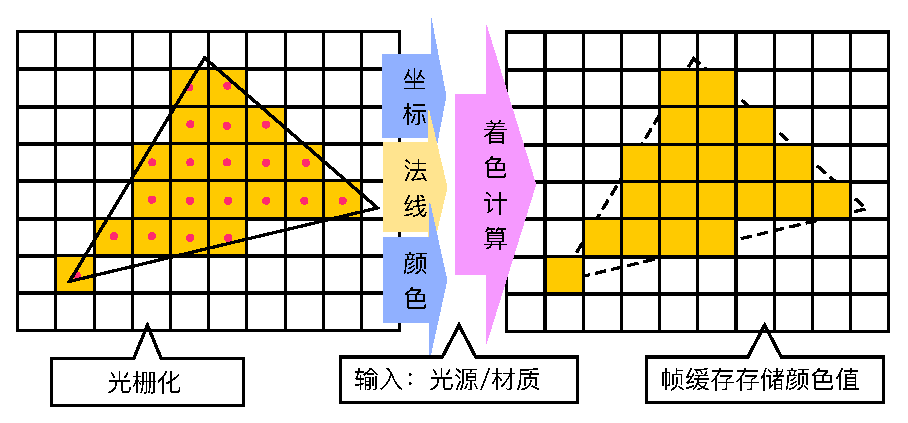
\includegraphics[width=.78\textwidth]{figures/shade/pipeline}
\end{center}
	\caption{利用图形处理器接口提供的渲染管线渲染场景的过程,首先将顶点光栅化为片元,然后根据相关材质参数在片元着色器中计算像素的颜色,帧缓存中的深度缓存被用来剔除被遮挡的片元}
	\label{f:shade-pipeline}
\end{figure}

\begin{enumerate}
	\item 放置一个虚拟摄像机在3D场景中的某个位置,并设置一个视锥体来表示3D世界中的可视区域,这片区域被映射到屏幕上一块2D的具有一定分辨率的窗口。
	\item 场景中每个物体所包含的顶点数据以及绘制该物体所需要的所有环境贴图,阴影等被提交到OpenGL开始绘制该物体,这些顶点所构成的图元被视锥体裁剪\footnote{物体在被绘制之前通常也会在CPU端执行一个基于物体包围盒的3D空间的裁剪。},处于视锥体外部的图元将被丢弃,与视锥体相交的图元将被裁剪,剩下的图元被光栅化到与窗口分辨率对应的像素位置,每个像素块称为一个片元。
	\item 片元着色器对每个片元使用式\ref{eq:shade-shading-equation}进行着色计算,它遍历场景中的每个光源分别计算其对该片元辐射照度的贡献,并将最终结果与帧缓存上对应像素位置上的深度值进行比较,如果通过深度测试则将该颜色值与帧缓存上的颜色值进行混合。
	\item 当所有物体被遍历完后帧缓存上的颜色缓存被送到显示设备进行显示,或者其结果被读回到宿主程序。
\end{enumerate}

这个传统的渲染过程非常简单,它基本上就是直接利用图形处理器接口提供的经典渲染管线,因此它具有所有图形处理器接口提供的便利或优点:

\begin{itemize}
	\item 结合图形接口深度测试和颜色混合的机制,传统的渲染管线可以很容易地实现对半透明物体的绘制。
	\item MSAA被集成到渲染管线,它可以对每个片元的深度进行多次采样,而使用一次着色计算以实现反锯齿。
	\item 每个物体可以根据其图形特征使用独立的着色器或着色器组合。
\end{itemize}

当场景的结构比较简单(拥有较少的物体数量以及光源数量)时,上述的渲染方法非常简单且高效,然而随着场景结构复杂度的增加,该方法会变得非常低效。

在传统的渲染管线中,所有很影响性能的因素几乎都跟一个称为过度绘制(overdraw)\index{过度绘制overdraw}\index[en]{overdraw过度绘制}的概念有关。一般来说,要求得一个摄像机所能看到的场景中的每一个像素点,必须沿从摄像机穿过每一个2D屏幕上像素点的方向上,与整个场景数据做一次相交计算,该方向与场景所有交点的最近点即为屏幕上该点的可视点,然而这样的相交计算非常复杂,所以光栅化技术的核心要点正是简化了这个相交计算:它对整个场景只遍历一次,并记录下屏幕上每个像素点方向上的表面点的深度值,然后让后续的同样落于该像素点的表面点的深度值与该值进行一个简单的深度比较,并保留深度值更小的表面点,这样当整个场景被遍历一遍之后,帧缓存上留下的就是整个场景中所有可视的表面点,这个过程非常高效。然而它的缺陷就是,对于每个表面点,我们必须计算出完整颜色值,即是对其执行式\ref{eq:shade-shading-equation}的计算,这样就导致了过度绘制,因为大量的被遮挡的表面点将被深度测试丢弃,从而导致计算资源的浪费,尤其当场景中有大量光源的时候,式\ref{eq:shade-shading-equation}中需要分别计算每个光源的贡献,这种资源浪费随着光源数量的增加而增加,例如本书后面讲述的即时辐射度方法(参见第\ref{chp:ir}章)可能有上万个虚拟的点光源(VPL),它也随着场景复杂度的增加而增加,因为更多的表面点可能被遮挡。这种渲染性能和场景复杂度的耦合导致的结果是灾难性的,它使得应用程序可能具有极不稳定的帧率。

\begin{figure}
\begin{center}
	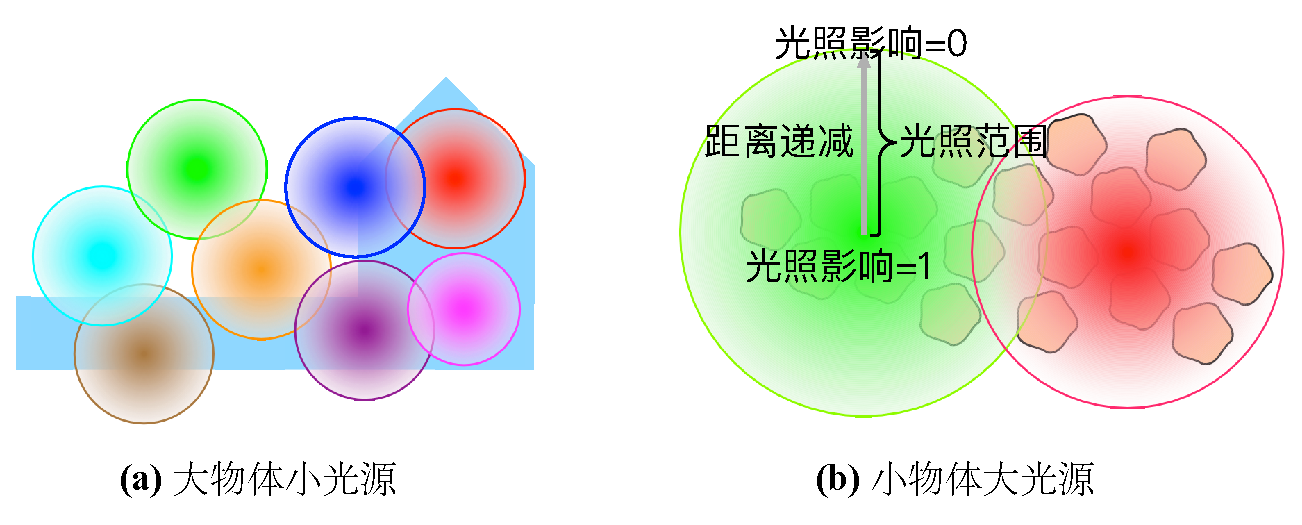
\includegraphics[width=.8\textwidth]{figures/shade/light-culling}
\end{center}
	\caption{当以物体的几何尺寸进行光源剔除时: (a)大物体小光源的场景会使得每个片元可能计算大量无效的光源影响,而(b)小物体大光源的场景会使得大量小物体重复进行光源剔除计算}
	\label{f:shade-light-culling}
\end{figure}

其次,即使是针对有效片元(那些最终没有被深度测试丢弃的片元)的着色计算,由于场景中可能分布成千上万的光源,因此为了提高渲染性能,光源剔除(light culling)\index{光源剔除light culling}\index[en]{light culling光源剔除}十分关键,它要求我们在绘制一个物体之前,应该排除那些对其完全没有影响的光源。这里考虑场景中像直线光源这样对整个场景都有影响的光源还是少数(例如一个场景可能只有一个太阳光源),大部分光源都是点或者其他面积光源,这些光源的辐射强度都受一个距离递减函数\index{距离递减函数distance falloff function}\index[en]{distance falloff function距离递减函数}的影响,如图\ref{f:shade-light-culling}(b)所示,因此光源剔除基本上可以排除大量的无效光源(光照影响为0),从而大大提高渲染性能。光源剔除的目标是使每个片元计算的光源的数量达到最少,有时候我们也称其为光源分配(light assignment)\index{光源分配light assignment}\index[en]{Light assignment光源分配},这是着色管线基础架构的重要内容。

在目前的这种方法中,进行光照剔除的唯一方法是在绘制之前对物体与光源执行包围盒比较,然后只将那些影响该物体的光源信息上传至GPU以进行最节省的片元着色计算。因此为了最大限度降低每个物体受其影响的光源数量,我们应该减少一次绘制的顶点的数量,或者说尽可能每次绘制更少数量的物体,然而这却和每次尽可能绘制更多顶点以降低GPU状态切换的高昂性能代价相矛盾,这个矛盾使得我们很难权衡每次绘制应该选择的批绘制的大小。

当我们以物体的尺寸为依据来选择批绘制块的大小时,如果场景中包含少量大物体和大量小光源时,虽然每个光源可能仅影响大物体的一部分,但是我们不得不对该次绘制使用全部光源,因为以物体的几何尺寸为依据无法剔除这些光源,如图\ref{f:shade-light-culling}(a)所示;同样,当场景中包含大量小物体以及少量大范围的光源时,每个小物体都要单独分别对每个光源进行剔除计算,尽管我们知道多个小物体同时都处于该光源的影响范围之内,如图\ref{f:shade-light-culling}(b)所示。更糟糕的是,场景中可能同时存在这两种情况,因此不管我们怎样权衡,都不可能使每片元计算光源数量达到最低。所以本章后面讲述的着色架构的重要改进就是不以几何物体尺寸,而是以屏幕空间的2D分块(tile)为依据进行光源剔除。

最后,由于传统的渲染管线的着色计算必须在一个片元着色器中完成,因此这些不同的光源组合将导致非常复杂的着色器管理。这些着色器的组合数量是物体类型数量和每种类型不同光源数量(\#lights/type)的一个排列组合。如果我们只使用一个巨大的着色器,在着色器内部使用根据条件进行各种分支切换,这种臃肿包含众多分支的着色器称为大型着色器(uber shader)\index{大型着色器uber shader}\index[en]{uber shader大型着色器},GPU中的大量分支计算将导致非常低的性能,参见第\ref{chp:hardware}章的内容。

同时,也因为所有着色方法被混在一起,所以所有的输入数据不得不随时在内存中处于可用状态,这包括所有的光照图,反射图等等。

由于以上传统渲染管线的各种问题,现代实时渲染方法通常采用改进的方法进行物体表面执行着色计算,这其中最著名的是本章将要讨论的针对过度绘制改进的延迟着色技术,以及在延迟着色技术基础上,针对光源剔除改进的基于2D分块和3D分簇的延迟渲染技术。





\section{延迟着色}
传统的渲染管线使用一个着色器进行整个渲染工作,这个渲染过程其实包括两部分的内容:通过深度测试找出场景中的所有可视点,以及对每个表面点进行着色。利用光栅化技术进行渲染的过程中深度测试是不可避免的(它是图形处理器存在的最重要理由之一),而过度绘制的计算发生于表面着色计算过程,如果我们能够将着色过程和深度测试过程分开,将着色计算延迟到深度测试之后,我们就能避免因被深度测试丢弃片元产生的不必要的着色计算,这就是延迟着色(deferred shading)\index{延迟着色deferred shading}\index[en]{deferred shading延迟着色}技术的原理,与之相对应,我们将传统用于深度测试以确定可视区域的渲染管线称为前向着色\footnote{前向着色的概念其实并不准确,因为第一阶段只是进行深度测试以确定场景中的可视区域,并不涉及表面着色的计算,这里仅仅是为了区分延迟着色中的不同阶段。}(forward shading)\index{前向着色forward shading}\index[en]{forward shading前向着色}。

分析式\ref{eq:shade-shading-equation},要想实现着色计算和深度测试的分离,我们唯一需要做的是对每个深度测试通过的像素使用额外的方式记录下所有这些着色参数,然后使用一个单独的渲染通道来仅对这些可视的像素点进行着色计算。这些包含着色参数的缓存对象称为几何缓存(Geometry buffer,G-buffer)\index{几何缓存geometry buffer,G-buffer}\index[en]{geometry buffer,G-buffer几何缓存},这些着色参数可以使用现代图形处理器接口提供的MRT(参见第\ref{sec:api-framebuffer}节的内容)特性进行存储。

\begin{figure}
\begin{fullwidth}
	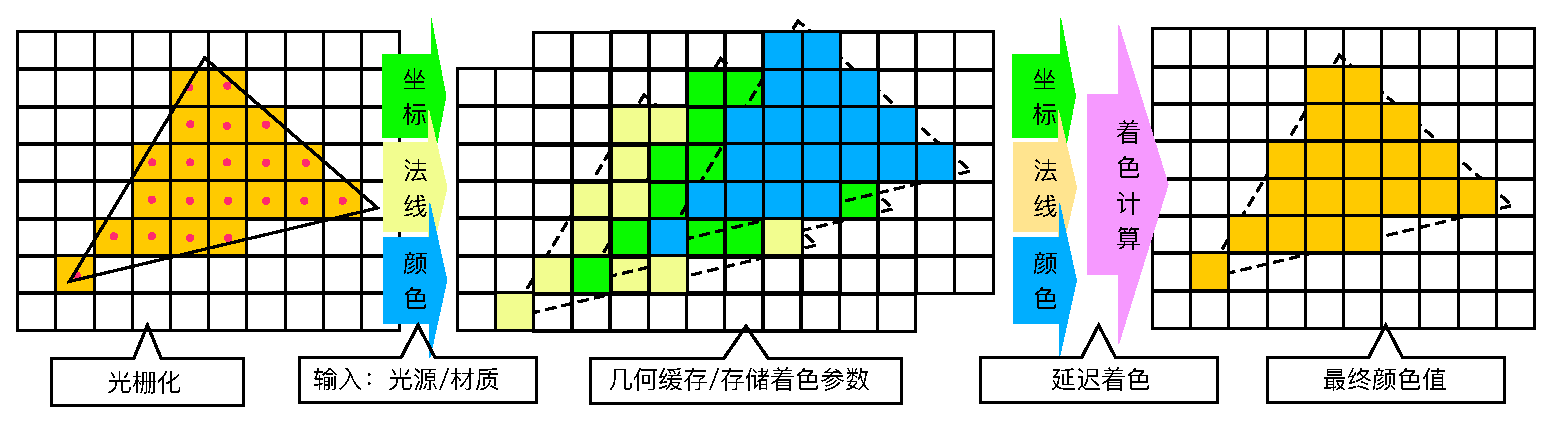
\includegraphics[width=\thewidth]{figures/shade/deferred-pipeline}
	\caption{延迟着色的过程,它在传统的渲染管线基础上,将着色过程和深度测试过程分离,在前向着色阶段仅将着色参数写入到G-buffer中,然后使用一个额外的延迟着色阶段来对像素进行着色计算}
	\label{f:shade-deferred-pipeline}
\end{fullwidth}
\end{figure}

延迟着色的过程如图\ref{f:shade-deferred-pipeline}所示,它可以简述如下:

\begin{enumerate}
	\item 绘制场景中所有的不透明几何体,并将每个片元对应的法线矢量,漫反射折射率,以及高光扩散系数等存储到G-buffer中,如图\ref{f:shade-g-buffer}所示。此过程涉及在片元着色器中输出多个颜色值,因此需要用到图形处理器接口中的MRT特性。此过程称为前向着色\index{前向着色forward shading}\index[en]{forward shading前向着色}阶段。
	\item 分别计算每个光源对可见表面点的影响。这通过分别绘制包围每个光源影响范围的几何体来实现,此时我们应该关闭深度测试,因为我们只需要找出该光源影响的屏幕上的区域,同时每个光源包围几何体有两个面,我们应该根据情况绘制光源包围几何体的其中一面,例如当摄像机位于光源包围几何体内部时,我们应该绘制该几何体的背面,否则只需要绘制正面。对于一些没有体积的光源如直线光源,以及光源影响范围同时包括视锥体近平面和远平面时,我们直接绘制一个2D的包括全屏的平面。在着色器中,前向着色阶段输出的G-buffer将作为纹理数据被读入,G-buffer中的深度值用来计算像素的3D位置,以此用来计算光源的距离递减函数以及查询阴影贴图。最后该光源对每个像素点的颜色计算结果被写入到一个累积缓存(accumulate buffer)\index{累积缓存accumulate buffer}\index[en]{accumulate buffer累积缓存}。此过程称为延迟着色阶段。
	\item 按传统的渲染管线绘制所有半透明的物体。
\end{enumerate}

\begin{figure}
\begin{fullwidth}
	\begin{subfigure}[b]{0.24\thewidth}
		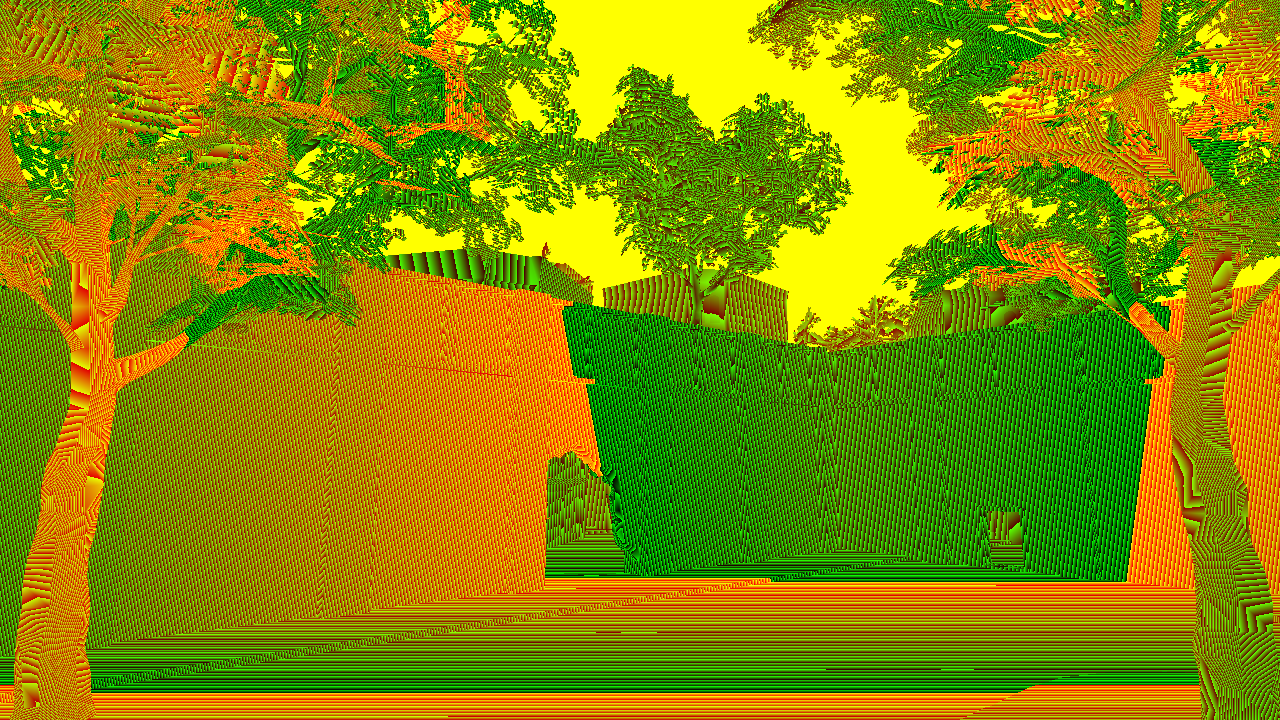
\includegraphics[width=1.\textwidth]{figures/shade/g-buffer-depth}
		\caption{深度+模板}
	\end{subfigure}
	\begin{subfigure}[b]{0.24\thewidth}
		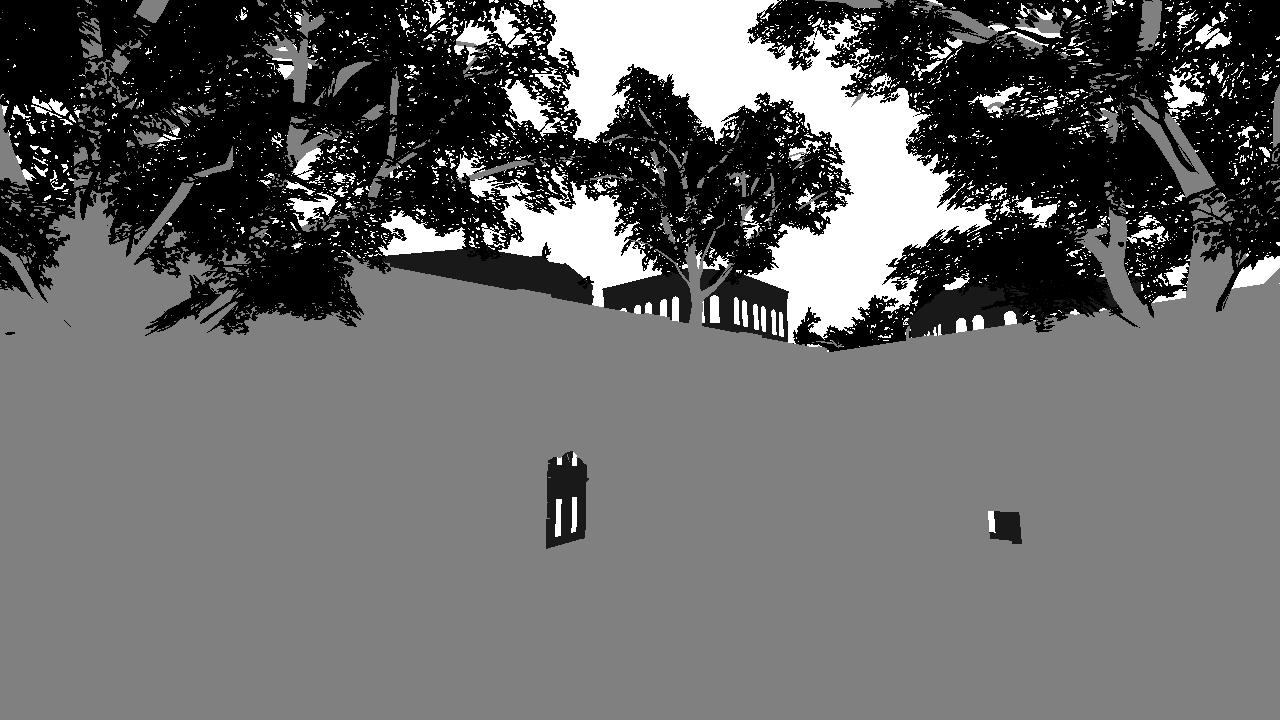
\includegraphics[width=1.\textwidth]{figures/shade/g-buffer-spec}
		\caption{高光扩展系数}
	\end{subfigure}
	\begin{subfigure}[b]{0.24\thewidth}
		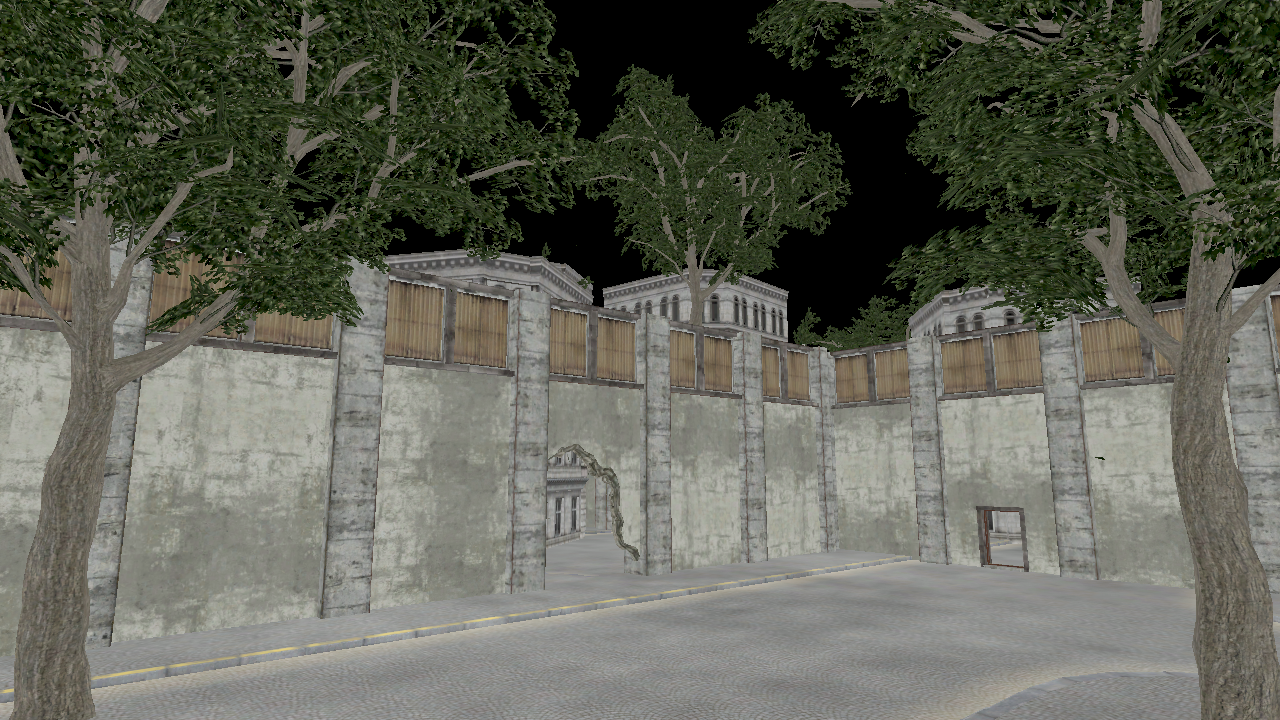
\includegraphics[width=1.\textwidth]{figures/shade/g-buffer-diffuse}
		\caption{漫反射率}
	\end{subfigure}
	\begin{subfigure}[b]{0.24\thewidth}
		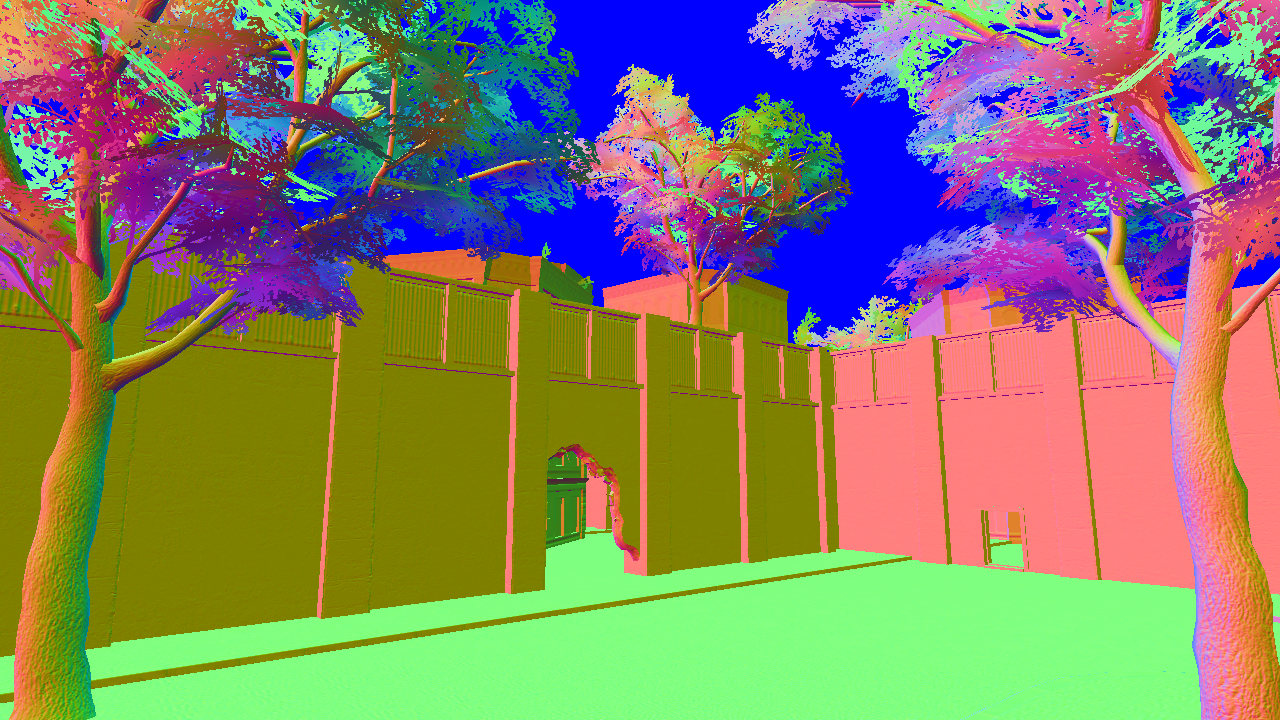
\includegraphics[width=1.\textwidth]{figures/shade/g-buffer-normal}
		\caption{表面法线}
	\end{subfigure}
\caption{一个基本的几何缓存包含深度,漫反射率,表面法线矢量,以及高光扩展系数几个基本的式\ref{eq:shade-shading-equation}中的着色参数,这些着色参数可以被延迟着色(或其他后处理)阶段用于着色计算(图片来自Dice)}
\label{f:shade-g-buffer}
\end{fullwidth}
\end{figure}

延迟着色技术解决了传统渲染管线中的过度绘制的问题,这是通过牺牲内存占用来实现的,它用一个巨大的几何缓存对象将那些着色参数暂存起来,以便能够在稍后待所有不可见的像素被深度测试剔除之后再进行必要的光照计算,能这样做的原因是深度测试本身和着色计算几乎是完全独立的,所以延迟着色计算的结构几乎和传统渲染管线是一致的,并且延迟着色使渲染性能不再与场景的复杂度像耦合(尤其延迟着色支持数量巨大的光源),能够保证稳定的帧率,稳定的帧率是实时渲染领域中的一个重要的衡量指标。

虽然有上述这些优点,并且从渲染结果上看延迟渲染和传统渲染管线的结果是一致的(因为它并没有对式\ref{eq:shade-shading-equation}作任何修改),但是延迟渲染还是带来了一些新的问题,其中一些主要的问题包括:

\begin{itemize}
	\item 不支持半透明物体。一个包含半透明表面的像素点的颜色值是两个(或多个)表面点颜色值混合的结果,由于G-buffer只保存每个像素点的一个表面点的值,所以它不能支持半透明物体,在延迟渲染中我们必须对半透明物体单独采样传统的渲染管线来处理。
	\item 巨大的帧缓存存储占用。通常一个G-buffer中每个像素可以占用多达128bits甚至以上的内存占用,当使用多重采样时更是会占用巨大的内存(我们将在第\ref{sec:shade-anti-aliasing}节讨论延迟着色中多重采样的问题);此外,为了保证多个光源累加结果的精确性,颜色累积缓存还必须使用更高精度的缓存对象。
	\item 对屏幕区域的像素点(而不是根据每个物体自身的类型)进行着色计算,这使得我们很难针对每种物体使用自定义的着色器,因为各种类型的物体被混在一个屏幕区域,我们必须使用统一的着色器,这使得自定义着色器变得非常困难,我们将在第\ref{sec:shade-deferred-custom-shader}节中讨论延迟着色中的着色器管理。
	\item 最后一个问题是内存访问的高带宽占用,这将在本节及接下来的内容中重点介绍。
\end{itemize}

带宽问题是延迟渲染方法带来的新的问题,它带来了一种新的形式的过度绘制,以下是一个传统延迟着色中的着色计算阶段,它对每个光源包围盒形成的几何体绘制一次,然后在其覆盖的屏幕2D区域内对每个像素执行着色计算:

\begin{lstlisting}[language=C++]
for each light
	for each covered pixel
		read G-buffer
		compute shading
		read + write frame buffer
\end{lstlisting}

从以上的伪代码中我们看到,对于每个光源覆盖的每个像素点,着色器都要分别对帧缓存执行:读取-->计算-->写入的操作,如果一个像素点被多个光源所覆盖,这在整个着色计算过程中这个像素点对应的着色数据会被重复读写多次,这就导致一种新的过度绘制。

\begin{figure}
	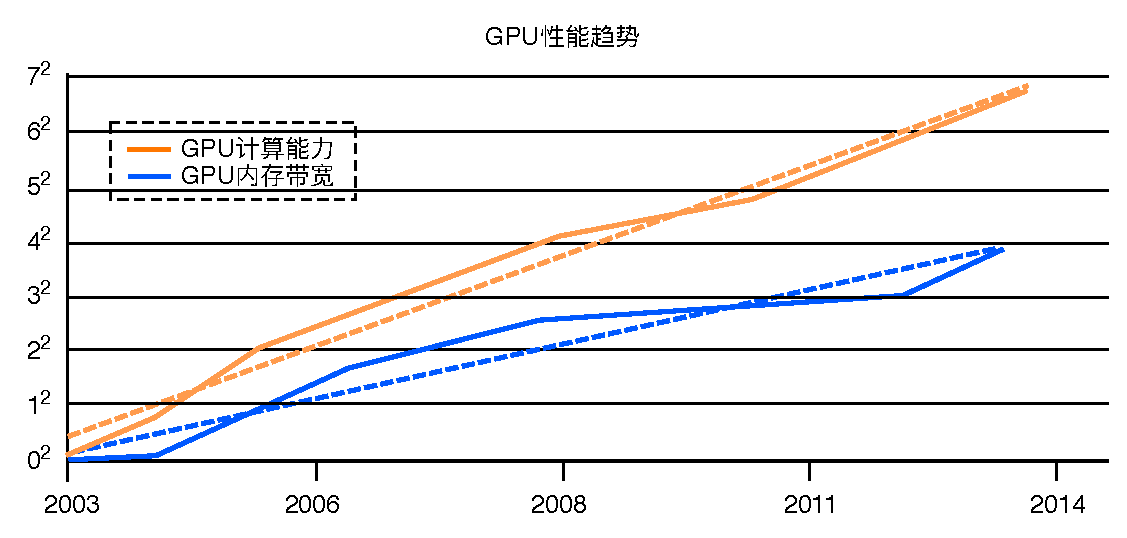
\includegraphics[width=1.\textwidth]{figures/shade/gpu-trends}
	\caption{GPU性能发展趋势,其计算能力的提升速度会大大高于带宽的提升速度,这其实对CPU也是一样的,所以应用程序应该充分优化以更紧密地对数据进行利用,而不是频繁重复地读写}
	\label{f:shade-gpu-trends}
\end{figure}

通过第\ref{chp:hardware}章的内容可知,处理器对任何寄存器以外的内存读取都会导致延迟,这些延迟包括存储器本身处理数据输入输出的延迟,以及数据由存储器向处理器传输过程中带宽的限制。图\ref{f:shade-gpu-trends}是近十几年GPU性能发展的趋势,我们可以看出GPU计算能力提升的速度会大大高于其传输带宽的提升,虽然缓存可以在一定程度上减少带宽导致的延迟,但是它仍然比寄存器要慢得多;同时在GPU中,缓存是基于内核内多个线程共享的,它还必须处理同步的问题。所以在GPU编程中,我们要充分优化内存读写的算法,尽可能低将数据读取到寄存器\footnote{回想第\ref{chp:hardware}章的内容,GPU拥有数量众多的寄存器,将数据读取到本地寄存器,并在单线程内进行足够的计算,然后将最终计算结果写入全局内部是GPU并行计算的基本策略。},对其进行更多计算使用,然后再写入到全局内存中。

针对带宽的问题,我们有两种解决方案:比较好的解决方案是将循环结构中光源的循环放入到双重循环结构的内部,这样针对所有覆盖该表面点的光源只需要对G-buffer中的数据读写一次,但是这需要额外的工作来找出每个表面点被哪些光源覆盖,即所谓的光源分配(light assignment)\index{光源分配light assignment}\index[en]{light assignment光源分配},这种解决方案正是本章后面第\ref{sec:shade-tiled-shading}和\ref{sec:shade-clustered-shading}节的内容,这些方法的重点内容就是解决光源分配。

另一种解决方案,则是减少光源循环中读取数据的数量,即进一步将着色计算中的光照计算分离出来,例如后面的延迟光照方法中,G-buffer中只需要32位存储一个法线矢量即可,大大减少了带宽的占用,本节剩下的内容就将讨论这种减少光源循环中对G-buffer数据读取的数量的方案。





\subsection{延迟光照计算}\label{sec:shade-deferred-lighting}
虽然延迟着色将着色计算与深度测试分离开来,使得着色计算仅针对屏幕空间中的像素点进行,从而大大节省计算资源,但我们仍然面临光源循环导致的帧缓存数据重复读取的计算资源浪费,于是我们想要进一步从着色计算中抽离出仅与光源相关的部分,这样就可以节省出光源循环中对帧缓存数据的重复读取。

渲染方程通常拆分成漫反射和高光反射,所以式\ref{eq:shade-shading-equation}可以写成如下的形式:

\begin{equation}
	L_o(\mathbf{v})=\sum^{n}_{k=1}\bigg(\mathbf{c}_{\rm diff}\otimes f_{\rm diff}(E_{L_k},\mathbf{l}_k,\mathbf{n})+\mathbf{c}_{\rm spec}\otimes f_{\rm spec}(E_{L_k},\mathbf{l}_k,\mathbf{n},\mathbf{v},m)\bigg)
\end{equation}

\noindent 考虑到物体表面的反射率是由材质提供的常数,所以上式可以进一步写成:

\begin{equation}\label{eq:shade-deferred-lighting}
	L_o(\mathbf{v})=\mathbf{c}_{\rm diff}\otimes\sum^{n}_{k=1}f_{\rm diff}(E_{L_k},\mathbf{l}_k,\mathbf{n})+\mathbf{c}_{\rm spec}\otimes \sum^{n}_{k=1}f_{\rm spec}(E_{L_k},\mathbf{l}_k,\mathbf{n},\mathbf{v},m)
\end{equation}

分析上式,我们可以将漫反射率和高光反射率从着色方程中抽离出来,使得与光源相关的计算部分只剩下法线和高光扩展系数,而光源入射方向是可以从法线方向计算出来的。因此,按照这样的拆分,我们可以只需要在G-buffer中存储法线和高光扩展系数,法线是一个RGB颜色值,高光扩散系数通常是一个很小的整数,因此整个G-buffer只需要一个32位的颜色缓存(即是光照计算的延迟着色器中只需要读写一个32位而不是128位甚至更多的数据)即可,这种情况下甚至不需要硬件支持多目标渲染(MRT)。

不过此时我们需要两个累积缓存来分别保存漫反射和高光反射部分“辐射照度”的值,它们分别是:

\begin{equation}
\begin{aligned}
	g_{\rm diff}&=\sum^{n}_{k=1}f_{\rm diff}(E_{L_k},\mathbf{l}_k,\mathbf{n})\\
	g_{\rm spec}&=\sum^{n}_{k=1}f_{\rm spec}(E_{L_k},\mathbf{l}_k,\mathbf{n},\mathbf{v},m)
\end{aligned}
\end{equation}

当光照计算阶段完成之后,我们再对场景使用渲染管线执行第二次渲染,但是此时的着色计算仅需要从上述两个累积存储中取出辐射照度的数据,然后依照下式进行计算即是最终的着色颜色值:

\begin{equation}
	L_o{\mathbf{v}}=\mathbf{c}_{\rm diff}\otimes g_{\rm diff}+\mathbf{c}_{\rm spec}\otimes g_{\rm spec}
\end{equation}

如果硬件支持MRT,我们同样可以直接将法线以外的材质数据保存在G-buffer中,所以第二次几何通道不需要重新渲染整个场景,而仅对屏幕空间执行一次渲染即可。延迟光照计算的渲染过程如图\ref{f:shade-deferred-lighting}所示。

\begin{figure}
\begin{fullwidth}
	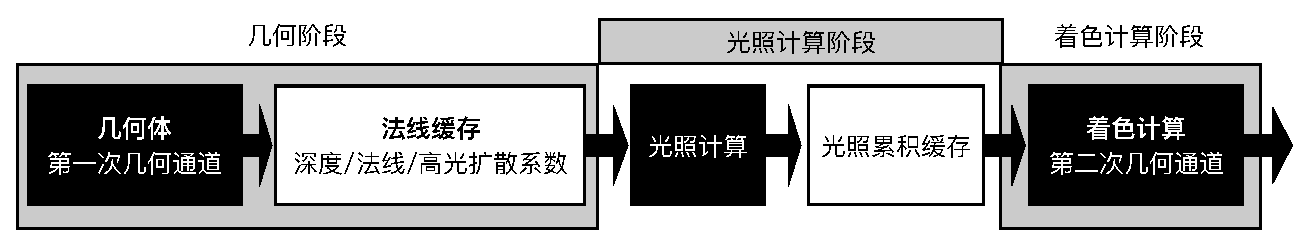
\includegraphics[width=\thewidth]{figures/shade/deferred-lighting}
	\caption{延迟光照计算中的各个阶段,首先光照计算需要的表面属性被写入到一个法线缓存中,然后光照计算读取法线缓存中的数据将计算出的辐射“辐射照度”信息写入到光照累积缓存中,最后在对场景执行一次光栅化,并直接读取光照累积缓存中的数据对像素点进行最终着色计算}
	\label{f:shade-deferred-lighting}
\end{fullwidth}
\end{figure}

由上述内容可知,延迟光照计算的过程可以简述如下:

\begin{enumerate}
	\item 渲染场景中所有不透明的几何体,并将法线矢量$\mathbf{n}$和高光扩展系数$m$写入到帧缓存中,由于法线矢量占据三个分量,而高光扩展系数是一个很小的整数,所以它们可以被合进一个“n/m缓存”,这只需要一个4分量的颜色缓存即可,所以可以不需要MRT的支持。此过程称为第一个几何通道。
	\item 和延迟着色一样,该阶段逐个渲染每个光源包围盒所在的几何体,并对该光源覆盖的每个屏幕像素点进行光照计算;和延迟着色不一样的是,它只计算“辐射照度”而不是辐射亮度,并且最终输出的漫反射和高光反射的辐射照度被写入到两个累积缓存中。此阶段为延迟光照计算阶段。
	\item 重新渲染所有不透明几何体,但是此时并不需要对表面进行光照计算,它仅仅需要从前一阶段的两个颜色累积缓存中读取值执行式\ref{eq:shade-deferred-lighting}的计算即可。并将最终的着色结果写入到帧缓存中。此阶段为第二次几何通道。
	\item 绘制所有半透明的物体。
\end{enumerate}

延迟光照计算方法被大量使用于游戏引擎中,其中对其进行优化的地方主要集中于延迟光照计算阶段输出的两个辐射照度量的存储表述。每个颜色值分别包含RGB三个通道,所以需要两个各自具有3通道的颜色缓存对象来存储,在Crytek的CryEngine3\cite{a:AbitmoreDeferred-CryEngine3}引擎中,他们使用一个4通道的颜色缓存(A16R16G16B16f或A8R8G8B8)来同时记录漫反射和高光反射的辐射照度,其中前3个通道表示漫反射值diffuse,第4个通道表示高光的强度strength,所以高光的颜色值可以由diffuse*strength计算得出,它的效果如图\ref{f:shade-deferred-lighting-crytek}所示。

\begin{figure}
	\begin{subfigure}[b]{0.49\textwidth}
		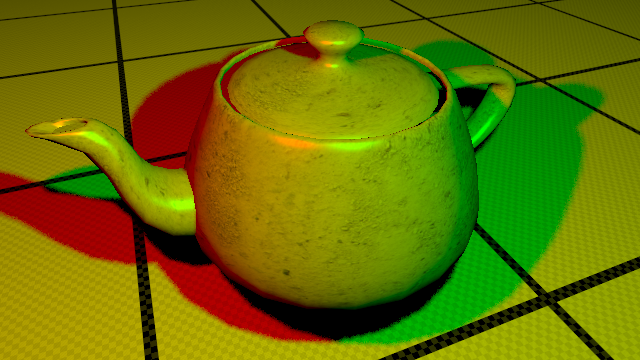
\includegraphics[width=1.\textwidth]{figures/shade/tea0}
		\caption{原始6通道}
	\end{subfigure}
	\begin{subfigure}[b]{0.49\textwidth}
		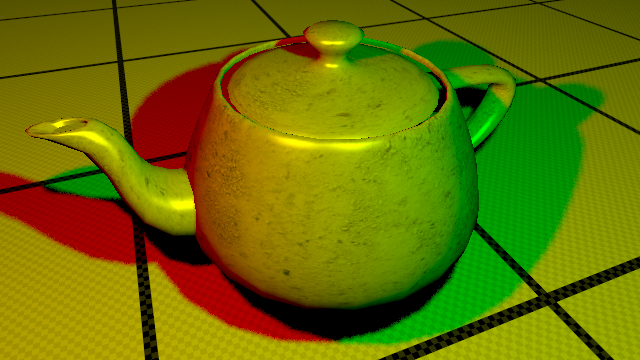
\includegraphics[width=1.\textwidth]{figures/shade/tea1}
		\caption{4通道}
	\end{subfigure}
\caption{Crytek在CryEngine3中使用一个4通道的颜色缓存来同时记录漫反射和高光反射(图片来自Crytek)}
\label{f:shade-deferred-lighting-crytek}
\end{figure}

Crytek并没有说明他们使用何种方法来编码高光反射的值,但是从图\ref{f:shade-deferred-lighting-crytek}可以看出,其中茶壶同时被一个红色光源和一个绿色光源照亮,图\ref{f:shade-deferred-lighting-crytek}(a)的原始6通道的颜色缓存能够准确反应反射物体的颜色,它的边沿上呈现红绿两种高光,而4通道的方案失去了反射环境的颜色,所以它仅仅保留了高光的亮度(luminance)\index{亮度luminance}\index[en]{luminance亮度},而丢弃了高光的色度(chrominance)\index{色度chrominance}\index[en]{chrominance色度}。因为人眼对于高光的亮度感应较色度更为明显,所以一般情况下没有太大问题。Pavlos Mavridis等\cite{a:TheCompactYCoCgFrameBuffer}提出了一种帧缓存的压缩方法可以用一个4分量的颜色缓存更精确地存储两个颜色值,它的效果如\ref{f:shade-deferred-lighting-1}(c)图所示。

\begin{figure}
	\begin{subfigure}[b]{0.32\textwidth}
		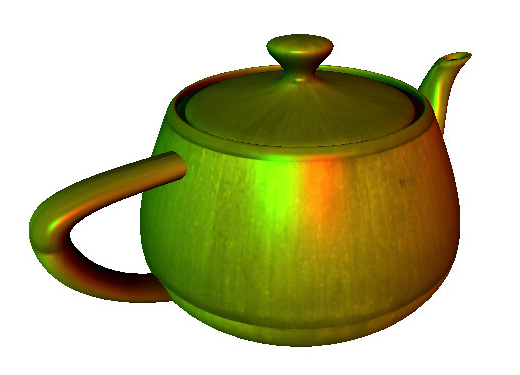
\includegraphics[width=1.\textwidth]{figures/shade/deferred-lighting-1}
		\caption{原始6通道}
	\end{subfigure}
	\begin{subfigure}[b]{0.32\textwidth}
		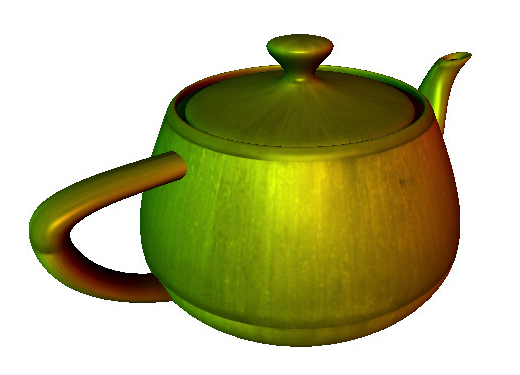
\includegraphics[width=1.\textwidth]{figures/shade/deferred-lighting-2}
		\caption{4通道}
	\end{subfigure}
	\begin{subfigure}[b]{0.32\textwidth}
		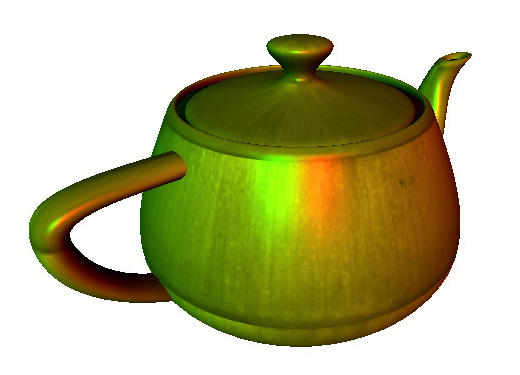
\includegraphics[width=1.\textwidth]{figures/shade/deferred-lighting-3}
		\caption{压缩帧缓存}
	\end{subfigure}
\caption{使用YCoCg压缩帧缓存用一个4通道的颜色缓存可以准确存储高光的色度和亮度,(b)中的方案直接丢弃色度而仅保留亮度,所以在高光部分看不出光源的颜色}
\label{f:shade-deferred-lighting-1}
\end{figure}









\section{光源分配}\label{sec:shade-light-assignment}
针对延迟着色方法的高带宽占用,我们在上一节中介绍了第一种方法,即通过减少光源循环内每个像素读写G-buffer中缓存数据量的大小来减少带宽的占用,这主要是通过式\ref{eq:shade-deferred-lighting}来实现。

降低带宽占用的另(也是最重要的)一个方法是改变传统延迟着色中的循环结构,使像素的遍历处于外循环,而光源的遍历处于内循环,这样将使得G-buffer中的材质参数只被读写一次,调整后的伪代码如下所示:

\begin{lstlisting}[language=C++]
for each pixel 
	read G-buffer
	for each affecting light
		compute shading
	write frame buffer
\end{lstlisting}

然而这样的循环结构调整带来了渲染流程的巨大变化,首先,我们不能再以一个个光源的包围盒几何体为绘制单元进行绘制,而只能使用一个覆盖全屏区域的四边形进行绘制,这意味着所有光源类型都必须使用同一个着色器,特殊光源不能再使用独立的着色器,所以着色器的管理变得更加复杂,这部分的内容参见第\ref{sec:shade-deferred-custom-shader}节。

其次,在处理每个像素的时候,必须知道每个像素受哪些光源影响。我们不能使用一个全局的包含全部光源的一个列表,因为这个列表可能包含上千个光源,这将会导致巨大的计算资源的浪费。考虑到通常场景中的局部区域只受少量的光源的照射\footnote{有些游戏引擎还会限制每个物体或者某些区域受影响的最大光源数量。},所以针对每个像素点的光源分配(light assignment)\index{光源分配light assignment}\index[en]{light assignment光源分配}变得非常重要\footnote{光源分配可以说是实时渲染非常重要的一个话题,现代很多具有复杂场景的游戏往往都有大量的各种类型的光源,即使场景中没有那么多真实的光源,有些渲染技术也可能包含大量虚拟的光源(例如本书后面将会讲述的即时辐射度方法就可能包含上千个虚拟点光源),因此光源分配几乎是现代游戏引擎必然会涉及的内容。},接下来我们将会讨论两种重要的光源分配方案。






\subsection{分块着色}\label{sec:shade-tiled-shading}
使用全局的光源列表是非常低效的,我们也不可能针对每个可视的表面点都执行光源分配计算,那样光源分配计算本身的开支都是很大的,并且光源分配的结果需要更大的缓存对象来存储。相反,我们找到一种折中的方法,即让一个区域内相邻的表面点共享一个光源列表,这样做的原因是相邻的表面点一般拥有相同的光源列表。

分块着色(tiled shading)\index{分块着色tiled shading}\index[en]{tiled shading分块着色}将屏幕区分划分为由多个块(tile)组成的网格(grid),每个块覆盖的像素区域\footnote{当然也可以根据性能分析选择其他尺寸的块,本书以$32\times 32$块大小为例讨论。}为$32\times 32$,每个块拥有一个独立的光源列表,它表示该区域内所有像素点受影响的光源列表,块内的所有像素点共享整个光源列表,如图\ref{f:shade-tiled-shading}所示。

\begin{figure}
\begin{center}
	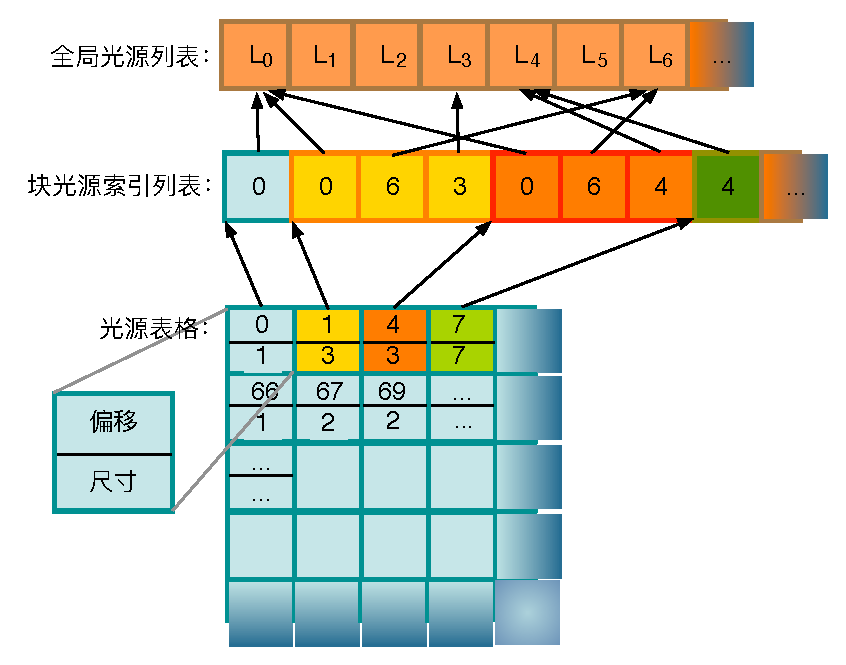
\includegraphics[width=0.75\textwidth]{figures/shade/tile-grid}
\end{center}
	\caption{分块着色块光源列表的数据结构,全局光源列表存储着所有光源的ID,块光源索引列表连续地存储这每个块对应的所有光源的索引值,这样每个块通过一个偏移值和尺寸即可从块光源索引列表中取出该块的光源ID列表}
	\label{f:shade-tiled-grid}
\end{figure}

全屏块表格的数据结构如图\ref{f:shade-tiled-grid}所示,所有块存储为一个2D纹理,如图\ref{f:shade-tiled-grid}下面的正方形表格,每个像素点可以通过在屏幕区域的像素位置来计算其块索引,每个块存储两个数据:偏移和尺寸,所有块的光源列表存储在一个大的全局光源索引列表中,该索引列表中的每个值指向全局光源列表的一个光源,每个块通过在全局光源索引列表中的偏移值和尺寸来选择该块对应的光源列表。

对于块表格结构数据的填充,最简单的方法是将每个光源的包围盒矩形投射到屏幕上,然后在每个块中分别插入受其影响的光源索引到全局光源索引列表中,并修改块数据中的偏移和索引值,如图\ref{f:shade-tiled-shading}所示,该场景包含两个光源,重叠部分的块的光源列表将包含两个光源,未被光源包围盒投射的块则不包含任何光源\footnote{注意这些块虽然没有任何直接的光源照射,它仍然可能被环境光,天空盒等其他形式的光源照射。},其他受单个光源影响的区域包含一个光源。

\begin{figure}
	\includegraphics[width=1.0\textwidth]{figures/shade/tiled-shading}
	\caption{使用将光源包围盒直接投射到屏幕区域来建立块光源列表的数据,这里的数字仅用于演示表示光源的数量,它的真实数据结构如图\ref{f:shade-tiled-grid}所示}
	\label{f:shade-tiled-shading}
\end{figure}

这种方法虽然简单,但是它在一些块中插入了无效的光源,例如在一个点光源的四个角的位置,或者表面点在垂直于屏幕方向上距离光源位置很远,从而其根本不会受到该光源影响,但是它同样处于该光源投射的区域。一些方法使用模板测试,类似阴影体积(shadow volume)\myindex{阴影体积}{shadow volume}的方法来精确地关联光源与其影响的块,另一些方法给表面点设定一个最近和最远受光源影响的距离,来排除一些距离比较远的光源的影响。我们将在下一节分簇着色中讨论一个更详细的示例。

块数据的建立可以发生在GPU中,也可以在CPU中处理,例如Dice在Battlefield 3\cite{a:SPU-basedDeferredShadingforBattlefield3onPlaystation3}中就是将分块的数据从GPU读回到CPU,然后在SPU中处理块的数据。不但如此,他们还在SPU中执行块的着色计算,每次处理一个完整块内的所有像素,这样还可以减少一个块内光源列表的重复读取。


光源分配的结果既可以适用于传统的前向分块着色\cite{a:ForwardBringingDeferredLightingtotheNextLevel}(tiled forward shading)\index{前向分块着色tiled forward shading},也可以适用于延迟分块着色(tiled deferred shading)\index{延迟分块着色tiled deferred shading}\index[en]{tiled deferred shading延迟分块着色}中。然而不管使用什么样的着色管线,光源分配几乎都具有以下的三个阶段:

\begin{enumerate}
	\item 对场景(不透明的物体)执行一次无光照的传统的渲染管线,以确定哪些像素是可见的,这通常就是延迟着色的前向着色阶段。
	\item 利用某种方法对上述可视的表面点执行光源分配(例如基于分块的方案或基于分簇的方案,见本节后面的内容),它输出一个针对每个可视表面点的光源列表。
	\item 利用光源列表执行每个可视表面点的光照计算。
\end{enumerate}

因为我们不可能对场景中所有像素或区域都执行光源分配,所以无论使用前向或者延迟着色方法,都必须要有一个前向的深度测试阶段来避免不必要的光源分配计算。因此如果你使用的是前向着色方法(例如\cite{a:ForwardBringingDeferredLightingtotheNextLevel}中的Forward+),则至少需要包含两个前向渲染阶段,这时第一个阶段往往称为pre-z pass。

对于延迟分块着色,它仅仅是增加了一个光源剔除的阶段,所有它拥有和延迟着色几乎一样的优点和缺点。针对光源剔除来讲,分块着色还存在很大的优化空间,由于分块着色将3D空间投射到2D的屏幕区域,因此它的每个块占据了深度方向上非常大的范围,如图\ref{f:shade-tiled-problem}所示,在分块1中,两个物体之间存在深度不连续(depth discontinuities)\index{深度不连续depth discontinuities}\index[en]{depth discontinuities深度不连续},我们无法用简单的分块范围(一个最大最小深度范围值)来剔除包含在中间的光源,所以这导致无效的光源被计算在分块光源列表中;例如对于分块3,它的深度是连续的,但是同样由于深度范围太多,使得该分块必须包含该深度范围内的所有光源。

\begin{figure}
	\sidecaption
	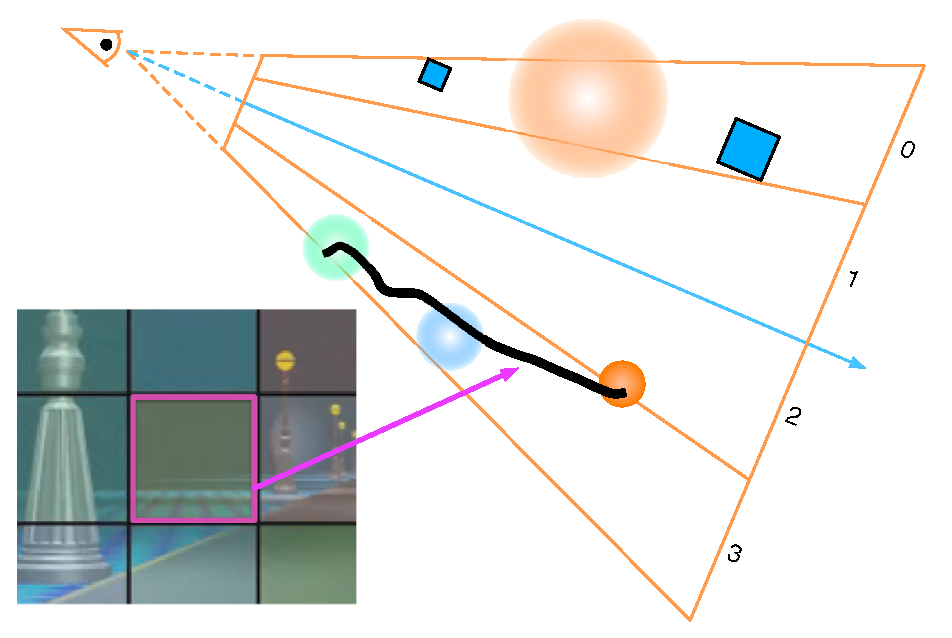
\includegraphics[width=0.65\textwidth]{figures/shade/tiled-problem}
	\caption{分块着色仅仅将3D空间投射到一个2D的屏幕区域,所有每个分块包含了过度的光源信息,影响了着色计算时的计算性能,数字1,2,3,4表示分块索引,分块4对应的小图表示一段深度连续的路面,这种情况在游戏中很常见}
	\label{f:shade-tiled-problem}
\end{figure}

使用2D分块的另一个问题是这些分块信息是与视点相关的(view dependent)\index{视点相关的view dependent}\index[en]{view dependent视点相关的},即一旦摄像机位置和方向发生移动,或者场景中的某些物体位置发生改变\footnote{也包括光源位置改变,但此处仅改变光源颜色不影响光源分配。},则整个分块表格的数据需要重新计算。分块着色的这些问题使得我们将目光转向了3D的分簇着色。





\subsection{分簇着色}\label{sec:shade-clustered-shading}
为了进一步剔除光照计算阶段每个像素点受影响的光源数量,分簇着色\cite{a:ClusteredDeferredandForwardShading}(clustered shading)\index{分簇着色clustered shading}\index[en]{clustered shading分簇着色}在分块着色的基础上将像素分组的划分从2D的屏幕空间(screen space)\index{屏幕空间screen space}\index[en]{screen space屏幕空间}延伸到3D的观察空间(view space)\index{观察空间view space}\index[en]{view space观察空间},与之相应,每个3D的块称为一个簇(cluster)\index{簇cluster}\index[en]{cluster簇},从而使每个光源真正做到仅影响其局部区域。

分簇着色的基本步骤如下:

\begin{enumerate}
	\item 将几何场景渲染到G-buffer以获取有效可视表面点及其相关材质属性。
	\item 计算每个簇的索引键值(cluster key)\index{索引键值cluster key}\index[en]{cluster key索引键值},也称为簇分配。
	\item 找出唯一的簇集合。
	\item 分配光源到每个簇。
	\item 利用每个簇的光源列表对像素点进行着色计算。
\end{enumerate}

其中第一步和传统的延迟着色或分块着色并没有什么区别;第二步对每个像素点执行一次计算,它根据像素点的位置(也可以加入法线的限制)计算出每个像素点的的簇索引键值;然后第三步将这些簇索引键值合并,以形成一个包含唯一键值的簇列表;第四步则将光源分配到每个簇;最后第五步根据每个像素所在簇的光源列表对像素点进行着色。





\subsubsection{簇分配}
对3D空间执行某种空间结构的划分,都可能导致大量的空域,比如场景中会有大量空间位置不包含最终屏幕上呈现的像素点。传统的几何空间的划分可以使用如BVH这样的树状结构来忽略大部分空域,但是分簇着色使用的是一种特殊的子空间结构(见下面的内容),并不能用简单地用树状结构进行管理。所以分簇着色使用一种特殊的方式来构建簇集合:它对每个可视像素点都做一个簇索引键值的计算,这样遍历完所有像素点后的簇索引键值就是有效的簇,然后去掉重复的(即一个簇内的像素点计算出相同的索引值)簇索引键值,就形成一个有效的簇列表。

簇分配的第一个问题涉及怎样表述每一个簇的空间结构,因为这关系到簇索引键值怎样计算,一般的按一个固定尺寸的正方体(uniform grid)的划分会导致离摄像机较远的区域拥有非常密集的簇,所以其簇的密度几乎接近于像素的大小,这显然增加了后面光源分配的计算量;考虑到我们仅仅对视锥体内的点感兴趣,即观察空间(view space)\index{观察空间view space}\index[en]{view space观察空间},所以分簇着色技术对视锥体进行划分,它以分块着色中2D屏幕上块的划分为基础,然后在深度方向上添加一个细分维度,如图\ref{f:shade-clusters}所示,这样划分的每个子空间称为一个簇(cluster)\index{簇cluster}\index[en]{cluster簇},或者子视椎体(sub frustum)\index{子视椎体sub frustum}\index[en]{sub frustum子视椎体},或者视锥体素(frustum voxel,froxel\footnote{这是一个来自\cite{a:Learningfromfailure}中的概念。})\index{视锥体素frustum voxel,froxel}\index[en]{frustum voxel,froxel视锥体素}。

\begin{figure}
\begin{fullwidth}
	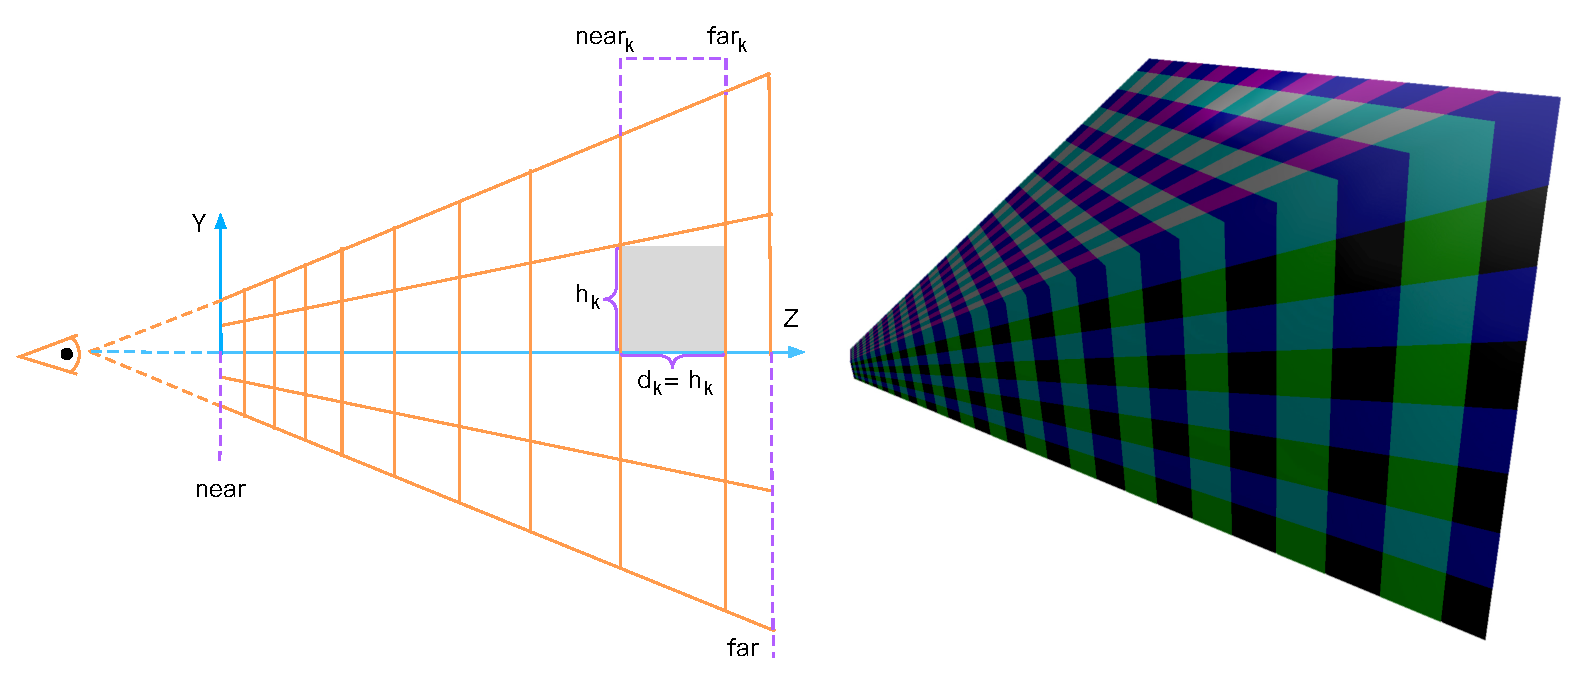
\includegraphics[width=\thewidth]{figures/shade/clusters}
	\caption{分簇着色使用的是一种针对视锥体空间进行划分的方法,它以分块着色的块在基础,在深度方向上按指数形式进行划分,每个子空间称为一个簇,左图仅列出屏幕空间Y方向}
	\label{f:shade-clusters}
\end{fullwidth}
\end{figure}

由于经过摄像机的透视投影,同样大小的物体在更远的在屏幕上所占的空间更小,所以分簇着色没有在深度方向上使用平均长度划分,而是以指数的形式划分深度方向,即更远的地方簇的尺寸更大,更近的地方簇的尺寸更小,如图\ref{f:shade-clusters}所示,这样每个簇的尺寸更接近于一个立方体。

那么,怎样通过一个屏幕坐标系的像素点位置计算出该像素点所在的簇的索引键值呢?假设在屏幕空间Y方向细分子空间(在屏幕空间每个块的大小为$32\times 32$像素)的数量为$S_y$,则深度方向上第$k$个子视锥体\footnote{注意这里指的是包含第$k$层上所有的簇子椎体,如图\ref{f:shade-clusters}左边顶部的虚线所指示的部分。}的近平面$near_k$在Y方向的长度为:

\begin{equation}
	near_k=near_{k-1}+h_{k_1}
\end{equation}

\noindent 对于第一个子视锥体,$near_0=near$($near$表示整个摄像机视锥体的近平面Y方向上的长度),对于一个$2\theta$的张角,有以下关系:

\begin{equation}
	h_0=\frac{2near\tan{\theta}}{S_y}
\end{equation}

\noindent 其中,$h_k$表示第$k$级子视锥体上每个簇在Y方向的长度,由此可以得出:

\begin{equation}
	near_k=near(1+\frac{2\tan{\theta}}{S_y})^k
\end{equation}

\noindent 由于每个簇在深度方向上的长度:$d_k=h_k$,如图\ref{f:shade-clusters}所示,则解出$k$的值为:

\begin{equation}
	k=\Bigg\lfloor \frac{\log{(-z_{vs}/near)}}{\log{(1+\frac{2\tan{\theta}}{S_y})}} \Bigg\rfloor
\end{equation}

\noindent 这里${\rm floor}(x)=\lfloor x\rfloor$称为一个下取整函数(floor function)\index{下取整函数floor function}\index[en]{floor function下取整函数},它表示取小于或等于$x$的最大整数,对于的上取整函数(ceiling function)\index{上取整函数ceiling function}\index[en]{ceiling function上取整函数}为${\rm ceiling}(x)\lceil x\rceil$表示取大于或等于$x$的最小整数。

利用上式我们便可以计算出一个用三元组$(i,j,k)$表示的簇索引键值,假设$(x_{ss},y_{ss})$表示像素点在屏幕空间(screen space)的坐标,$(t_x,t_y)$分别表示屏幕空间每个块的尺寸,则$(i,j)=(\lfloor x_{ss}/tx\rfloor,\lfloor y_{ss}/t_y\rfloor)$;$z_{vs}$表示观察空间(view space)的深度值。

所以,给定一个像素点的坐标,我们便可以计算出该像素点所在簇的索引键值,这个索引键值由$(i,j,k)$三元组表示。在\cite{a:ClusteredDeferredandForwardShading}的实现中,他们为$i,j$分量分别分配8位,而$k$分量分配10位,所以总共需要26位的长度来表示一个簇索引键值。

分簇着色中簇的索引值键值并没限定只能使用空间坐标来表示,它还可以使用更高的维度来使光源分配的数量更接近实际有效的光源数量。在\cite{a:ClusteredDeferredandForwardShading}中还可以为一个簇指定该簇内像素点的法线分布,从而可以有效地进行背面剔除(back-face culling)。为此,它们为索引键值增加了6位用来表示法线分布,这样簇的索引键值就变成32位,可以使用一个32位的颜色值表示,其中包含$(i,j,k,normal)$四个分量。

为了使用有限的数据长度表示法线的空间分布,他们使用一个假想的立方体来表示空间分布,6位数据长度可以用来表示64个位的组合,所以立方体可以被细分为$3\times 3$个的子立方体,每个面的每个立方体分别表示一个锥型(cone)\index{锥型cone}\index[en]{cone锥型}\footnote{为了计算简便,这里不会表述严格的法线空间分布,而仅仅是用每个子立方体代表一个锥形范围,如果包含多个子立方体方向,则将它们合并为更大范围的锥形,这样实际是夸大了法线分布的范围,但是这对于光源密集的区域,存在背面剔除的光源的数量还是很大的,大部分表面的法线分布都在一个很小的范围内。}的空间范围,这样一共需要$3\times 3\times 6=54$个位组合,如图\ref{f:shade-normal-cone}左边所示。

\begin{figure}
\sidecaption
	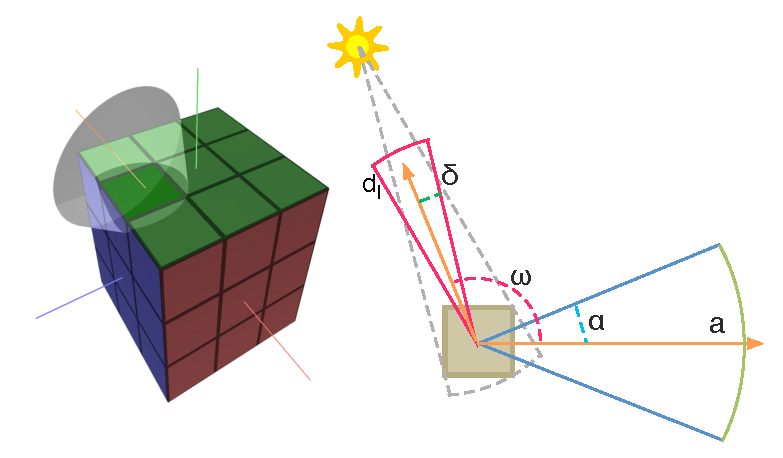
\includegraphics[width=.65\textwidth]{figures/shade/normal-cone}
	\caption{每个簇内像素的法线分布用一个$3\times 3$的立方体表示,立方体每个面的每个细分面表示一个锥形的法线分布范围,54个位的组合可以由每个像素点分别计算出来}
	\label{f:shade-normal-cone}
\end{figure}

当法线分别被提供之后,表面背面的光源可以进一步被剔除\footnote{利用法线分布来剔除背面的光源,在Battlefield 3中又称为法线剔除(normal culling)\index{法线剔除normal culling}\index[en]{normal culling法线剔除}。}。如果入射光方向(从光源到簇中心位置的方向)与法线锥形的中心轴之间的夹角$\omega$大于$\pi /2+\alpha+\delta$,则该光源应该被剔除。这里$\alpha$是法线锥形的半角(half angle),$\delta$是从光源发出的包围簇的AABB包围盒的锥形的半角,如图\ref{f:shade-normal-cone}右边所示。






\subsubsection{找出唯一的簇集合}
当每个像素点所在的簇索引键值被计算出来以后,形成一个包含重复键值的簇索引键值列表,这时我们需要压缩该列表,去除重复的部分(同一个簇内的所有像素点拥有相同的簇索引键值),以形成一个包含唯一簇索引键值的簇列表,如图\ref{f:shade-sorted-key}所示。

由于2D屏幕空间相邻像素点所在的簇在3D观察空间上并不一定是连续的\footnote{例如由于表面不连续导致两个像素点在深度方向上的距离很远,此时虽然它们在2D的屏幕空间相邻,但是所在的簇并不相邻。},所以这些由像素点计算出的簇索引键值也并不一定是连续的,如图\ref{f:shade-sorted-key}上图。因此要想去除重复键值,最简单的方法就是首先对索引键值列表进行排序,如图\ref{f:shade-sorted-key}中间小图,然后去除掉每一段重复的索引键值即可,如图\ref{f:shade-sorted-key}下图。

\begin{figure}
\begin{center}
	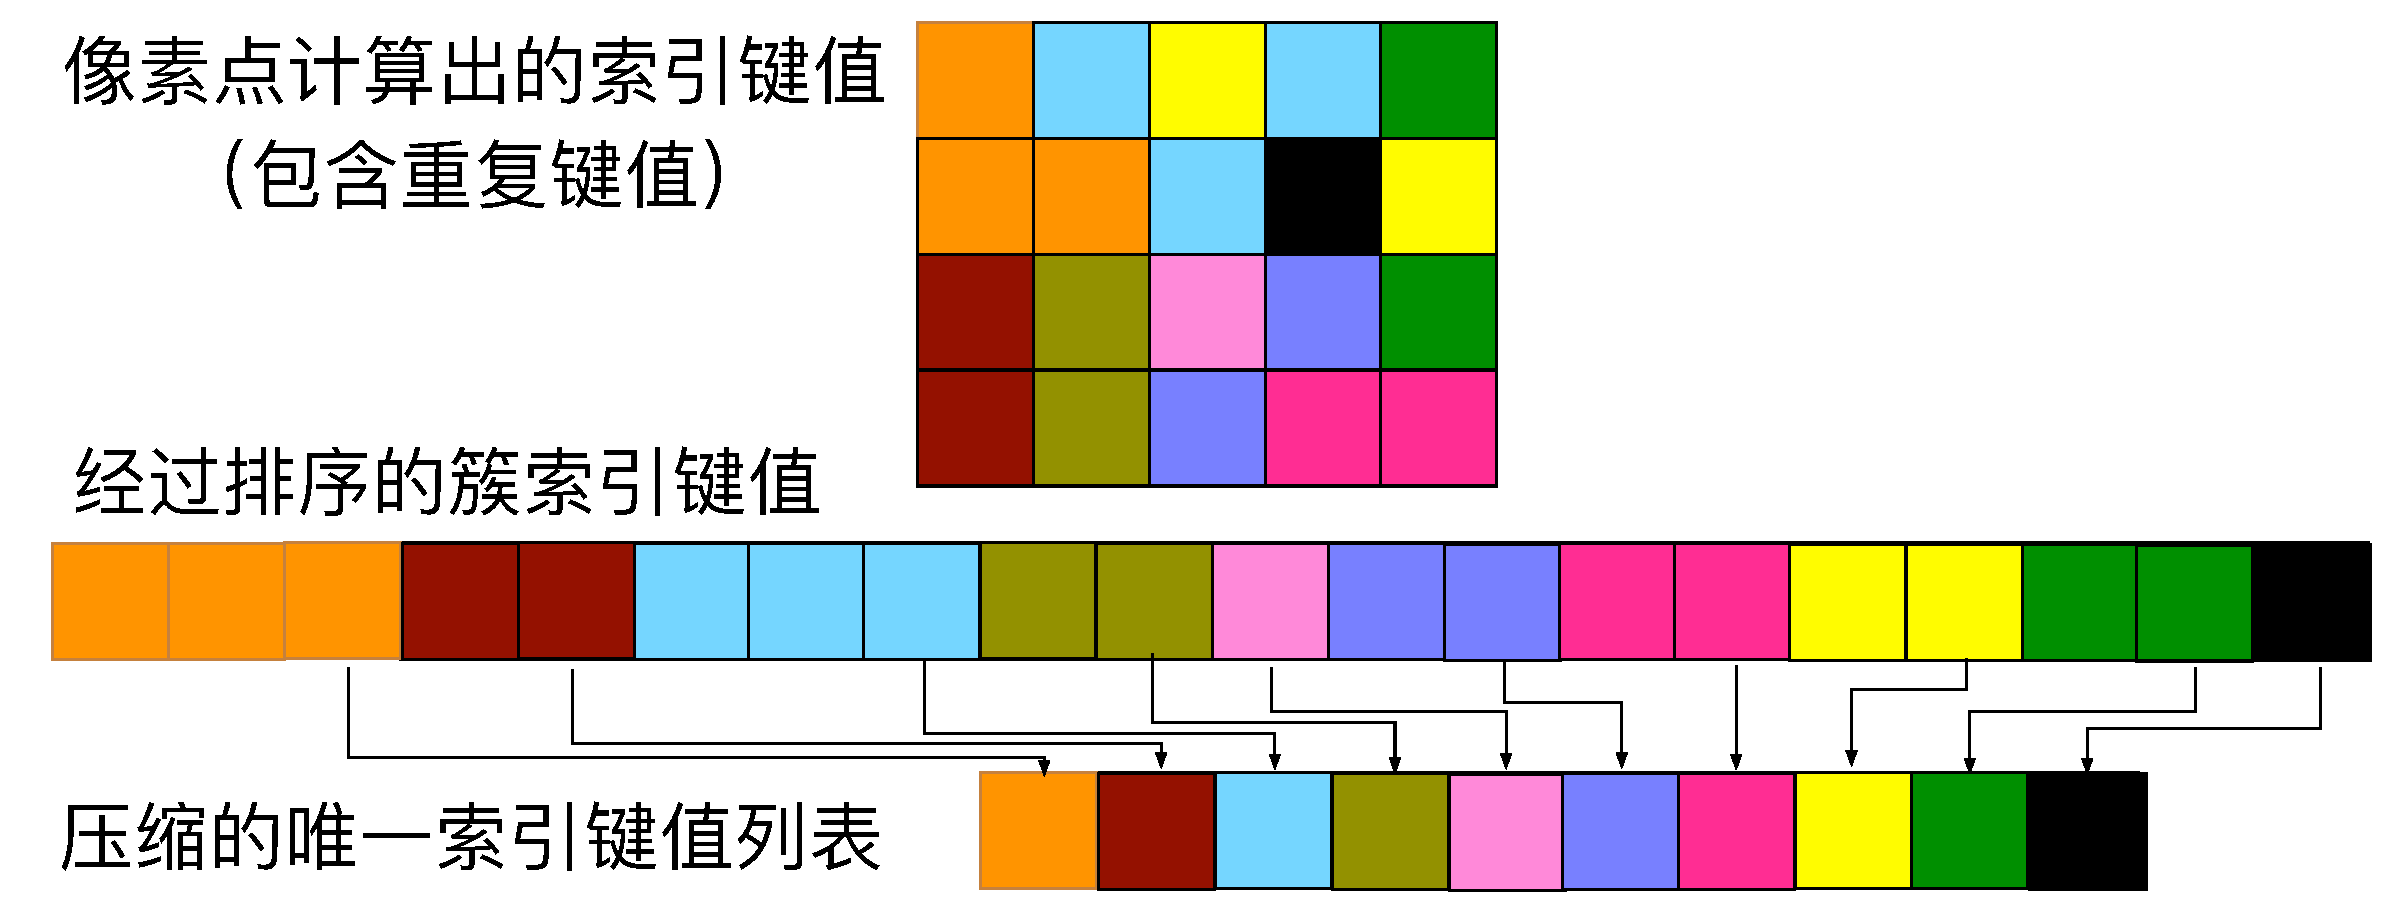
\includegraphics[width=\textwidth]{figures/shade/sorted-key}
\end{center}
	\caption{每个簇内像素的法线分布用一个$3\times 3$的立方体表示,立方体每个面的每个细分面表示一个锥形的法线分布范围,54个位的组合可以由每个像素点分别计算出来。}
	\label{f:shade-sorted-key}
\end{figure}

然而在GPU中进行排序是一件非常影响性能的事情,\cite{a:ClusteredDeferredandForwardShading}的做法是首先以2D屏幕空间的块为单位进行本地排序,由于每个块内的像素点是连续的,并且它是$32\times 32$大小的像素块,所以可以充分利用GPU的并行计算性能,并且每个块内的数据可以写入到本地共享缓存,而不是全局内存进行计算。

另一种方法是使用虚拟纹理\cite{a:VirtualTexturing}(virtual texture)\index{虚拟纹理virtual texture}\index[en]{virtual texture虚拟纹理},虚拟纹理用来存储需要巨大内存的稀疏数据,它可以将一个地址映射到一片紧密的内存区,这样用来降低内存的占用,虚拟内存使用页表(page table)\index{页表page table}\index[en]{page table页表}来映射索引到紧密的物理内存区。然而由于簇索引键值的可能值的范围非常巨大,所以他们使用\cite{a:Glift:GenericEfficientRandom-AccessGPUDataStructures}中的动态分配页表的方法来节省更多的空间,感兴趣的读者可以进一步参考这些论文信息。






\subsubsection{分配光源到簇}
传统的簇光源分配方法是遍历每个簇,然后对每个簇遍历每个光源,进行每光源$-$簇之间的AABB的包围盒相交测试。在这个基础上,\cite{a:ClusteredDeferredandForwardShading}提出首先对所有光源构建一个包围体层次结构(bounding volume hierarchy,BVH)\index{包围体层次结构bounding volume hierarchy,BVH}\index[en]{bounding volume hierarchy,BVH包围体层次结构},以此来加速每个簇内光源的遍历。\cite{a:PracticalClusteredShading}进一步提供了一些加速点光源和聚光灯光源与簇的相交计算,这通过进一步挖掘光源的真实包围几何体而不是一个简单的立方体包围体来减少簇的计算量。

本节我们要介绍的是来自\cite{a:GPUPro7:AdvancedRenderingTechniques}中针对DirectX 12的基于保守光栅化技术的光源分配方法,这是一种利用图形处理器的光栅化技术能够产生非常精确的簇光源分配的方法,当然这种方法仅适用于凸面光源(convex light)\index{凸面光源convex light}\index[en]{convex light凸面光源}形状,考虑到大多数光源如点光源和聚光灯光源的包围体都是凸面的,因此这种方法非常实用。

保守光栅化化(conservative rasterization)\index{保守光栅化化conservative rasterization}\index[en]{conservative rasterization保守光栅化化}的概念非常简单,传统光栅化技术在选择每个图元所覆盖的片元时,是以该图元所占的面积是否覆盖该片元的中心位置来决定该图元是否覆盖到该片元,如图\ref{f:shade-conservative-rasterization}(a)图所示,显然这样的方法运用到光源剔除中就会漏掉一部分光源对簇的影响。与之相对应,保守光栅化则考虑任何部分被图元面积占用的片元均为有效片元,如图\ref{f:shade-conservative-rasterization}(b)图所示。在DirectX 12中,通过在创建一个管线状态对象的时候设置ConservativeRaster的标识为D3D12\_CONSERVATIVE\_RASTERIZATION\_MODE\_ON来开启保守光栅化化\footnote{OpenGL也可以通过一些扩展如GL\_INTEL\_conservative\_rasterization和GL\_NV\_conservative\_raster等来支持保守光栅化。}。

\begin{figure}
	\sidecaption
	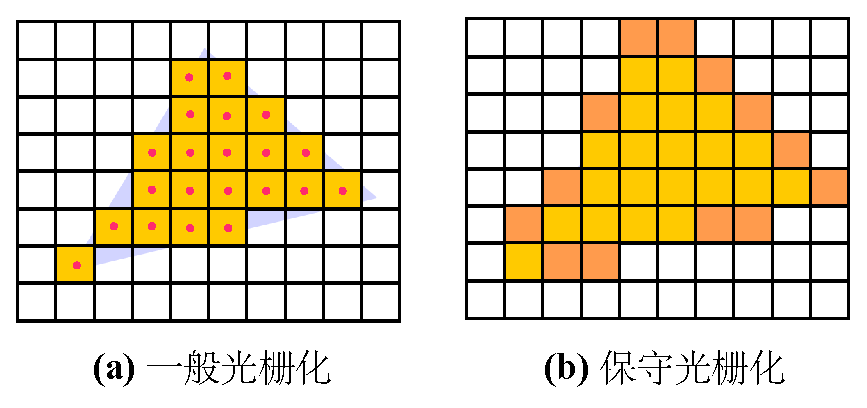
\includegraphics[width=0.6\textwidth]{figures/shade/conservative-rasterization}
	\caption{传统光栅化与保守光栅化的区别,保守光栅化会包含所有图元面积覆盖到任何部分面积的片元。}
	\label{f:shade-conservative-rasterization}
\end{figure}

保守光栅化簇光源分配方法的基本过程可以分为两步,这两步均针对每个光源类型为单位进行:

\begin{enumerate}
	\item 壳通道(shell pass)\index{壳通道shell pass}\index[en]{shell pass壳通道}: 此通道首先将每个光源的包围几何体利用光栅化技术渲染到2D屏幕上以块(tile)为基本单位的分辨率上,并记下每个光源在每个块上的最大和最小深度值。之所以称为壳通道,是因为它找出了每个光源在每个块所在的子视锥体上所占的外形;
	\item 填充通道(fill pass)\index{填充通道fill pass}\index[en]{fill pass填充通道}: 利用壳通道产生的最大最小深度值来填充簇的光源列表。
\end{enumerate}

\begin{figure}
\sidecaption{
	\begin{subfigure}[b]{0.28\textwidth}
		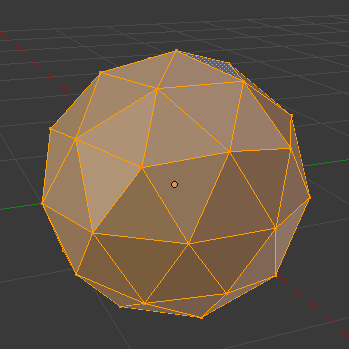
\includegraphics[width=1.\textwidth]{figures/shade/shape-1}
		\caption{42个顶点球行光源}
	\end{subfigure}
	\begin{subfigure}[b]{0.28\textwidth}
		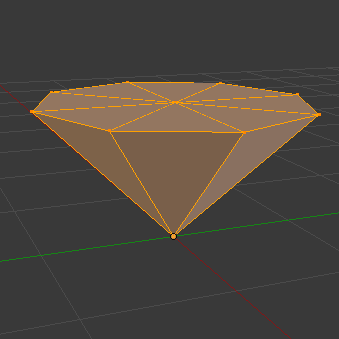
\includegraphics[width=1.\textwidth]{figures/shade/shape-2}
		\caption{10个顶点圆锥形光源}
	\end{subfigure}}
\caption{在保守光栅化光源分配技术中,每个类型的光源使用一个单位网格表述,它们可以在每个实例中使用不同的变换矩阵改变尺寸和位置。}
\label{f:shade-shape}
\end{figure}

由于使用光栅化技术,所以每个光源必须要有一个网格的几何表述,并且该几何表述必须是凸面的,这种几何表述也使得我们可以使用一些不规则的光源类型。需要注意的是,由于场景中的光源数量比较大,所以分别对每个特定的光源实例存储对应的几何数据并不是一个好方法,所以这里仅对每个类型的光源存储一个几何网格数据,并且每个顶点数据在$x-,y-$和$z-$方向上分布被限制到$-1$到1的单位尺寸,如图\ref{f:shade-shape}所示,这样就可以使用图形接口中的实例化渲染,而每个渲染实例在顶点着色器中被变换到其光源的真实尺寸及位置。所以在保守光栅化光源分配方法中,每个通道都是以一个光源类型(而不是每个光源实例)为单位的。






\paragraph{壳通道}
壳通道的主要任务是找出每个光源在屏幕上每个块(tile)内包围簇范围的最大最小深度,例如图\ref{f:shade-tile-shell-pass}所示,由于光源始终是凸面的,只要找出这两个值,则在后面的填充通道则很容易正确地分配每个光源到每个簇内。由于深度方向上簇的数量有限,所有一个R8G8的渲染目标足以存储两个簇的深度值。

\begin{figure}
	\sidecaption
	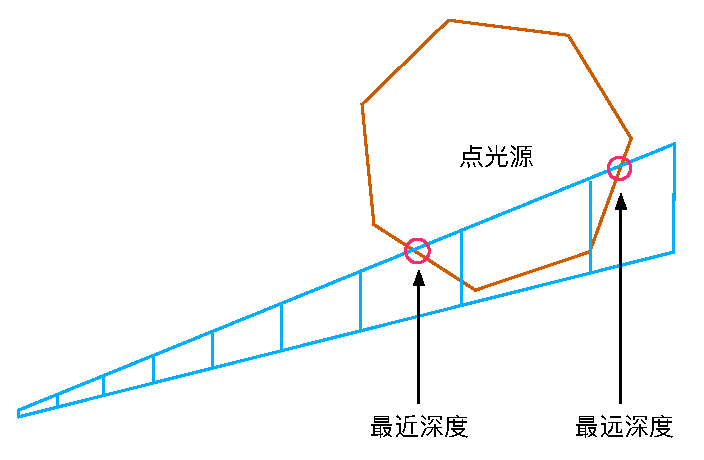
\includegraphics[width=0.6\textwidth]{figures/shade/tile-shell-pass}
	\caption{壳通道的主要任务是找出每个光源在每个块内覆盖的簇的范围,由于光源是凸面的,所有找出最大最小深度方向上的簇之后,该光源就会被分配到该块内最大和最小深度范围以内的所有簇中去}
	\label{f:shade-tile-shell-pass}
\end{figure}

要存储每个光源在每个块上的最大最小深度值,就需要为每个光源设置一个独立的渲染目标,而前面我们已经说明每个通道是以光源类型为单位的,每个光源类型包含多个光源的实例,所以这就要求渲染目标是一个Texture2DArray类型的数组纹理,其数组的数量为每个类型光源对应的光源实例,数组中每个图像的分辨率等于2D屏幕上块的分辨率,如图\ref{f:shade-shell-pass}所示。

\begin{figure}
	\sidecaption
	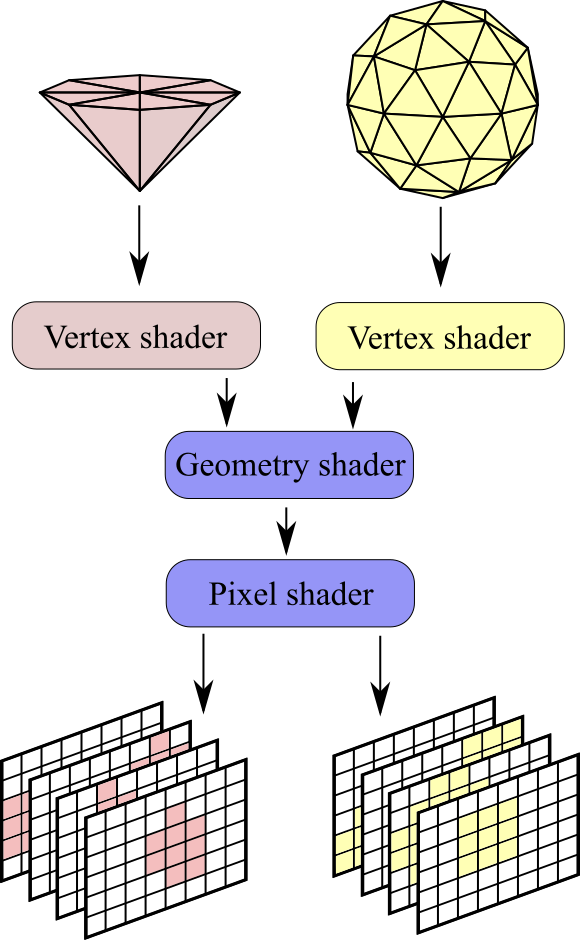
\includegraphics[width=0.5\textwidth]{figures/shade/shell-pass}
	\caption{保守光栅化光源分配方法以光源类型为绘制单位,图中左右两列分别表示聚光灯和点光源两个不同的类型;每个类型的每个光源实例都对应一个渲染目标,所以下边的渲染目标是一个数组纹理,数组纹理的尺寸对应该类型光源实例的数量,每个纹理的分辨率为2D屏幕上块的分辨率;每个光源实例对应的纹理切片的渲染目标在几何着色器中选择}
	\label{f:shade-shell-pass}
\end{figure}

每个光源类型的所有光源实例通过DrawIndexedInstanced实例化渲染命令开始壳通道的绘制,实例的数量则等于场景中该光源类型光源实例的数量,每个光源实例拥有自己的变换矩阵用于将单位网格顶点数据变换到视图空间,顶点着色器根据SV\_InstanceID来分别对每个光源实例的顶点执行变换。

在保守光栅化光源分配方法中,几何着色器必须被使用以设置每个实例的光源被渲染到不同渲染目标中,这通过在几何着色器中设置SV\_RenderTarget\ ArrayIndex到数组纹理中不同的切片来实现。此外,为了后面片元着色器的正确处理,每个片元需要与一个三角形图形进行比较,所以我们需要将三角形的三个顶点输入到片元着色器,同时标识这些顶点变量为nointerpolation,以保证片元着色器中对簇深度的所有计算都是在观察空间的,这是因为有些光源处于视锥体之外的仍要被考虑(例如部分与视锥体相交),如果使用屏幕空间则这部分光源不能够被正确表述。

片元着色器的每个实例对应于屏幕区域一个块,每个块实际上是一个以摄像机为原点,四个面分别穿过块四边的锥形。一旦一个片元着色器实例被执行,说明三角形的至少一部分和该块相交,所以在片元着色器中每个三角形必须与该块对应的锥形进行相交计算。块与三角形进行相交计算时,最大最小深度可能的值的情况如图\ref{f:shade-tile-triangle}所示,圆圈表示最大最小深度值出现的地方,这里算法比较简单,读者可以参考\cite{a:GPUPro7:AdvancedRenderingTechniques}中的算法实现,这里仅讨论思路。

\begin{figure}
	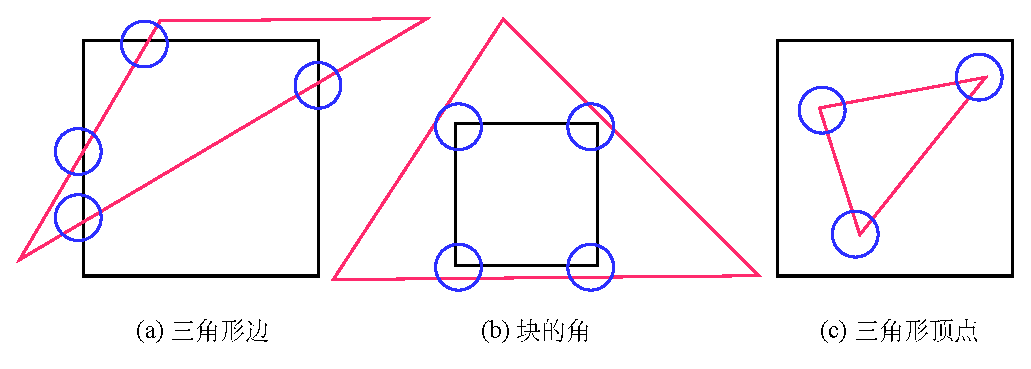
\includegraphics[width=\textwidth]{figures/shade/tile-triangle}
	\caption{块与三角形相交的三种可能的情况,其中(a)发生于三角形的边上,(b)出现在块的四个角,而(c)出现于三角形的三个顶点}
	\label{f:shade-tile-triangle}
\end{figure}

相交计算出的结果根据该三角形面的方向以确定是最大深度或最小深度值,这些深度值在根据簇在深度方向上的指数分布或其他特征求出该簇的索引值\footnote{注意这里的簇索引值可能尽是深度方向上的索引,而不需要存储全局的索引值,这样能够使用更少的数据进行存储,否则16位的R8G8渲染目标根据存储不了全局那么多的簇索引值,后续的填充通道再将其转化为全局簇索引值。},然后将这两个值写入到该光源实例对应的渲染目标上。





\paragraph{填充通道}
有了每个光源在每个块内的最大最小深度值,填充通道直接使用一个计算着色器,它同样以每个光源类型为单位,以块为分辨率,分别根据每个块内每个光源所占的最大最小深度值对其他介于最大最小深度之间的簇进行填充,如图\ref{f:shade-fill-pass}所示,每个计算着色器实例内遍历该实例对应块内所有的簇,只要簇索引值介于最大最小值值之间则对其进行光源分配,这里需要注意的是最大最小值存储的是深度方向的簇索引值,所以需要进行正确地转换。这里计算出的结果将被直接写入到全局的簇光源索引值列表中去,这和分块着色的思路差不多。

\begin{figure}
\begin{center}
	\begin{subfigure}[b]{0.49\textwidth}
		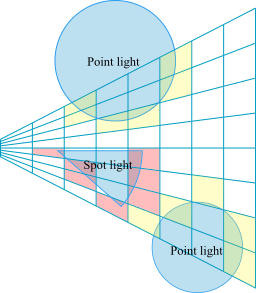
\includegraphics[width=1.\textwidth]{figures/shade/fill-pass-1}
		\caption{壳通道结果}
	\end{subfigure}
	\begin{subfigure}[b]{0.49\textwidth}
		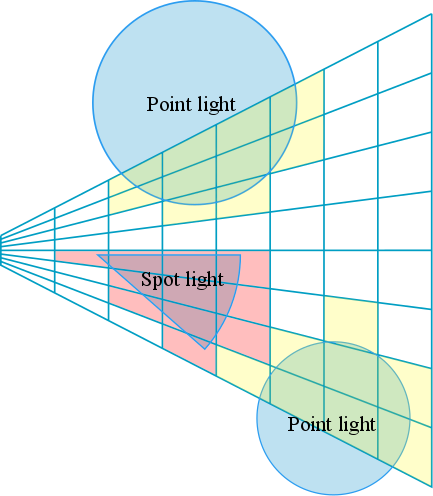
\includegraphics[width=1.\textwidth]{figures/shade/fill-pass-2}
		\caption{填充通道结果}
	\end{subfigure}
\end{center}
\caption{壳通道计算出每个光源在每个块内的最大最小深度值,填充通道就可以利用两个值对每个簇进行光源分配,基于保守光栅化的光源分配方法非常能够非常精确地反应光源的实际几何形状,大大减少了无效的光源分配}
\label{f:shade-fill-pass}
\end{figure}





\subsubsection{着色计算}
分簇着色和分块着色方法在着色计算方面没有太多区别,它同样可以使用于前向或延迟渲染方法中。但由于大大减少了每个簇内光源的数量,因此渲染性能较分块着色得到很大提升,如图\ref{f:shade-cluster-performance}所示。

\begin{figure}
	\sidecaption
	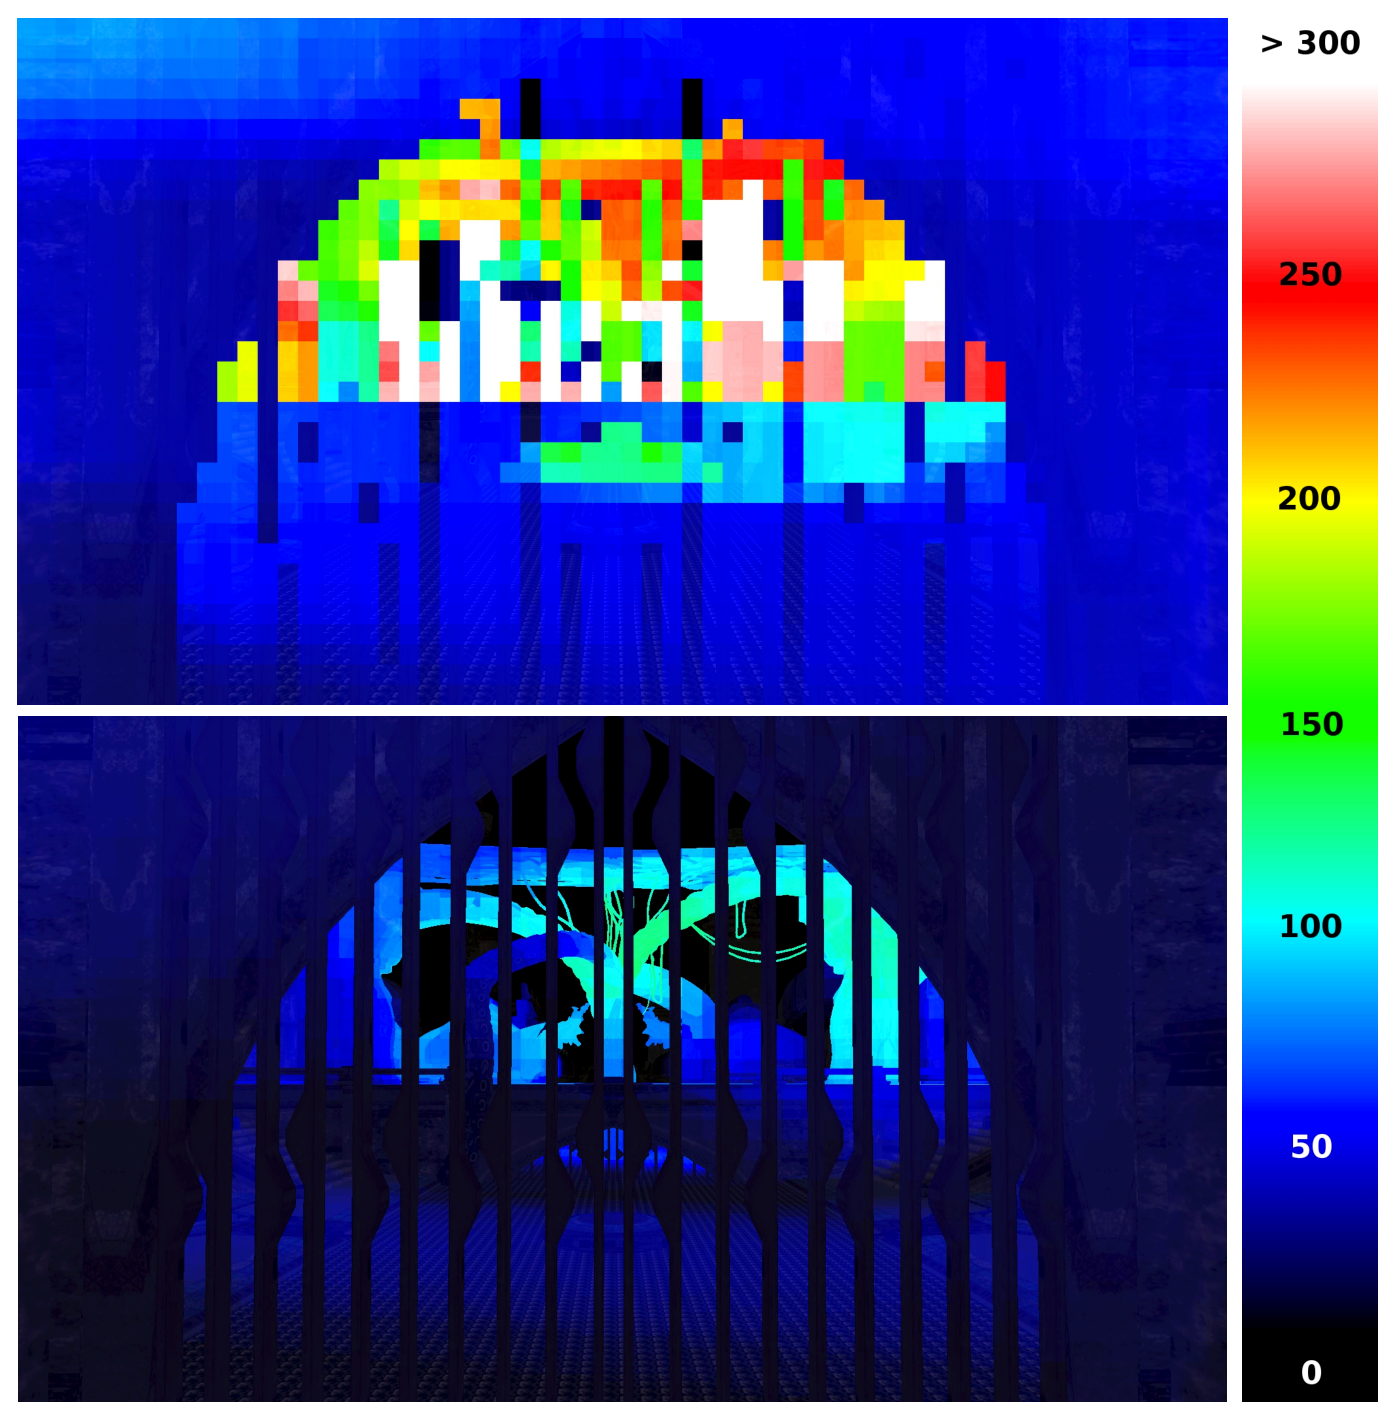
\includegraphics[width=0.6\textwidth]{figures/shade/cluster-performance}
	\caption{图中的颜色表示光源数量,分块着色(上图)和分簇着色(下图)从屏幕的块看上去的光源数量呈现较大的差别,分块着色存在大量的无效光源}
	\label{f:shade-cluster-performance}
\end{figure}

分簇着色更进一步地利用光源的局部性,将每个光源对环境的影响降到最低,从而提供更好的计算性能,从图\ref{f:shade-cluster-performance}我们可以看到分簇着色每个像素计算的光照数量非常低,从而能够轻松应付巨大的光源数量,因为不管光源数量多么巨大,分配到每个簇内的光源数量几乎没有太多变化\footnote{通常场景中的光源都是大致平均分配到整个场景中,现实中很少那种很多光源堆积到一个局部空间的情况。},这只是存在光源分配阶段由于光源数量的增多导致的计算量,因为在整个计算中,只有光源分配部分是和光源数量有较大耦合的。

分簇着色最重大的意义在于,通过这种光源的局部性特征,将场景复杂度完全从光源数量中解脱出来,从而不管场景变得多么复杂,它能始终提供一个稳定的帧率,这是实时渲染技术最重要的权衡指标,因为一个不能保证稳定帧率的技术几乎无法用在实际的产品中。





\section{着色器管理}\label{sec:shade-deferred-custom-shader}
在传统的渲染管线中,渲染是以几何体为单位进行的,相同类型的几何体可以使用对应类型的着色器。但是在延迟着色中,每一次渲染是以屏幕上的一块区域为单位进行着色计算的,这块区域内的像素点可能分别来自不同类型的几何体,它们可能分别具有不同类型的材质参数,所以使用延迟着色,另一个挑战是怎样管理好各种类型物体的着色计算。所幸的是,随着近几年基于物理的渲染模型的广泛使用,如第\ref{chp:intro}章讲述的那些BRDF/BSDF模型,游戏场景中大量的物体表面都可以用比较统一的一些材质参数来表述,剩下仅有一些特殊的物体如毛发,皮肤等使用其他特殊的材质模型。

多种类型的几何体混在一起使用相同的着色器,这就避免不了分支的处理,而GPU中的分支计算可能会对程序性能造成很严重的影响。本节要介绍的是顽皮狗工作室在神秘海域4\cite{a:DeferredLightinginUncharted4}中使用的管理着色器的方案。

\begin{figure}
\begin{fullwidth}
	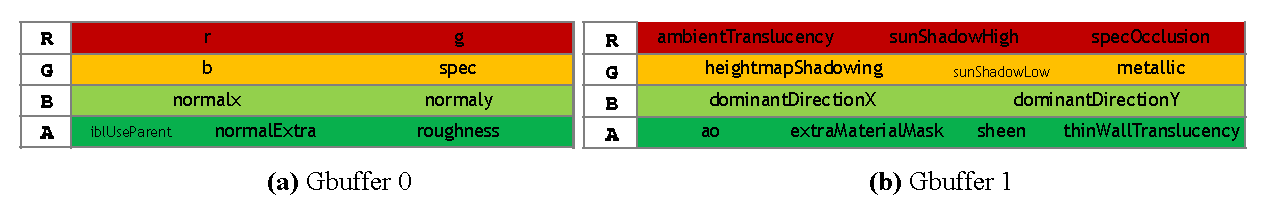
\includegraphics[width=1.0\thewidth]{figures/shade/g-buffer}
	\caption{顽皮狗神秘海域4中使用的基本的两个G-buffer,每个G-buffer中每个像素仅包含16位,它充分使用GCN架构的位解码技术来尽量压缩每个参数的长度(图片数据来自顽皮狗神秘海域4)}
	\label{f:shade-g-buffer}
\end{fullwidth}
\end{figure}

首先,G-buffer必须要支持所有类型的材质参数,每种不同类型的材质需要使用不同的渲染方法,所以这就可能导致巨大的G-buffer,因为其中一些材质参数对另一些类型的物体并不适用。为了尽可能减少G-buffer的体积,他们进行两个方面的优化,首先是对于特殊的材质,他们使用相互独立的材质参数,如图\ref{f:shade-g-buffer}所示,两个基本的G-buffer用来存储所有物体都需要的材质参数,例如法线,位置,粗糙度等等,第三个可选的G-buffer用来存储每种类型特殊的一些材质参数,这些物体包括织物,头发,皮肤以及丝绸等等,这个特殊的G-buffer对每个物体只使用一种类型,例如一个表面不可能同时包含织物和皮肤的材质参数,这是由材质创作管线限制的。

其次,他们充分使用GCN架构内置的的位解码方法来充分压缩每个参数的长度,使得图\ref{f:shade-g-buffer}中每个G-buffer中每个像素仅占用16位的存储空间。传统的着色器编程语言通常使用固定的包含1到4个分量内部图像格式,某些参数在实际中可能占用比一个分量更少的位置,这就会导致一定的浪费。GCN架构提供的解码方法\cite{a:Low-levelShaderOptimizationforNext-GenandDX11}可以对任何整数按位进行解码,这使得我们可以在帧缓存中存储任何长度(甚至超过4个分量)的数据,并且这个操作可以在1个GPU时钟周期内完成,例如以下代码从一个整数中分别获取一个1,5和11位的颜色分量值:

\begin{lstlisting}[language=C++]
int r = s & 0x1F; 			  // 1 cycle
int g = (s >> 5) & 0x3F;	// 1 cycle
int b = (s >> 11) & 0x1F;	// 1 cycle
\end{lstlisting}

在着色器编程中有一个术语叫大型着色器(uber shader),这种着色器往往是将各种材质类型以及光照类型的功能全部写在一个着色器中,这样就导致着色器中会包含大量的分支计算,而通过第\ref{chp:hardware}章中的内容可知,GPU中的分支计算会严重影响其性能,最坏的情况下,每个着色器的每个分支都要被执行一面,尽管有大量的着色器实例的计算是无效的。

然而我们已经说过,由于延迟着色将各种不同类型材质的物体混在一起,这就很难避免大型着色器,这就留给我们似乎也是唯一的方向:那就是我们能不能将这些混在一起的像素点,根据其材质类型将其分离出来,然后对每种类型使用一个独立的渲染通道?

这正是顽皮狗在神秘海域4\cite{a:DeferredLightinginUncharted4}中使用的渲染技术,实际上这也是Battlefield 3\cite{a:SPU-basedDeferredShadingforBattlefield3onPlaystation3}中已经使用过的技术,我们此处以神秘海域4中的内容为准。

神秘海域4中的延迟着色阶段是使用计算着色器以块为单位进行渲染的,其中每个块包含$16\times 16$个像素点。在延迟着色阶段,计算着色器分两步处理块中像素的着色计算:

\begin{enumerate}
	\item 对每个块执行材质类型定义(material classification)。
	\item 对每个材质类型分别执行一次计算着色器。
\end{enumerate}

材质定义阶段的目的是找出每个块使用的计算着色器类型。为此,他们对每个不同材质类型的组合建立一个单独的计算着色器通道,所有可能的材质类型组合存储在一个查询表(lookup table)中,这样每个块通过其材质组合的索引值就能找到对应的计算着色器,如果在材质类型定义阶段像这样区分了所有的像素点,第二阶段就可以对每个材质类型组合使用一个独立的计算着色器,其仅包含少量\footnote{由下面的内容可知,这个数量取决于该块内材质类型的数量,在一个局部的块内,大部分的材质类型都是相同的,即使具有不同类型的材质,其分支的数量也比一个大型着色器的分支要少得多。}甚至无分支计算。

那每个块怎样计算这个材质类型组合的索引值呢?他们称这个材质类型组合的值为一个块的材质ID\footnote{注意,这里材质ID的概念是针对块的,而不是针对一个物体。由于块包含多个像素点,所以材质ID是一个材质的组合,而不是只单个材质。这里可以理解为,每个物体本身包含的材质是基本的原子的着色类型(由于他们假设所有材质相互独立),而材质ID是由于一个块包含多个原子功能之后总的看起来的着色类型。}(material ID)\index{材质IDmaterial ID}\index[en]{material ID材质ID}的属性,它实际上是一个位平面,每个位代表一个着色器特性(shader feature),或者我们可以称为着色器中计算功能的原理单位(其内部不包含分支的),神秘海域4中的材质ID使用12位来表示,由于这些材质类型之间是相互独立的,所以其可以被压缩到8位进行存储。

由于材质ID是一个位平面,所以每个块内的材质ID可以通过其内每个像素点材质对应位的或操作得来,然后我们就可以通过这个材质ID从查询表中查询到该块计算着色器的类型,将这个信息保存起来,就可以在后续的阶段被使用相应的计算着色器正确执行,材质类型定义阶段的代码如下:

\begin{lstlisting}[language=C++]
uint materialMask = DecompressMaterialMask(materialMaskBuffer.Load(int3(screenCoord, 0)));

uint orReducedMaskBits;
ReduceMaterialMask(materialMask, groupIndex, orReducedMaskBits);

short shaderIndex = shaderTable[orReducedMaskBits];

if (groupIndex == 0)
{
	uint tileIndex=AtomicIncrement(shaderGdsOffsets[permutationIndex]);
	tileBuffers[shaderIndex][tileIndex]=groupId.x|(groupId.y<<16);
}
\end{lstlisting}

这里的shaderTable就是材质类型组合的查询表,它表示的是所有可能的包含各组材质组合的着色器,它可以根据材质ID返回表示一个独立的计算着色器的索引值shaderIndex。groupId是每个块的坐标值,每个块会被添加到一个全局的管理所有块材质ID的缓存对象tileBuffers中,后续的着色阶段就会分别根据每个shaderIndex对被添加到给着色器类型的所有块进行着色计算。

由于这里使用计算着色器以块为单位进行材质类型定义的工作,所以AtomicIncrement表示一个被申领的块,这是一个原理计算器,它保证每个计算着色器实例不会处理同一个块,这里的思路是和\cite{a:SPU-basedDeferredShadingforBattlefield3onPlaystation3}中相似的。

由于一个块包含$16\times 16$个像素,所以块内每个像素仍然可能使用不同的材质类型或组合,这就导致每个计算着色器内部还是会存在分支处理,尽管它比大型着色器的分支数量要小得多。这里进一步的优化是将那些块内每个像素拥有完全一样材质类型组合的块使用的着色器的分支计算去掉,所以这里使用了一个额外的包含无分支排列组合的查询表(branchless permutation table)\index{无分支组合查询表branchless permutation table}\index[en]{branchless permutation table无分支组合查询表}。我们可以使用下面的语句修改上述第6行代码为:

\begin{lstlisting}[language=C++]
bool constantTileValue = IsTileConstantValue( … );
short shaderIndex = constantTileValue? branchlessShaderTable[orReducedMaskBits]: shaderTable[orReducedMaskBits];
\end{lstlisting}

相对于传统的大型着色器,神秘海域4中使用的着色器管理技术可以带来$20\%\sim 30\%$的性能提升,如图\ref{f:shade-material-ID}所示,场景中大部分块内每个像素都拥有相同的材质类型组合,即它们不包含分支处理,将这些分支去掉,以及以材质类型为单位减少大型着色器的分支处理,延迟着色的性能得到大大提升。

\begin{figure}
	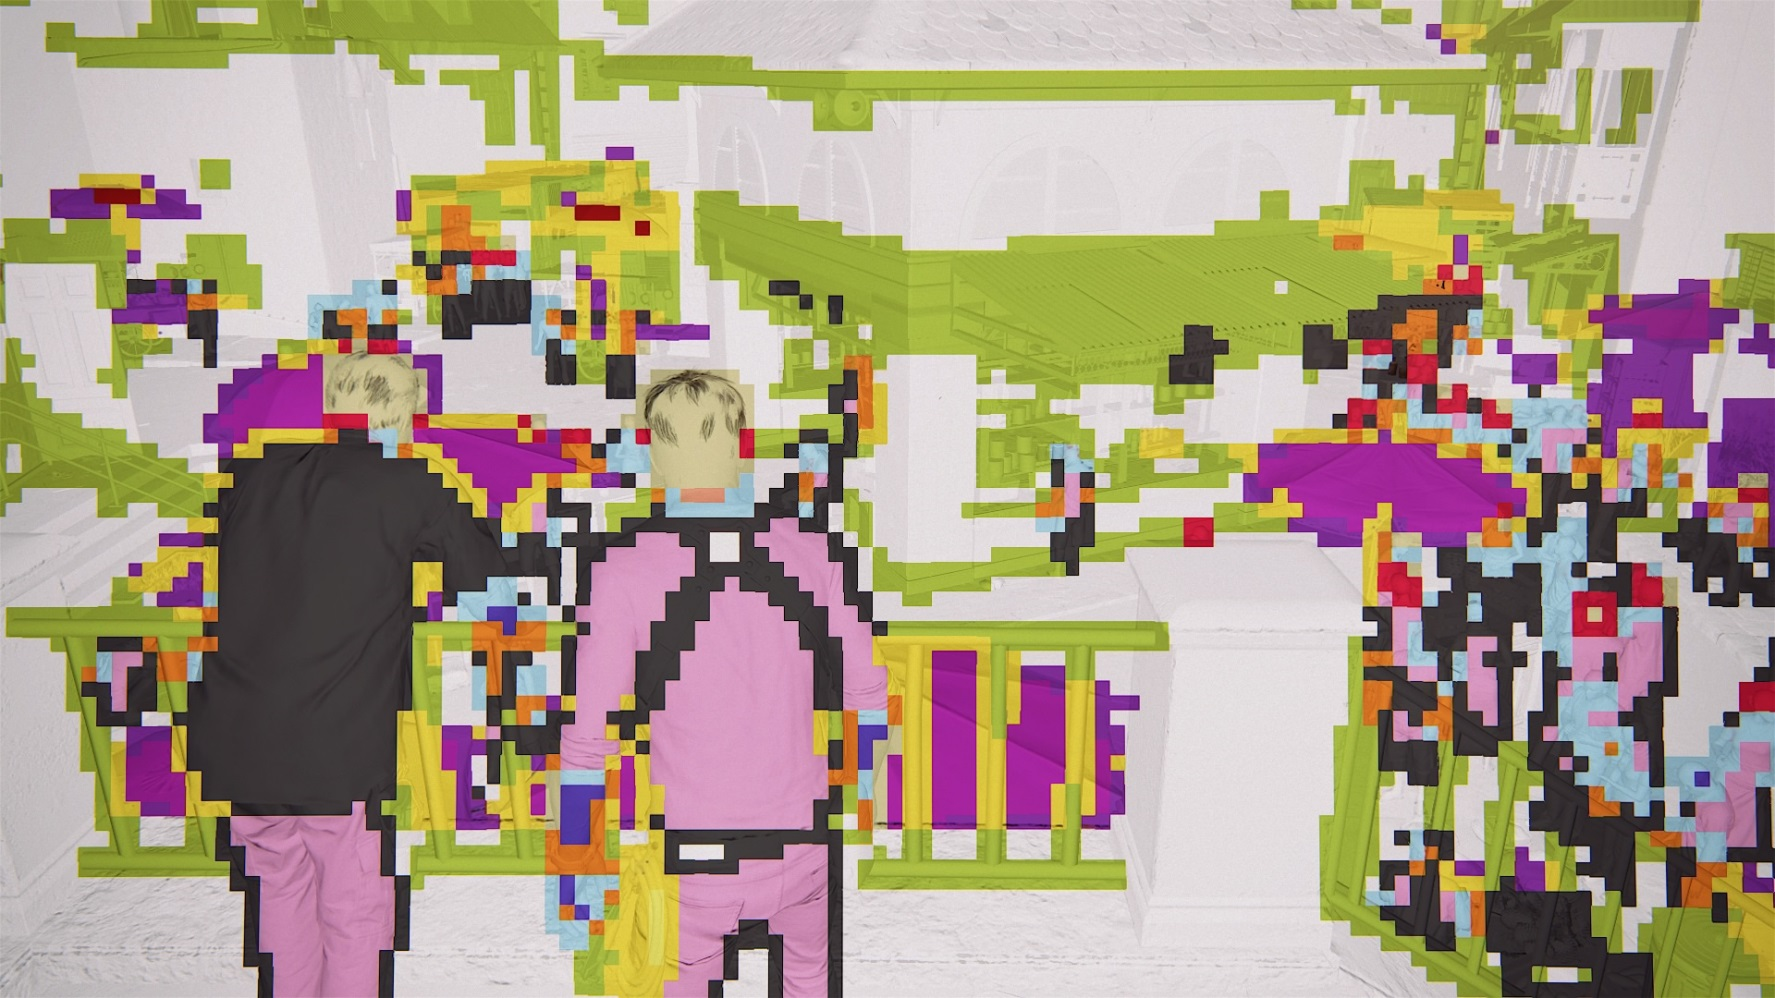
\includegraphics[width=1.0\textwidth]{figures/shade/material-ID}
	\caption{图中每个颜色代表不同的材质ID,它们分别使用具有较少分支甚至无分支的着色器(图片来自顽皮狗工作室)}
	\label{f:shade-material-ID}
\end{figure}

另外,所有这些着色器的分配工作都是由游戏引擎工具自动完成,例如完成不同材质类型组合着色器的编译,以及不同块之间按材质ID进行划分都是对美术师透明的,这大大简化了对物体着色的流程以及渲染的灵活性,并大幅提升了渲染性能。同时,添加新的材质类型并不会影响到着色器管理的复杂度。





\section{延迟着色中的反走样技术}\label{sec:shade-anti-aliasing}
我们在第1章介绍了对数字信号采样的基础知识,以及走样的概念,并在第\ref{sec:intro-msaa}节简要介绍了图形学渲染领域的两种基本全屏反走样技术:超采样反走样和多重采样反走样,本节我们将深入介绍全屏反走样的一些流行技术。

首先我们回顾一下走样(aliasing)\index{走样aliasing}\index[en]{aliasing走样}及反走样(anti-aliasing,AA)\index{反走样anti-aliasing}\index[en]{anti-aliasing反走样}的基本概念。一个连续信号在被采样为离散信号时,只有在其对应的频率域(frequency domain)\index{频率域frequency domain}\index[en]{frequency domain频率域}上,使用能够覆盖2倍及以上的频率带宽(frequency bandwith)\index{频率带宽frequency bandwith}\index[en]{frequency bandwith频率带宽}的采样率(sample rate)时,离散信号才能被完美重建(reconstruction)为原始连续信号,否则重建后的原始信号将会发生走样,由于一些高频信号被“削平”了,许多原本不同的信号看起来像相同的信号(一些信号像另一些信号的别名)。由于在场景中,几何物体的边缘周围的颜色频率域变化非常大,基本上一般的屏幕分辨率根本无法捕捉这些频率域的变化范围,所以走样几乎不可避免。另一些图形学中的走样发生于着色器中对高频(如高光)函数进行采样,更多的信息详见第\ref{chp:intro}章第\ref{sec:intro-sampling}节的内容。

\begin{shaded*}
	关于aliasing,国内有多种翻译:锯齿,混淆和走样。alias在英语中表示“别名”的意思,可以是正确(例如小名)或错误(例如间谍冒充别人)的别名,aliasing是采样不足导致的多个信号之间无法区分(其中一个像另一个的别名)的现象,只有在图形学中以单个值表示一个像素块的值时才表现为锯齿,锯齿对应的词通常为jaggies。aliasing是可以减弱的,而jaggies是不可消除的,anti-aliasing之后的图像放大之后仍然有锯齿,但是这些信号之间的过度更平滑,所以笔者认为“走样”的翻译更精确一些,而混淆太语义化了,不利于理解概念。
\end{shaded*}

在图形学中主要有两大类走样类型: 其一是由于对空间域的信号采样不足导致的走样,这些称为空间走样(spatial aliasing)\index{空间走样spatial aliasing}\index[en]{spatial aliasing空间走样},它包括几何走样(geometry aliasing)\index{几何走样geometry aliasing}\index[en]{geometry aliasing几何走样},着色走样(shader aliasing)\index{着色走样shader aliasing}\index[en]{shader aliasing着色走样}等,空间走样对应的反走样技术称为空间反走样(spatial anti-aliasing)\index{空间反走样spatial anti-aliasing}\index[en]{spatial anti-aliasing空间反走样},相应使用的过滤器称为空间过滤器(spatial filter)\index{空间过滤器spatial filter}\index[en]{spatial filter空间过滤器};另一种走样是由于帧率的限制,导致对相邻时间内信号的采样不足导致的走样,称为时间走样(temporal aliasing)\index{时间走样temporal aliasing}\index[en]{temporal aliasing时间走样},对应的反走样及过滤器称为时间反走样(temporal anti-aliasing)\index{时间反走样temporal anti-aliasing}\index[en]{temporal anti-aliasing时间反走样}和时间过滤器(temporal filter)\index{时间过滤器temporal filter}\index[en]{temporal filter时间过滤器}。

在图形学中,空间走样的黄金标准是全屏超采样(supersampling)\index{超采样supersampling}\index[en]{supersampling超采样}技术,它直接使用更高的分辨率对场景进行渲染,然后对这种高分辨率的渲染结果进行过滤以“缩放到”屏幕分辨率,使用超采样进行反走样的计算称为超采样反走样(supersample anti-aliasing,SSAA)\index{超采样反走样supersample anti-aliasing}\index[en]{supersample anti-aliasing超采样反走样}或全屏反走样(full-screen anti-aliasing,FSAA)\index{全屏反走样full-screen anti-aliasing}\index[en]{full-screen anti-aliasing全屏反走样}。

由于渲染中使用的着色计算可能非常复杂,而考虑到屏幕中最主要的走样类型为几何走样,因此多重采样(multisampling)\index{多重采样multisampling}\index[en]{multisampling多重采样}技术将几何可见性和着色计算分开,它对几何可见性函数的采样使用类似超采样一样更高的分辨率进行采样,但是每个像素点内只做一次着色计算,并使用可见性的覆盖率作为比率来混合当前的颜色值,这样的反走样技术称为多重采样反走样(multisample anti-aliasing,MSAA)\index{多重采样反走样multisample anti-aliasing}\index[en]{multisample anti-aliasing,MSAA多重采样反走样}。MSAA将每个像素点的着色计算结果分别复制到每个子采样点,所以它使用和SSAA一样大小的存储空间,但是计算量大大降低,不过缺点是不能处理着色走样。

然而MSAA并不适用于延迟着色,因为它会自动将片元着色器输出的结果拷贝多次,这使得本身就非常大的G-buffer更要使用多几倍的存储空间,这又大大增加了延迟着色计算中的带宽占用,因为每个像素要读取多几倍的数据。

另一方面,即使G-buffer的存储和带宽都不是问题,由于MSAA着重于解决几何走样,它仍然无法解决着色器走样。而现代游戏引擎大都使用基于物理的渲染管线,着色器中对函数的采样不足导致的高光部分的走样特别明显,这使得我们必须寻找新的更有效的反走样计算。

本节我们将讨论三种被广泛用在延迟着色中的反走样技术,这三种技术几乎也是目前工业中最流行的反走样技术,它们分别使用几乎完全不同的思路和原理进行反走样处理。




\subsection{形态反走样}
SSAA和MSAA都是在一个像素正方形区域内使用多个采样点(sub sample),每个子采样点形成的区域称为一个子像素(subpixel),如图\ref{f:shade-subpixel}所示,最后再使用某种过滤器对像素中心位置周围的子像素进行过滤,例如一个盒式过滤器(box filter)\myindex{一个盒式过滤器}{box filter}就是求这些子像素颜色的平均值。

\begin{figure}
	\sidecaption
	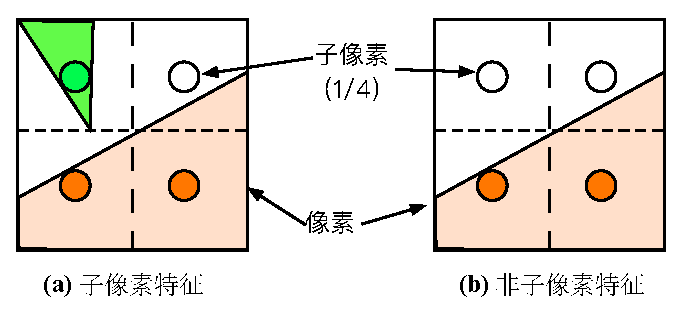
\includegraphics[width=0.65\textwidth]{figures/shade/subpixel}
	\caption{传统的全屏反走样技术对一个像素使用多个子采样点,通过以某种过滤方式计算这些子像素点的权重(例如面积覆盖率,距离等)来实现全屏反走样}
	\label{f:shade-subpixel}
\end{figure}

如果每个子像素具有不同的颜色值,这称为具有子像素特征(subpixel feature)\index{子像素特征subpixel feature}\index[en]{subpixel feature子像素特征},则SSAA能够比较准确地反应这种子像素特征,如图\ref{f:shade-subpixel}(a)所示;然而,如果不考虑子像素特征,即每个像素只有一个颜色值,那么子像素的作用仅是用来计算该像素的覆盖率,这正是MSAA的思路,如图\ref{f:shade-subpixel}(b)的思路。

通常人眼对于物体形状以及颜色变化(color variation)\index{颜色变化color variation}\index[en]{color variation颜色变化}最敏感,而在渲染结果中这种变化通常来源于几何体的轮廓(silhouette)\index{轮廓silhouette}\index[en]{silhouette轮廓},要么是深度不连续(depth discontinuities)\index{深度不连续depth discontinuities}\index[en]{depth discontinuities深度不连续},或者是不同物体之间颜色不连续(color discontinuities)\index{颜色不连续color discontinuities}\index[en]{color discontinuities颜色不连续},所以即使不具备子像素特征,MSAA在游戏中运用仍然非常广泛。由于MSAA不适用于延迟渲染,如果我们能够以一种低成本的方式计算出这些轮廓上像素的覆盖率,那么我们就可以做到和MSAA类似的品质。

形态反走样\cite{a:MorphologicalAntialiasing}(morphological anti-aliasing,MLAA)\index{形态反走样morphological anti-aliasing}\index[en]{morphological anti-aliasing形态反走样}正是基于这样的思路,它的核心算法是找出物体的轮廓信息,并利用这些轮廓信息(而不是使用更多的采样点)计算出处于轮廓上像素的覆盖率,然后使用一个后期处理(post-processing)\index{后期处理post-processing}\index[en]{post-processing后期处理}阶段对轮廓上的像素与相邻像素的颜色进行混合。

MLAA基本算法的过程主要包括三个步骤,这里首先简要介绍这三个步骤,后面要讨论的MLAA的一些变体基本上也是按照这三个步骤来进行的,只是每个步骤内部可能使用不同的方法。这三个步骤分别是:

\begin{enumerate}
	\item 根据一定的像素属性(如颜色,深度,法线,几何体ID等)找出图像中不连续的像素,并标记出这些像素中的哪些边处于轮廓边缘,这称为边缘检测(edge detecting)\index{边沿检测edge detecting}\index[en]{edge detecting边沿检测},如图\ref{f:shade-mlaa}(a)中的绿色线段。
	\item 利用这些边缘线段的几何特征计算每个像素与周围邻近用来进行混合的像素的权重值(即是面积覆盖率),如图\ref{f:shade-mlaa}(c)所示。
	\item 对周围邻近的像素按照混合权重进行混合计算求出轮廓上像素的颜色值,如图\ref{f:shade-mlaa}(c)所示。
\end{enumerate}

\begin{figure}
\begin{fullwidth}
	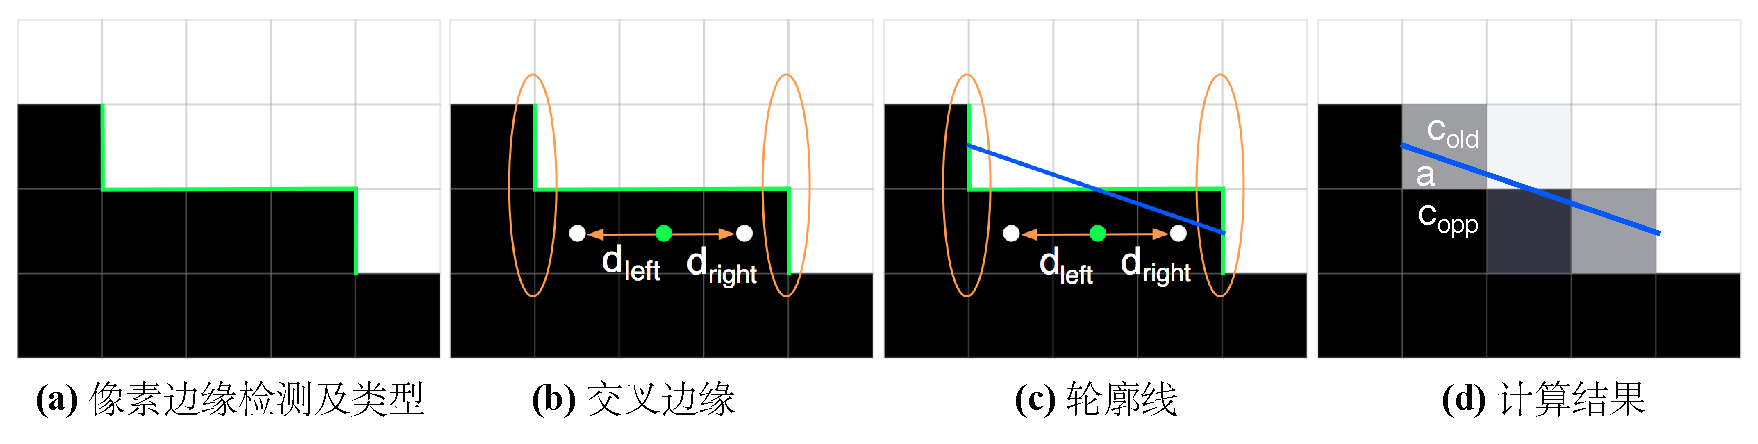
\includegraphics[width=1.0\thewidth]{figures/shade/mlaa-09}
	\caption{MLAA算法首先根据一定的标准标注出图像中不连续的边,并对其划分为L,U以及Z三种类型,然后针对这三种类型的线段连接成分段线性(piecewise-linear)\index{分段线性piecewise-linear}\index[en]{piecewise-linear分段线性}的线段,这些线段将边缘部分的像素分割成两个梯形,其梯形的面积分别代表周围邻近的像素颜色进行混合的权重}
	\label{f:shade-mlaa}
\end{fullwidth}
\end{figure}

由于MLAA是通过后期处理的方式来实现反走样的,所以它的输入就是光栅化渲染的一张屏幕分辨率大小的图像,如图\ref{f:shade-mlaa}(a)所示,在这个图像中,几何体边缘部分的像素完全按照其像素中心位置是否被一个几何体覆盖来对其进行着色计算的,它是一个走样的图像(aliased image)\index{走样的图像aliased image}\index[en]{aliased image走样的图像}。

MLAA拿到图像后第一步需要做的事情是边缘检测,一个图像中的边缘可以通过多种类型的属性来判断,例如相邻像素深度,颜色,法线或者材质等的不连续。通常使用颜色变化来判断边缘,因为通常具有相似颜色的像素更容易聚集在一起,一些实现也使用亮度来计算边缘。

当我们选定了边缘检测的标准之后,边缘检测可以通过遍历图像中的每两个相邻的列和行的像素,并比较相邻像素的值来判断它们的邻边是否处于边缘,如图\ref{f:shade-mlaa}(a)中的绿色线段。因为一条直线段可能包括多个像素的边,所以接下来我们需要找到每条直线段的起点和终点,如图\ref{f:shade-mlaa}(a)所示,由于这些终点的线段与该计算的直线段是交叉垂直的,所以起点和终点线段又称为交叉边缘(crossing edges)\index{交叉边缘crossing edges}\index[en]{crossing edges交叉边缘}。

这些边缘线段可以被划分为三种类型:L,Z以及U型,如图\ref{f:shade-edge-types}所示,每种类型的交叉边缘只包含一个像素的长度,非交叉边缘可以具有任意长度。当这些类型被划分之后,直接连接每个类型的交叉边缘的中点就构成一条轮廓线(silhouette)\index{轮廓silhouette}\index[en]{silhouette轮廓},如图\ref{f:shade-mlaa}(c)中蓝色的线段,它是一个Z-形状交叉边缘的中点链接起来的线段。

\begin{figure}
	\sidecaption
	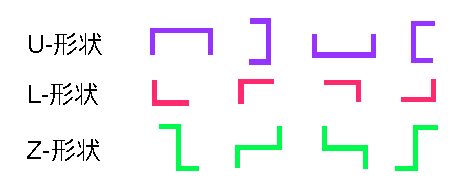
\includegraphics[width=0.45\textwidth]{figures/shade/edge-types}
	\caption{MLAA中的边缘线段被划分为三种类型,每种类型的最短边只包含一个像素的长度}
	\label{f:shade-edge-types}
\end{figure}

当轮廓线段被连接起来以后,它们将轮廓上的像素分割成两个梯形,其每个梯形的面积就代表了该像素与附近像素的颜色用来进行混合计算的权重,我们可以根据边缘线段中$d_{\rm left}+d_{\rm right}$的长度,如图\ref{f:shade-mlaa}(c)所示,以及宽度(一个像素的大小)来计算每个梯形的面积。如图\ref{f:shade-mlaa}(d)所示,$c_{old}$轮廓上像素原来的颜色,$c_{opp}$代表邻近像素的颜色,$a$代表轮廓上的像素的混合权重,则该轮廓上像素的新的颜色值为:

\begin{equation}
	c_{new}=(1-a)\cdot c_{old}+a\cdot c_{opp}
\end{equation}

以上内容讨论了形态反走样方法的基本思路,然而我们并没有说明具体的算法内容,这是因为原始的MLAA算法是针对基于CPU的光线追踪渲染器实现的,现代实时渲染程序主要是面向GPU的,所以我们将在后面的内容详细讨论一个基于GPU的实现方案,即SMAA。

MLAA算法各个阶段的视觉效果如图\ref{f:shade-mlaa-1}所示,它是一种非常高效的反走样技术,在不需要多重采样或超采样的基础下,几乎可以达到4倍于MSAA的效果。并且MLAA是一种后处理算法,它可以被很灵活地加入到任何渲染器而不需要对应的渲染管线做出修改。自从MLAA被提出之后,由于其高效的性能引起了大量的兴趣,在随后的几年大量的MLAA变体算法被提出,例如SRAA\cite{a:SubpixelReconstructionAntialiasingforDeferredShading},FXAA\cite{a:FXAA}等, 读者可以阅读\cite{a:FilteringApproachesforReal-TimeAnti-Aliasing}了解更多详细内容

\begin{figure}
\sidecaption
	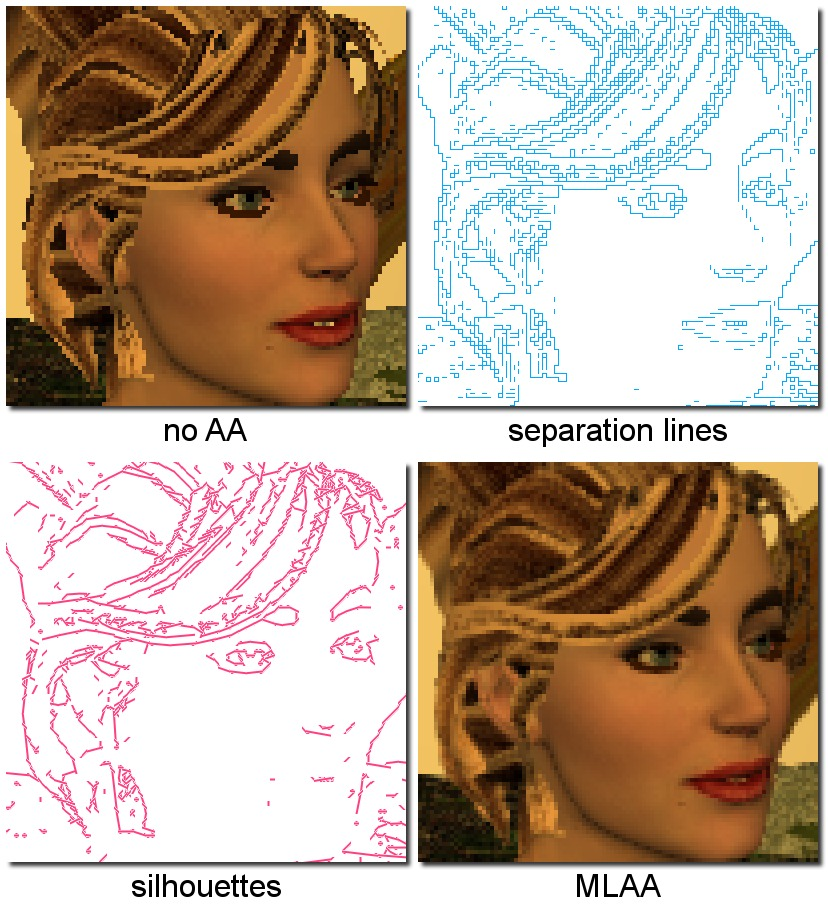
\includegraphics[width=0.65\textwidth]{figures/shade/mlaa-1}
	\caption{左上为MLAA算法输入走样的原图,右上首先根据某种标准计算像素边缘线段,然后根据这些边缘线段连接成左下图对应的轮廓线段,这些轮廓线段将边缘的像素切割成两个梯形,每个梯形的面积则用来表示周围相邻像素用来进行混合计算的权重,最终MLAA计算的结构如右下图}
	\label{f:shade-mlaa-1}
\end{figure}

然而,MLAA的主要缺点是不能处理子像素级的特性,任何小于一个像素的几何体(例如超薄表面,文字等)将不能被有效地处理,由于采样的不足,高光和着色走样也不容易处理;另外,MLAA原始算法主要设计为处理贴近水平或垂直的轮廓,它几乎忽略掉了对角线轮廓,因为对角线轮廓需要考虑更多的像素,而MLAA仅考虑轮廓线上的像素的混合。下面我们将介绍这些变体中由Jimenez等提出的SMAA算法,SMAA是基于GPU实现的,它包含了针对GPU硬件的一些优化,从功能和性能上都具有较大的提升。






\subsubsection{子像素形态反走样}
子像素形态反走样(subpixel morphological anti-aliasing,SMAA)\index{子像素形态反走样subpixel morphological anti-aliasing}\index[en]{subpixel morphological anti-aliasing子像素形态反走样}\cite{a:SMAA:EnhancedSubpixelMorphologicalAntialiasing}是基于Jimenez等于2011年实现的MLAA\cite{a:PracticalMorphologicalAnti-Aliasing}变体的增强算法,本节将放在一起讨论它们。此外,SMAA还包括对于时间反走样的优化,我们将把这部分内容放入到下一节当中,SMAA还被集成到了CryEngine 3\cite{a:Anti-AliasingMethodsinCryENGINE3}当中,读者还可以获取全部SMAA实现的源代码\footnote{可从以下网站获得:\url{http://iryoku.com/smaa/}}。

SMAA和MLAA算法使用相似的步骤,但是每个步骤内部使用的方法是完全不同的。SMAA算法包含三个渲染通道(pass):

\begin{itemize}
	\item 第一通道:首先边缘被检测出来,这些边缘被存储到一个边缘纹理(edges texture)中,如图\ref{f:shade-smaa}(d)所示,纹理中的颜色表示每个边缘在像素中(即上,下,左和右)的位置:绿色像素的边缘在其像素顶部,红色像素的边缘在左边,黄色像素同时在以上两个方向拥有边缘\footnote{出于性能考虑,这里仅存储顶部和左边的边缘,因为其他两边的边缘能够从旁边邻近的像素推导出来。}。此外,在此通道,边缘像素的模板值被记录,以便后续的通道仅处理轮廓上的像素。
	\item 第二通道:计算每个轮廓上像素的混合权重,即是图\ref{f:shade-mlaa}下图中a的值,如图\ref{f:shade-smaa}(e)所示。为了计算该权重值,首先找出每条经过该像素左边和顶部边缘线段的模式,如图\ref{f:shade-smaa}(b)所示,然后计算出该像素距离这些模式线段交叉边缘的距离,然后这两个距离值作为纹理坐标到一个预计算的纹理中进行采样,这个预计算的纹理是根据线段模式计算出来的权重分布值,如图\ref{f:shade-smaa}(c)所示。
	\item 第三通道:根据上一步的权重值从周围的四个像素中取出颜色值进行混合计算,计算结果如图\ref{f:shade-smaa}(f)所示。
\end{itemize}

\begin{figure}
\begin{fullwidth}
	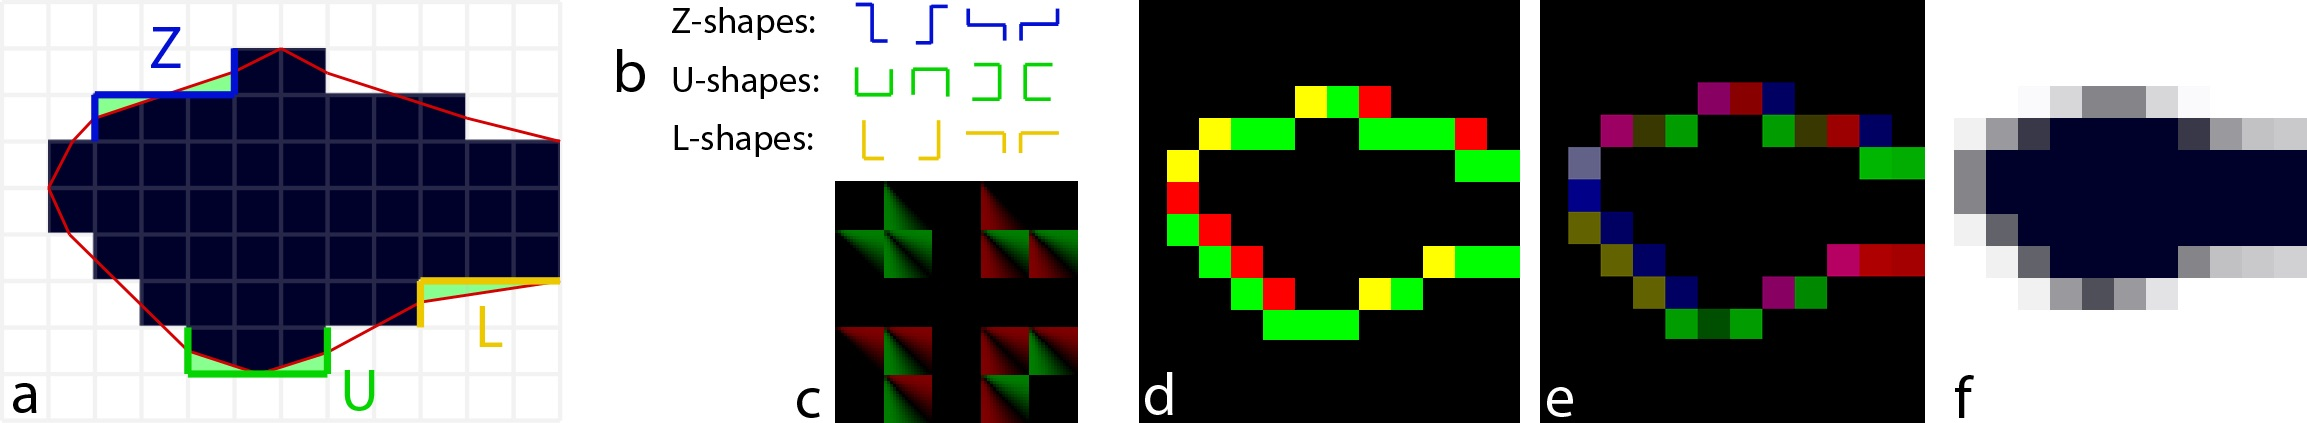
\includegraphics[width=1.0\thewidth]{figures/shade/smaa}
	\caption{MLAA概述: (a)输入的走样的图像,其中红色线段表示轮廓边缘,绿色部分表示覆盖面积,并标注了L,U和Z三种线段模式;(b)原始MLAA算法中预定义的线段模式;(c) Jimenez等MLAA变体中预计算的面积纹理;(d)检测出的边缘; (e)计算出的面积覆盖率;(f) 最终混合结果}
	\label{f:shade-smaa}
\end{fullwidth}
\end{figure}

以下分别详述每个渲染通道内的一些关键处理,SMAA算法的较大特点是充分利用了GPU纹理过滤的功能以大大减少了一些迭代,循环的操作,这些技巧对于着色器编程有非常大的借鉴作用。





\paragraph{边缘检测}\index{边缘检测edge detecting}\index[en]{edge detecting边缘检测}
为了进行边缘检测,首先要选择用于相邻像素边缘比较的量,例如RGB颜色,亮度,深度,法线,几何体ID等,SMAA选择使用亮度(luminance,L)\index{亮度luminance}\index[en]{luminance亮度}值来进行边缘检测,每个像素的亮度值可以根据CIE XYZ标准计算而得:

\begin{equation}
	L=0.2126\cdot R+0.7152\cdot G+0.0722\cdot B
\end{equation}

当边缘比较参数选择之后,由于SMAA是基于GPU中实现的,它在像素(或计算)着色器中,对每个像素比较它与左边和上边的像素的亮度值,这个比较基于一个阈值(threshold)\index{阈值threshold}\index[en]{threshold阈值},即两个相邻像素之间的亮度差值的绝对值必须大于该阈值,比较的结果是一个枚举值,这两个枚举值被存储在图\ref{f:shade-smaa}(d)中的纹理中,该纹理是一个2通道的RG纹理,分别对应上边和左边是否处在边缘。

当直接以上述方法独立地进行两个像素的比较时,相邻多个(2个以上)线段的渐进变化(一个线段模式)很容易被拆分成多个独立的线段模式,如图\ref{f:shade-local-contrast-adaptation}左边小图所示,一个跨多个线段的Z型模式被拆分成多个模式,这导致图\ref{f:shade-local-contrast-adaptation}上中小图那样不正确的结果,而我们想要图\ref{f:shade-local-contrast-adaptation}上右小图这样的结果。

\begin{figure}
\sidecaption
	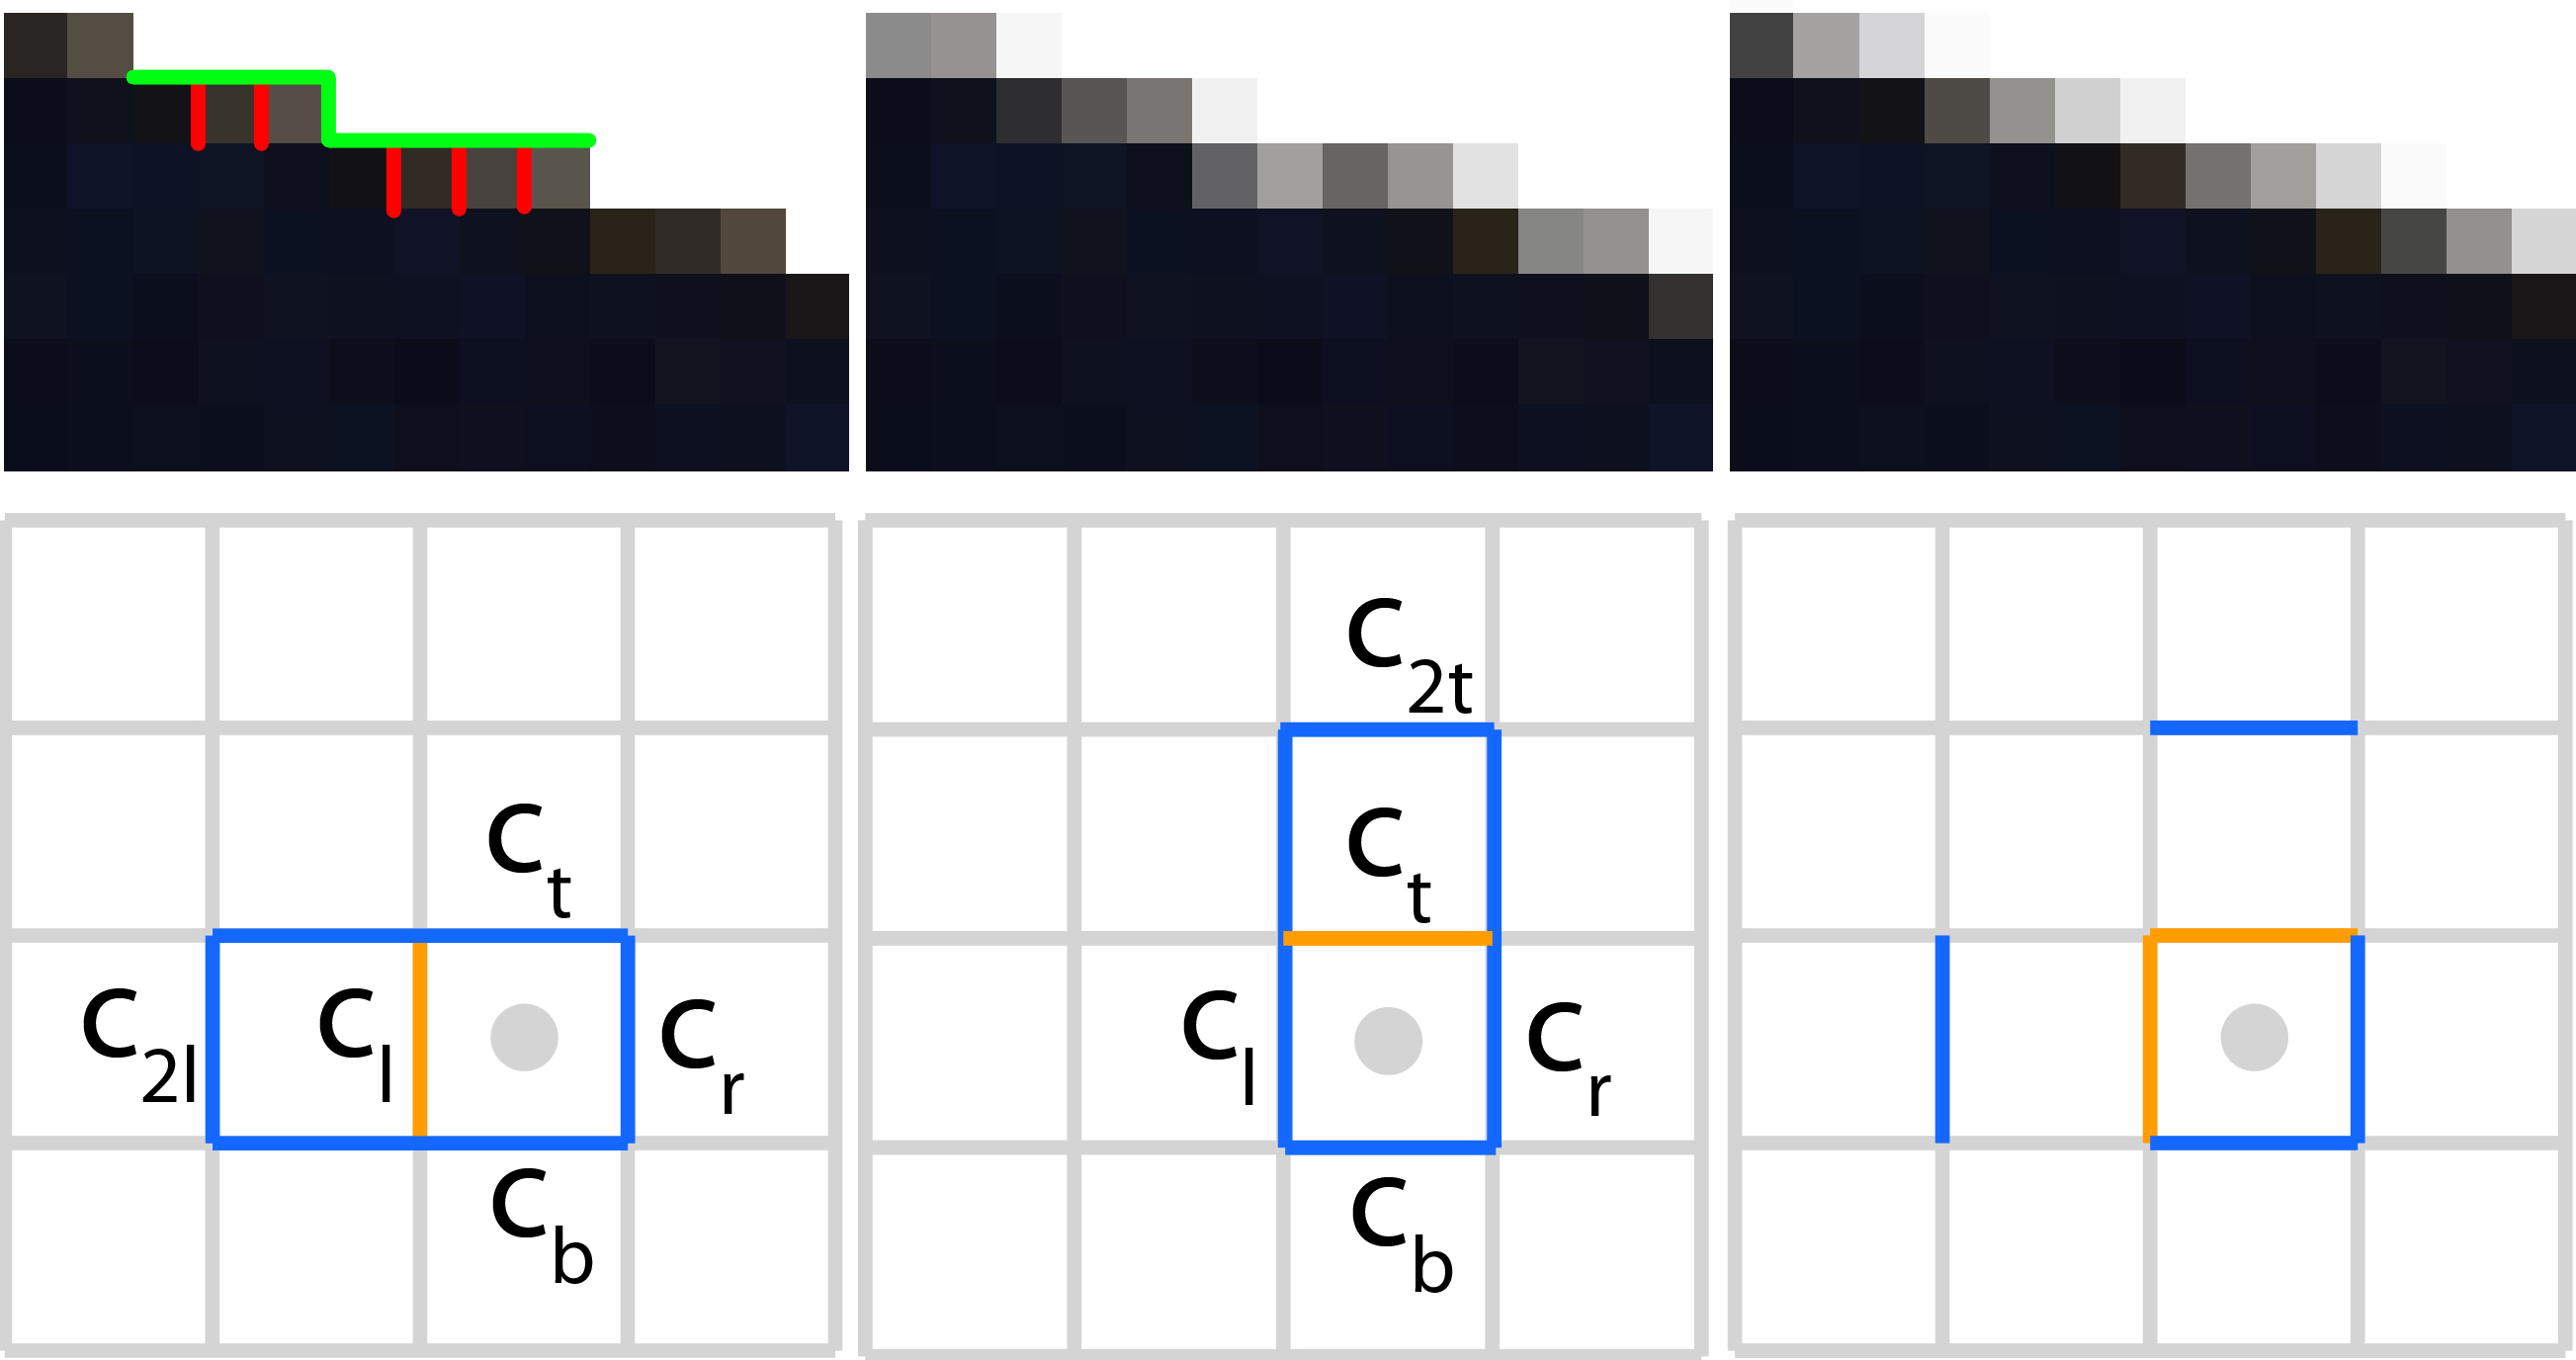
\includegraphics[width=.65\textwidth]{figures/shade/local-contrast-adaptation}
	\caption{仅对本地的像素边缘进行测试可能导致过多的边缘线段而使得结果不正确,SMAA使用一种适应性双阈值的技术,通过比较相邻像素的边缘来决定是否需要保存当前像素的边缘,这样使得较长的轮廓线上的颜色过度更平滑}
	\label{f:shade-local-contrast-adaptation}
\end{figure}

SMAA采样一种适应性双阈值(adaptive double threshold)\index{适应性双阈值adaptive double threshold}\index[en]{adaptive double threshold适应性双阈值}的策略来克服这种问题,这种策略的思路如图\ref{f:shade-local-contrast-adaptation}下左所示,其中灰色的点表示当前处理的像素点,黄色表示当前像素点可能的左边边缘,蓝色表示相邻像素的边缘。首先计算出所有蓝色边缘中亮度差值并取最大值$c_{\max}$,然后根据$c_{2l}>0.5\cdot c_{\max}$是否为true决定左边缘$c_l$是否存在。用同样的思路计算图\ref{f:shade-local-contrast-adaptation}下中的上边缘。然而实践中,由于计算所有边缘涉及大量的内存占用和读取,实际的算法仅选择一部分进行比较,如图\ref{f:shade-local-contrast-adaptation}下右所示。

最终的算法如下:首先计算出$e_l=|L-L_l|>T$,这里$e_l$表示边缘是否应该激活的枚举值,$L$和$L_l$分别为当前和相邻左边像素的亮度值,$T$为给定的阈值(通常在0.02到0.2之间),然后通过如下式决定边缘是否应该保留:

\begin{equation}
	\begin{aligned}
		c_{\max}&=\max(c_t,c_r,c_b,c_l,c_{2l})\\
		e^{'}_l&=e_l\wedge c_l>0.5\cdot c_{\max}
	\end{aligned}
\end{equation}

这里$c_t,c_r,c_b,c_l,c_{2l}$分别为如图\ref{f:shade-local-contrast-adaptation}下右对应边的亮度差值,${e}^{'}_l$表示当前像素的左边缘是否应该激活,对应的上边缘为${e}^{'}_t$。






\paragraph{计算权重值}
当边缘被标记出来后,混合权重(blending weights)\index{混合权重blending weights}\index[en]{blending weights混合权重}的计算包括三个步骤:首先找出每个像素中心距离其所在形状两端的距离,如图\ref{f:shade-mlaa}(b)以及其中的$d_{\rm left}$和$d_{\rm right}$距离;然后,需要找出该像素所在形状的交叉边缘,并连接两个交叉边缘中点构成一条轮廓线,如图\ref{f:shade-mlaa}(c);最后,根据这条轮廓线计算该像素的混合权重,如图\ref{f:shade-mlaa}(d)所示。

SMAA第一个通道输出的是一种包含边缘信息的纹理,其中纹理中每个像素的值要么为1(处于边缘),要么为0(非边缘像素),如图\ref{f:shade-smaa}(d)所示,因此求一个边缘像素到其所在边缘形状的两端交叉边缘的距离最简单的方法,就是每次向两个方向遍历,直到遇到边缘纹理中像素的值为0。

为了加速距离的计算,SMAA算法利用硬件支持的纹理过滤功能,每次遍历向前步进2个像素单位,如图\ref{f:shade-distance}所示。图中带颜色的小圆点表示边缘纹理上值为1的像素,五角星代表当前需要计算到交叉边缘距离的像素,菱形表示对边缘纹理进行采样的位置,可以看出它的步进为2个像素单位。

\begin{figure}
\sidecaption
	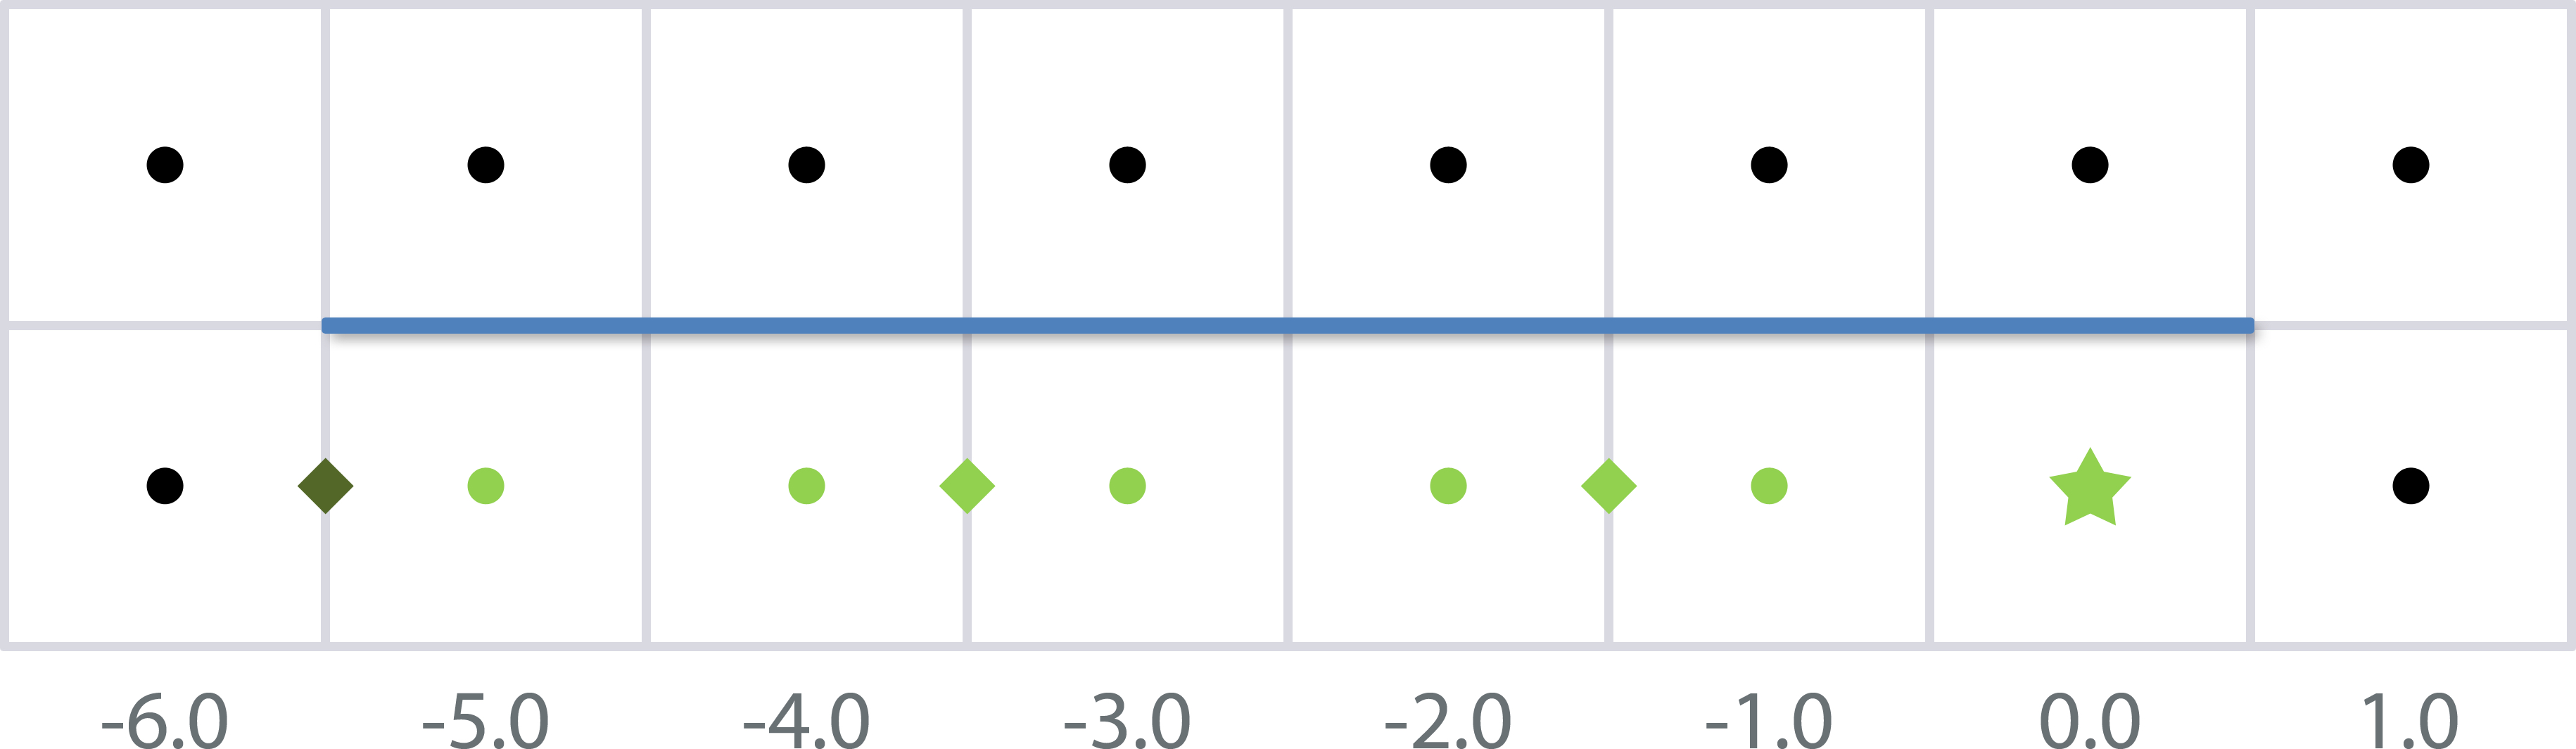
\includegraphics[width=0.65\textwidth]{figures/shade/distance}
	\caption{SMAA算法利用硬件双线性插值功能每次步进2个像素单位计算距离,它不但减少了计算量,也减少了内存读取操作以及相应的带宽占用}
	\label{f:shade-distance}
\end{figure}

由于边缘纹理上每个像素只有0和1两个值,它们均表示每个像素其中心坐标位置的值,因此从每两个相邻像素重叠的位置(菱形的地方)对边缘纹理进行采样,使用双线性插值的过滤方式将得到三种结果:

\begin{itemize}
	\item 0.0 表示两个像素均不包含边缘。
	\item 0.5 表示其中一个像素包含边缘。
	\item 1.0 表示两个像素均包含边缘。
\end{itemize}

当某次采样的值为0.5时即停止步进,它表示下一个像素不包含边缘信息,如图\ref{f:shade-distance}中的黑色的菱形位置。使用这种方法比直接对每个相邻像素进行判定要节省一半以上的计算量,同时它也减少了内存读取,节省了带宽占用。

以上是\cite{a:PracticalMorphologicalAnti-Aliasing}中采样的方法,尽管上述方法比较有效,然而却不够精确,由于它每次迭代仅在相邻两个像素的左边缘进行比较,容易忽略掉轮廓形状另一边的左边缘,例如图\ref{f:shade-accurate-distance}左下图所示,当前迭代对$b_1$和$b_2$两个像素的左边缘进行比较,但是它却忽略了$b_2$上面像素的左边缘,也就是蓝色线段,该蓝色线段本来应该导致迭代停止,因为蓝色线段就已经是交叉边缘。

\begin{figure}
	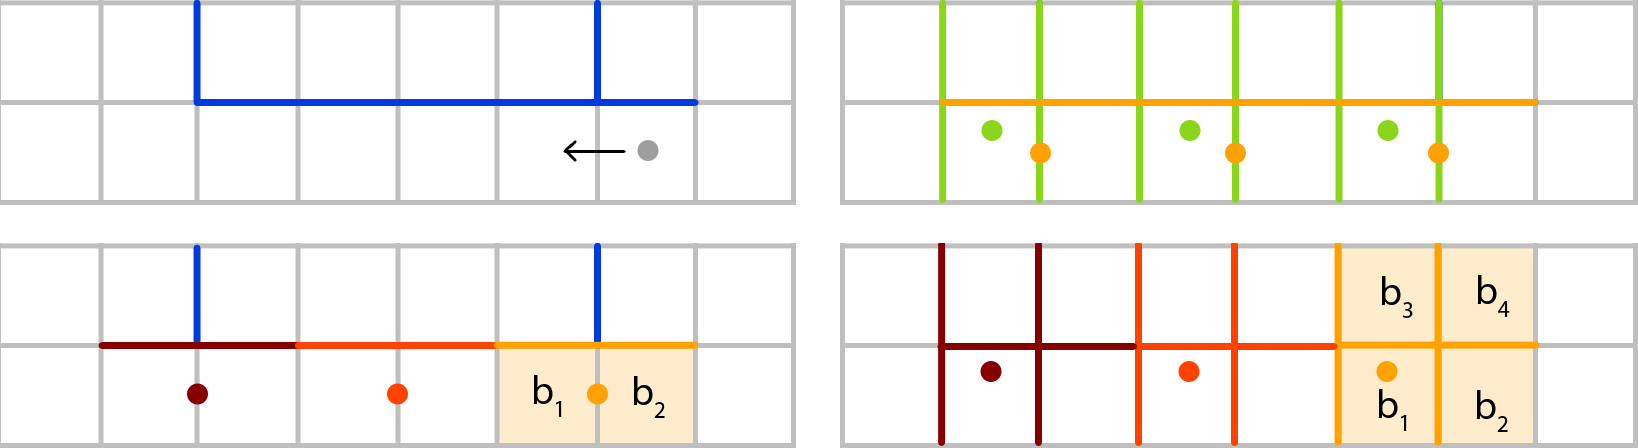
\includegraphics[width=1.\textwidth]{figures/shade/accurate-distance}
	\caption{SMAA算法使用双线性插值过滤方法,一次对4个像素进行过滤,它能够非常准确地找到交叉边缘。}
	\label{f:shade-accurate-distance}
\end{figure}

所以我们不仅需要对像素步进方向的像素左边缘进行比较,还需要对边缘形状另一边的左边缘进行判断。双线性插值本身是可以对周围的4个值进行插值的,但是由于我们将$y$轴与其中两个像素处于同一直线,导致$y$轴方向其他两个值的贡献为0,读者可以回头参照图\ref{f:intro-BilinearInterpolation}中的双线性插值方法。所以\cite{a:SMAA:EnhancedSubpixelMorphologicalAntialiasing}将采样点移到了4个边缘纹理中像素的中间部分,使得它可以取到各个点的插值,这样就可以考虑到上边像素的边缘分布,如图\ref{f:shade-accurate-distance}右下图中黄色的采样位置,它可以同时收集$b_1,b_2,b_3,b_4$的边缘信息。        

这里对纹理坐标使用了一个$(-0.25,-0.125)$的偏移,需要注意的是,edgesTex是一个RG类型的纹理,它的R用来存储每个像素的左边缘,而G用来存储上边缘,这两个分量都会被执行双线性插值采样,所以采样结果$e$是一个矢量。这里如果$e.r$为0表示$b_1,b_2,b_3,b_4$四个像素都没有左边缘,即是没有交叉边缘,所以迭代可以继续;$e.g>0.8281$用来保证$b_1,b_2$的上边缘始终存在的,否则一定应该有交叉边缘的出现。

当找到当前边缘形状两边的结束位置之后,我们还需要找到具体的交叉边缘的位置,同样使用和距离计算一样的双线性插值可以避免多次纹理读取。但是这里有一个小技巧,这里不光是需要知道哪条边是交叉边缘,为了避免条件语句的比较,这里直接将它们的返回值编码为一个特定的值,然后用这些值代表的顺序生成后面使用的面积纹理,面积纹理如图\ref{f:shade-smaa}(c)所示,我们在后面将会介绍。

\begin{figure}
	\begin{subfigure}[b]{0.24\textwidth}
		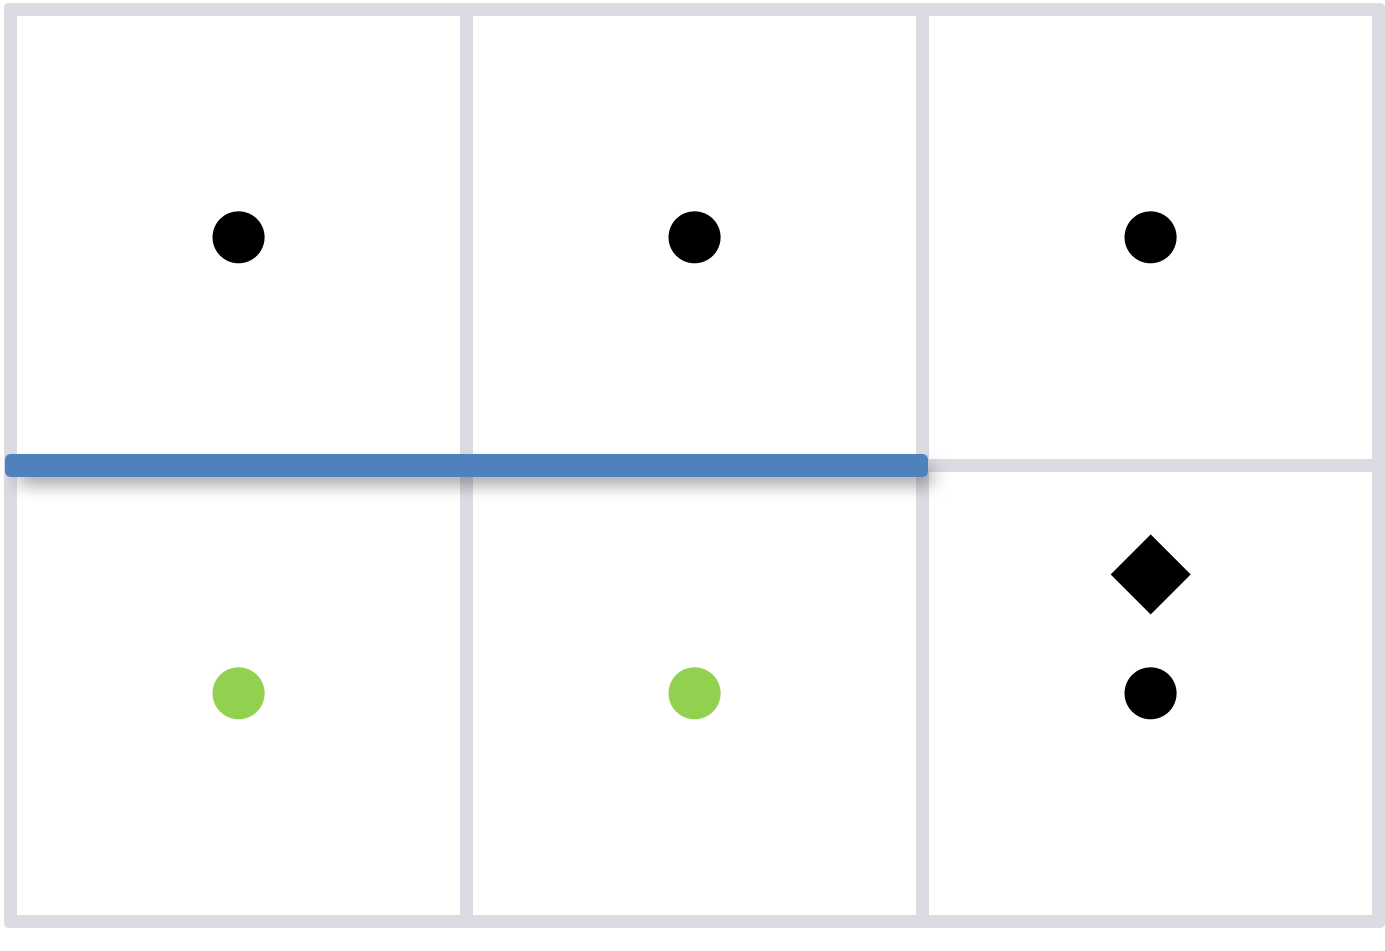
\includegraphics[width=1.\textwidth]{figures/shade/crossing-edges-1}
		\caption{0.0}
	\end{subfigure}
	\begin{subfigure}[b]{0.24\textwidth}
		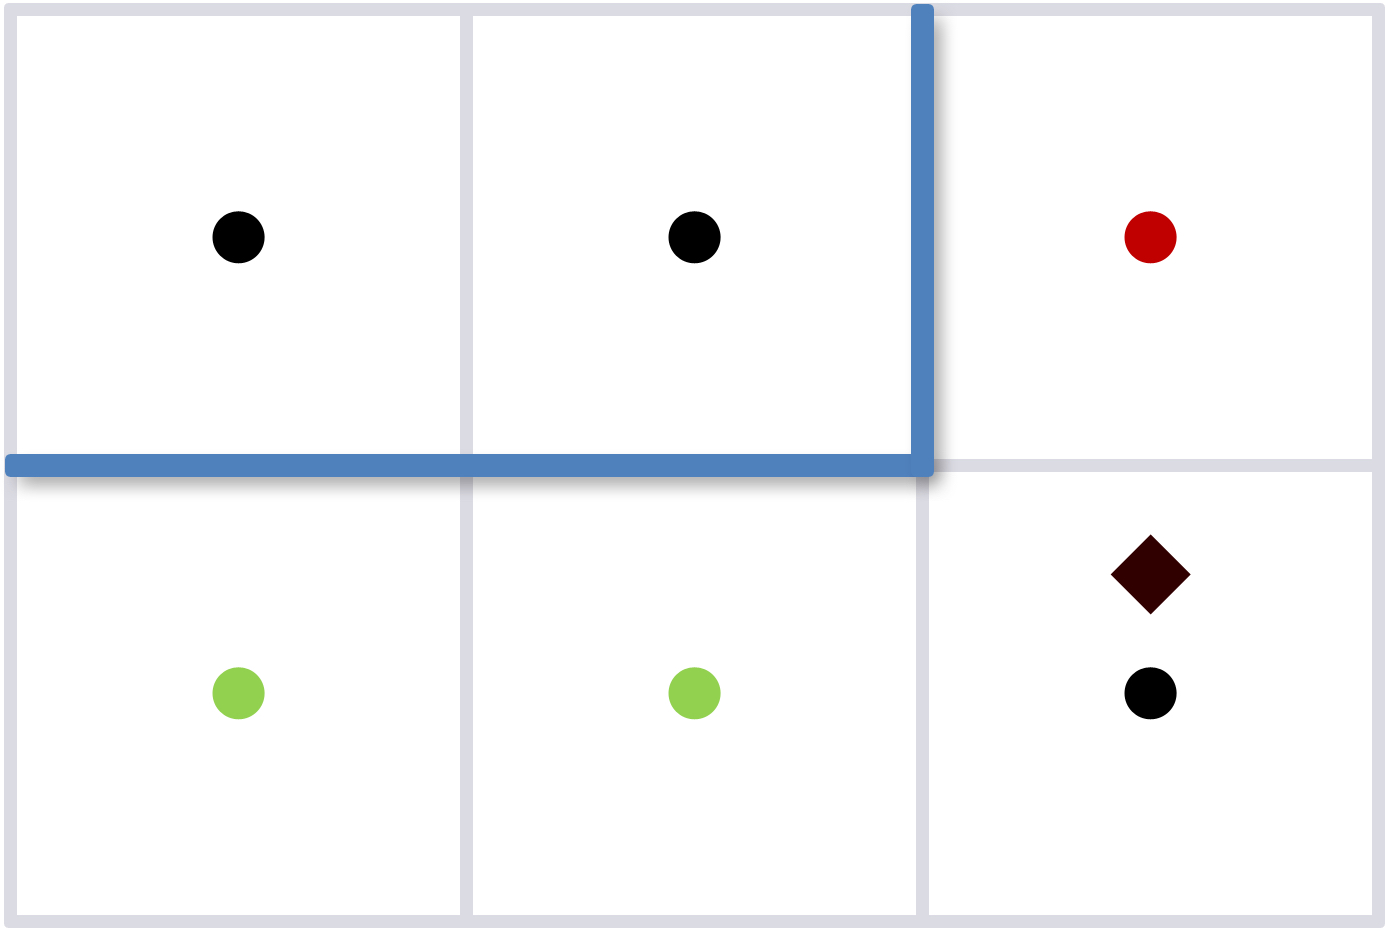
\includegraphics[width=1.\textwidth]{figures/shade/crossing-edges-2}
		\caption{0.25}
	\end{subfigure}
	\begin{subfigure}[b]{0.24\textwidth}
		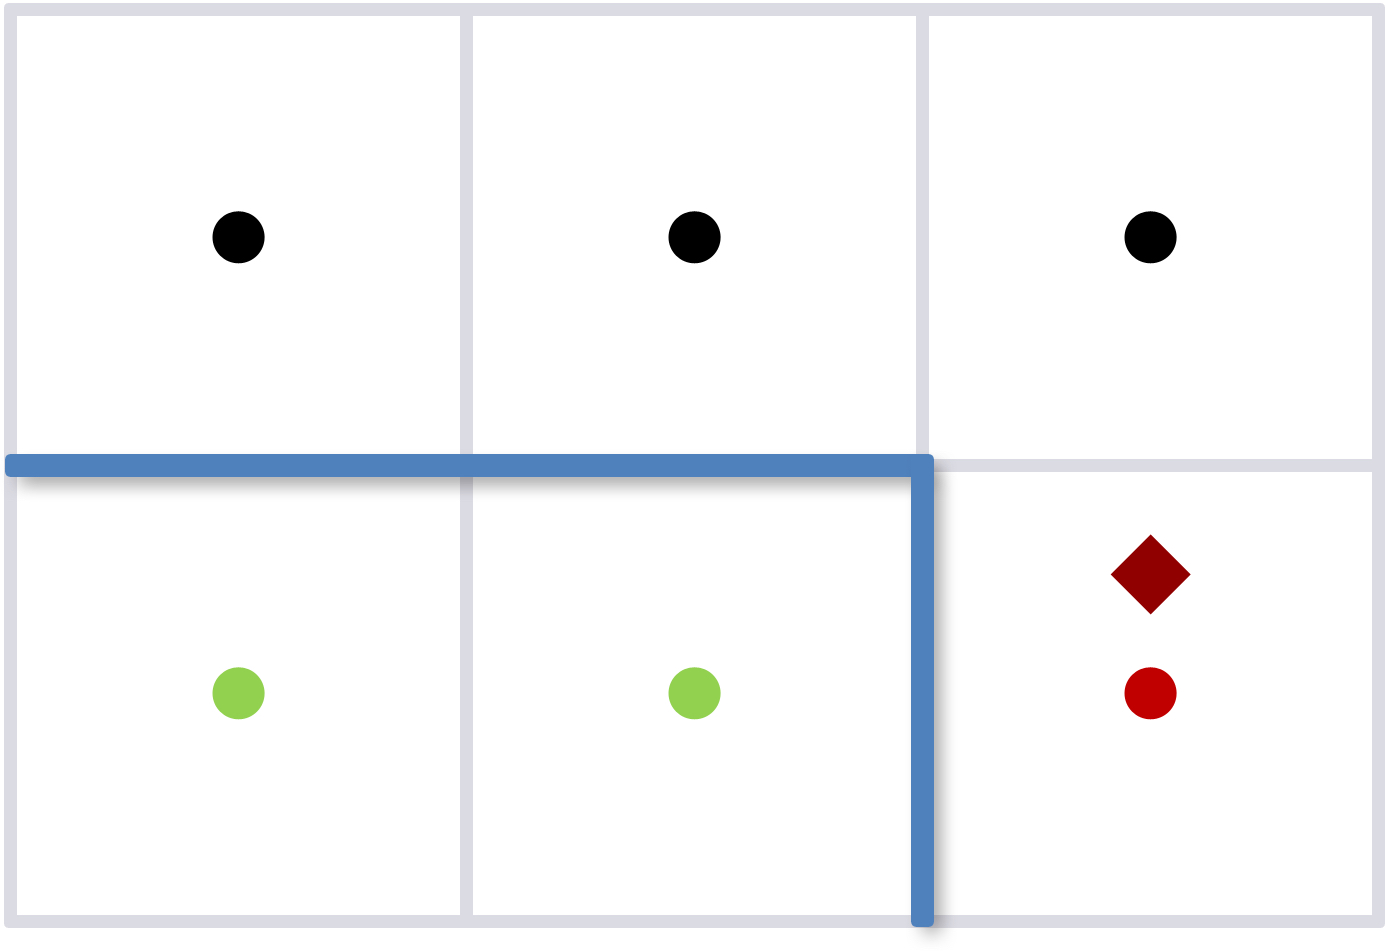
\includegraphics[width=1.\textwidth]{figures/shade/crossing-edges-3}
		\caption{0.75}
	\end{subfigure}
	\begin{subfigure}[b]{0.24\textwidth}
		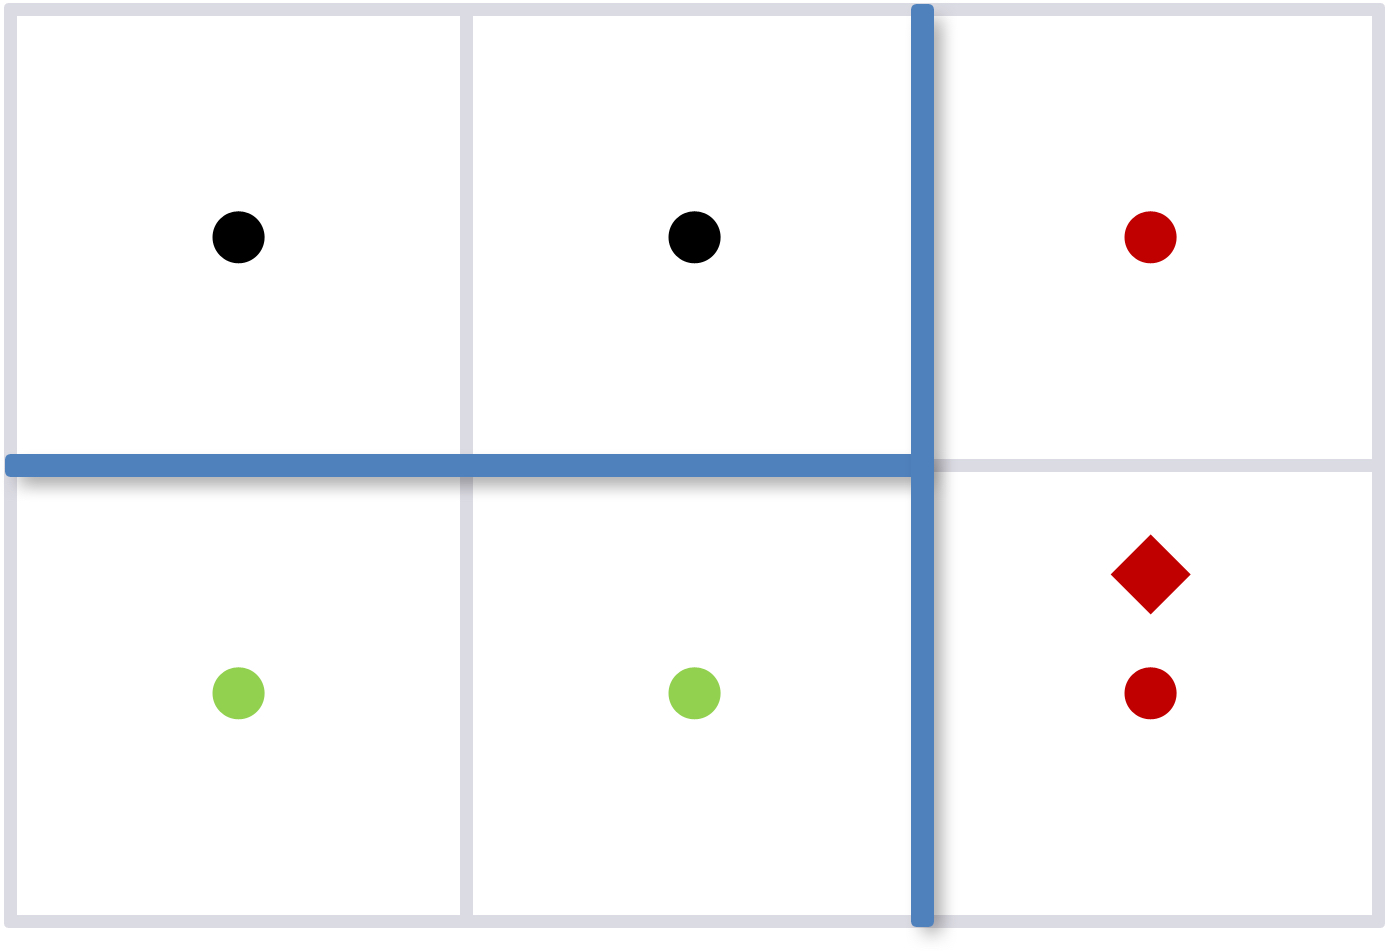
\includegraphics[width=1.\textwidth]{figures/shade/crossing-edges-4}
		\caption{1.0}
	\end{subfigure}
\caption{4种可能的右交叉边缘,使用一个(0.0,-0.25)偏移之后对边缘纹理进行采样,得到图中对应的返回结果被用于后面的面积纹理查询。}
\label{f:shade-crossing-edges}
\end{figure}

这里对像素使用一个$(0.0,-0.25)$的偏移后再对边缘纹理进行双线性插值采样,得到如图\ref{f:shade-crossing-edges}中的4个返回值,这4个值乘以4之后变成0,1,3,4四个值作为后续计算的一个索引值,避免了着色器中的条件判断。

现在我们有了每个像素到两个交叉边缘的距离,以及每个交叉边缘的类型,剩下的就是利用这些值来计算边缘像素的覆盖面积。首先我们需要将交叉边缘的中点连接起来,然后计算每个像素内梯形的面积,由于每个像素涉及大量的计算(例如还要梯形与像素交叉的点,然后进行面积计算),所以SMAA仍然将这些计算逻辑保存在一个面积纹理中。

\begin{figure}
\begin{fullwidth}
	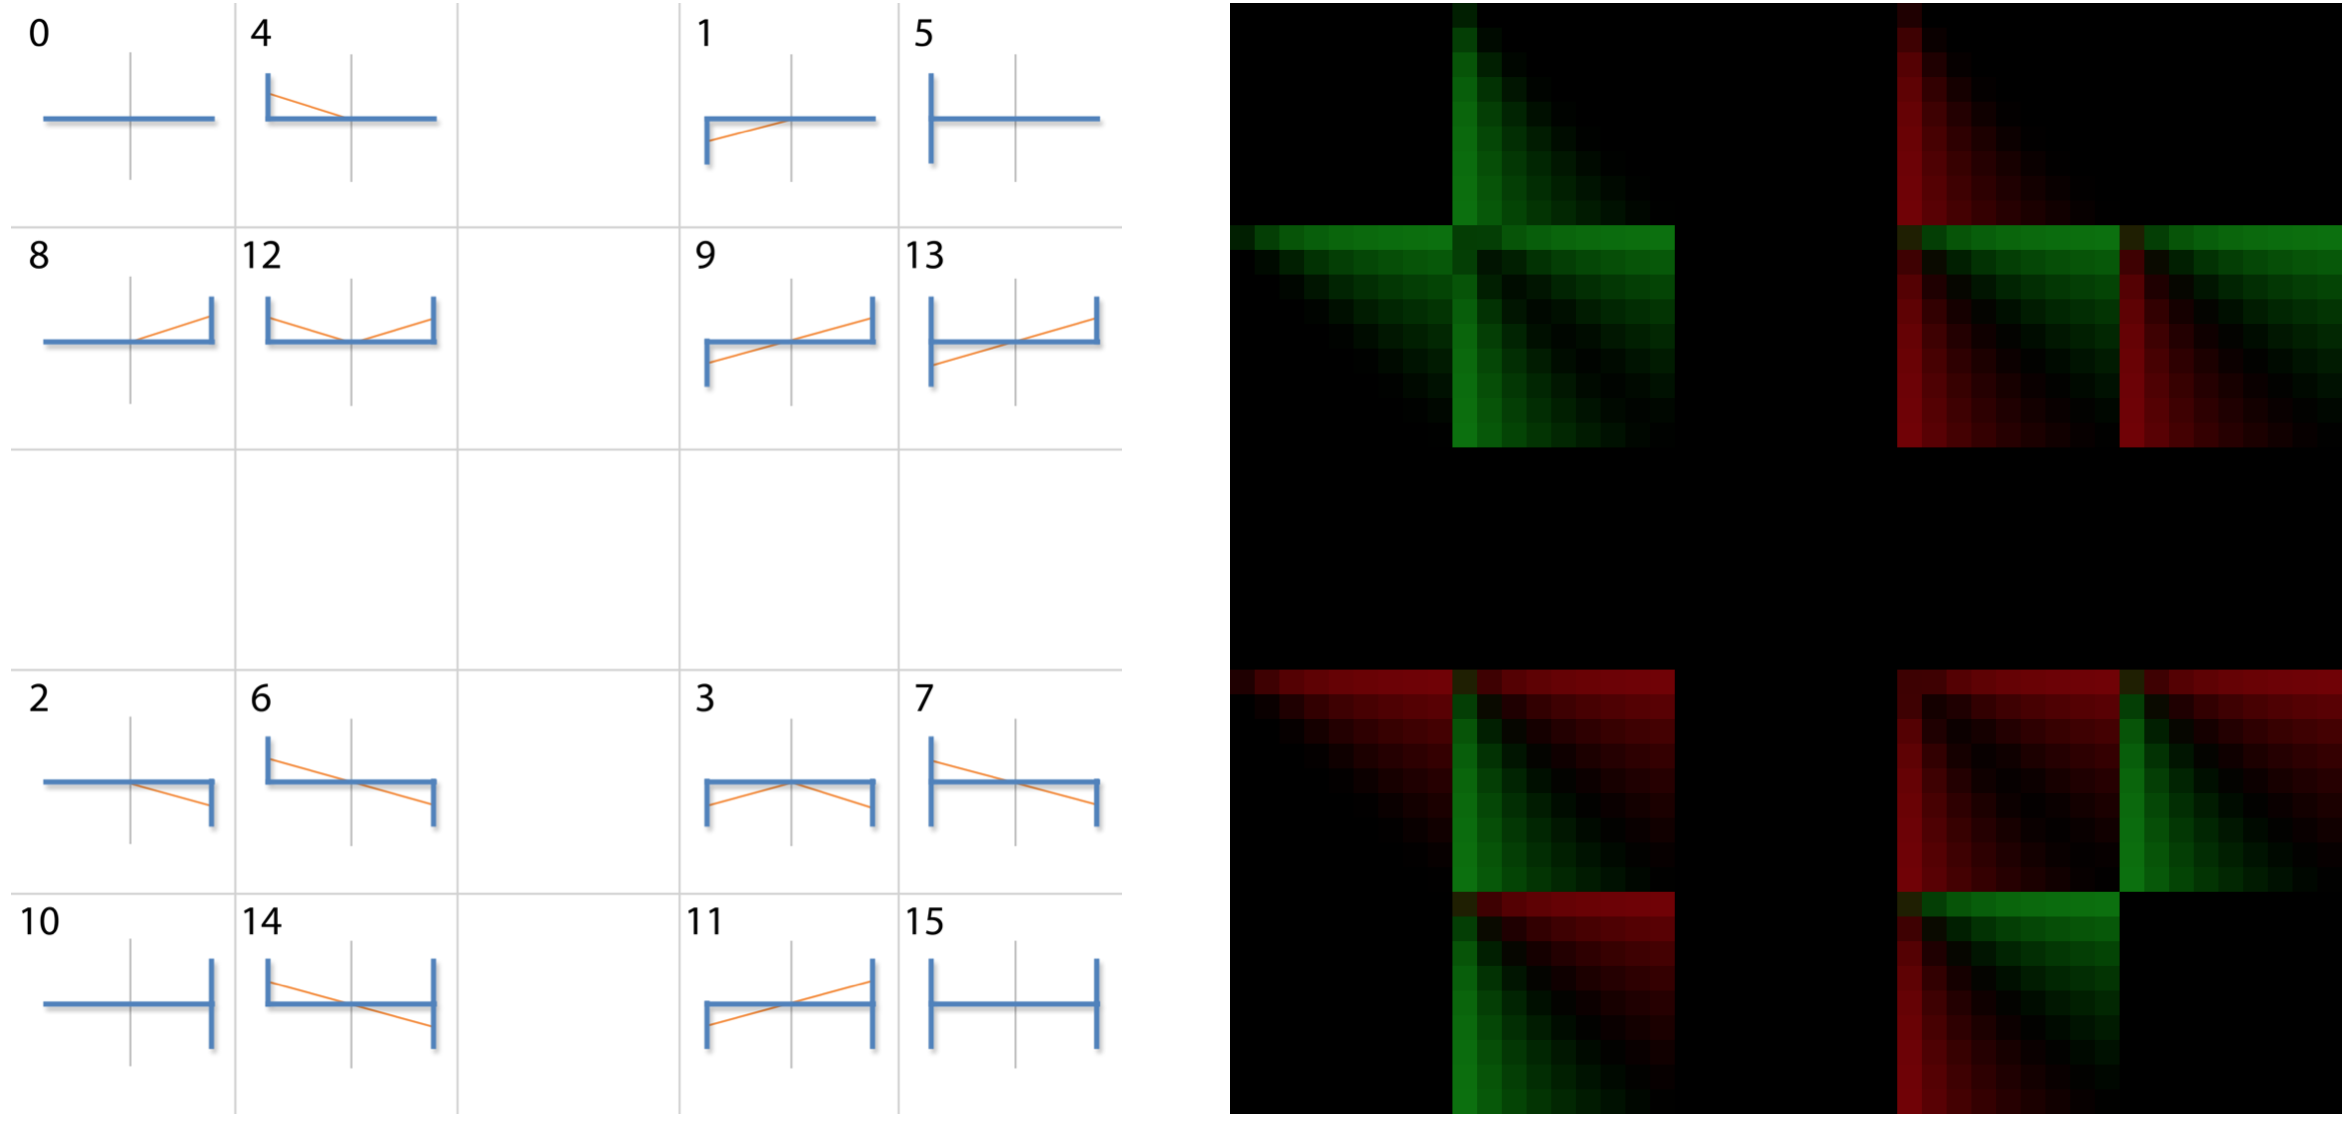
\includegraphics[width=\thewidth]{figures/shade/edge}
	\caption{面积纹理是一个多个$9\times 9$分辨率的子纹理组成,每个子纹理的坐标表示像素离两个交叉边缘的距离,这样通过预计算的面积查询,节省了着色器中复杂面积的实时计算。}
	\label{f:shade-edge}
\end{fullwidth}
\end{figure}

面积纹理(area texture)\index{面积纹理area texture}\index[en]{area texture面积纹理}是由25个$9\times 9$的子纹理(subtexture)\index{子纹理subtexture}\index[en]{subtexture子纹理}组成的纹理,如图\ref{f:shade-edge}所示,每个子纹理表示一个边缘形状类型,每个形状类型可以由2个0到4的索引值查询,这些索引值即是前面交叉边缘求得的数值,其中索引值2是不存在(思考交叉边缘的双线性插值采样的返回值不可能是0.5)。每个子像素采样的纹理坐标为每个像素距离两个交叉边缘的距离,这里的最大值9是一个优化选项,它表示前面的距离计算的迭代最大次数为9,当然也可以根据需要采样不同的值,但是必须和这里子纹理的分辨率保持一致。

Jimenez的SMAA算法是一种非常高效的反走样技术,它被用于大量的大型游戏及游戏引擎当中,其中的一些着色器编程方法和思路尤其值得学习,这也是CPU编程和GPU编程的不同的地方,其也是本节花这么多篇幅介绍的原因。SMAA\cite{a:SMAA:EnhancedSubpixelMorphologicalAntialiasing}还包括其他一些进一步的优化,以及与MSAA的整合,限于篇幅,这里将这些有趣的内容留给读者去研究。






\subsection{时间反走样}\label{sec:shade-temporal-anti-aliasing}
尽管SMAA具有非常高效的性能(这得益于它没有直接渲染子像素,以及优秀的GPU硬件优化),以及媲美$4\times$MSAA甚至以上的图像质量,但是也正是它基于单个像素进行反走样的前提,使得它不能处理子像素特征,子像素\index{子像素subpixel}\index[en]{subpixel子像素}采样对于着色走样\index{着色走样shader aliasing}\index[en]{shader aliasing着色走样}非常重要(例如超薄表面,较远的物体,高光函数,以及其他高频函数的采样),所以这使得我们又将目光转向反走样的黄金标准:超采样反走样(SSAA)\index{超采样反走样supersample anti-aliasing}\index[en]{supersample anti-aliasing超采样反走样}。

SSAA是一种空间反走样(spatial anti-aliasing)\index{空间反走样spatial anti-aliasing}\index[en]{spatial anti-aliasing空间反走样}技术,它在一个像素点的范围内,使用多个(而不是单个)采样点对场景进行渲染,然后使用一个空间过滤器(spatial filter)\index{空间过滤器spatial filter}\index[en]{spatial filter空间过滤器}将这些子像素混合成最终的单个像素。这种空间反走样技术几乎可以克服渲染过程中所有走样问题,然而每一帧渲染更多子像素的代价却非常高。

SSAA的每个子采样点通常是不重合的,因此如果我们能将这些子采样点的空间分布,分散地分布到各个时间帧中,就能实现和SSAA几乎一样的效果,如图\ref{f:shade-spatial-to-temporal}所示,这正是分期超采样\cite{a:AmortizedSupersampling}(amortized supersampling)\index{分期超采样amortized supersampling}\index[en]{amortized supersampling分期超采样}反走样的基本思路,由于这种反走样技术由空间域变换到了时间域,所以分期超采样反走样以及它后来的很多变种技术,都简称为时间反走样(temporal anti-aliasing,TAA)\index{时间反走样temporal anti-aliasing}\index[en]{temporal anti-aliasing时间反走样}。

\begin{figure}
	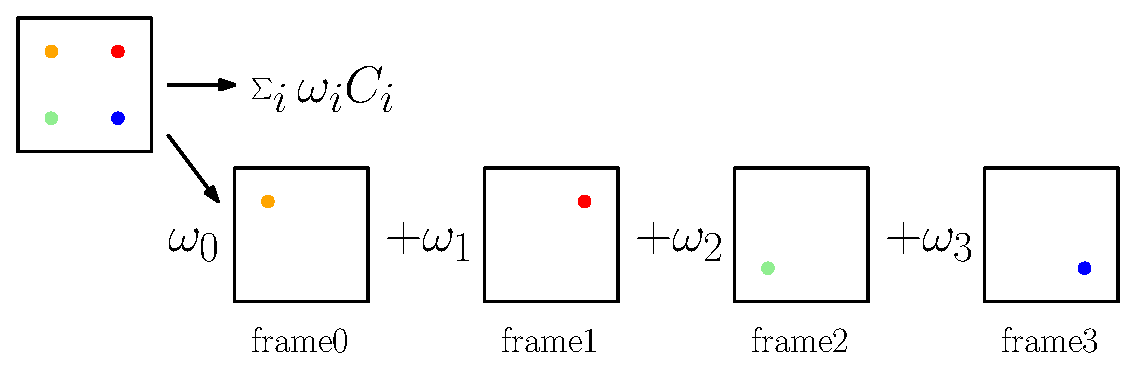
\includegraphics[width=\textwidth]{figures/shade/taa}
	\caption{分期超采样反走样技术的基本思路是将空间内个多个采样点分布到多个时间帧中,这使得它几乎呈现和超采样一样的效果。}
	\label{f:shade-spatial-to-temporal}
\end{figure}

\begin{shaded}
准确来讲,分期超采样反走样技术并不能称为时间反走样。	时间走样通常是指由于对时间域的采样不足导致的走样类型,真实的摄像机在捕捉光线的时候有一个快门时间,而计算机渲染图像不管什么时候都是某一个特定“静止”时间的静态图,因此时间采样不足就会严重丢失某些信息,例如马车轮效应(wagon-wheel effect)\index{马车轮效应wagon-wheel effect}\index[en]{wagon-wheel effect马车轮效应}。在计算机图形学中,对时间域的反走样技术通常是使用更多的时间采样(例如使用更高的帧率,或每帧渲染多个不同时刻的图像)来进行混合,在这些样本点中,变化的是时间参数。而分期超采样虽然也是分布在多个时间内,但是它本质上仍然是空间采样技术,因为它的采样参数是在空间域,它并没有对时间域进行混合。所以,本书中的TAA泛指以上这两种反走样技术,读者需要根据不同的背景内容来进行区分。
\end{shaded}






\subsubsection{静态场景}
要使用TAA技术,在不同的帧当中相同的像素应该被使用一个抖动(jittering)\index{抖动jittering}\index[en]{jittering抖动}操作,以使当前帧的像素被移动到一个超采样中子采样点的位置。抖动的位移通常使用某种随机分布函数(第\ref{chp:mc}章介绍)产生,由于这些子采样点全部会被混合起来,所以为了达到更好的图像质量,该随机分布应该具有低差异性(low discrepancy)\index{低差异性low discrepancy}\index[en]{low discrepancy低差异性},子采样点的分布尽量铺满整个像素区域,在Unreal Engine 4和神秘海域4中他们均使用Halton数列\footnote{参见:\url{http://en.wikipedia.org/wiki/Halton_sequence}}(Halton sequence)\index[en]{Halton sequenceHalton数列}来产生子采样点的分布,如图\ref{f:shade-halton}所示。

\begin{figure}
	\sidecaption
	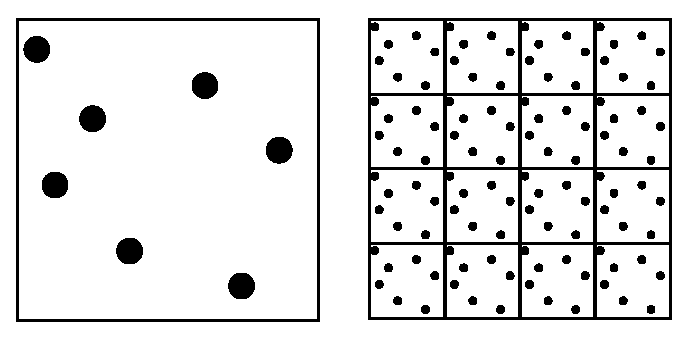
\includegraphics[width=0.5\textwidth]{figures/shade/halton}
	\caption{Halton数列}
	\label{f:shade-halton}
\end{figure}

为了不影响渲染管线的结构及流程,这个像素的抖动操作通常发生在顶点着色器中,通过直接修改投影矩阵,将原本正常的位于像素点中心的采样点修正到偏移位置,这里可以通过如下的代码来对投影矩阵进行修改:

\begin{lstlisting}[language=C++]
ProjMatrix[2][0] += ( SampleX * 2.0f – 1.0f ) / ViewRect.Width();
ProjMatrix[2][1] += ( SampleY * 2.0f – 1.0f ) / ViewRect.Height();
\end{lstlisting}

通过抖动,产生了和SSAA一样的空间域上的多个子采样点。接下来,和SSAA一样,我们还需要一个空间过滤器来对这些子采样点进行过滤,最简单的方式是使用一个盒子过滤器,它对像素内所有的子采样点求加权平均值,其形式如下:

\begin{equation}
	s_t=\frac{1}{n}\sum^{n-1}_{k=0}x_{t-k}
\end{equation}

其中,$s_t$表示第$t$时间帧的最终混合结果,$x_t$为第$t$时间帧单帧的绘制结果,它被用于显示在屏幕上。这种混合方式虽然简单,然而它要求帧缓存存储$n$个时间帧的绘制结果,这无疑会耗费巨大的内存,\cite{a:PixelCorrectShadowMapswithTemporalReprojectionandShadowTestConfidence,a:AcceleratingReal-TimeShadingwithReverseReprojectionCaching}使用了一种递归指数过滤器(recursive exponential filter),它直接使用当前渲染的结果$x_t$和之前所有帧混合的经过反走样处理的历史结果$s_{t-1}$进行混合,即:

\begin{equation}\label{eq:shade-exponential-filter}
	s_t=\alpha x_t+(1-\alpha)s_{t-1}
\end{equation}

由于这种方法非常高效,因此它被当前主流游戏引擎大量使用。这里的混合系数$\alpha$决定着图像由走样到平滑过渡的快慢:较小的$\alpha$意味着每一帧在总的最终图像中的贡献越小,而最终图像则可以由更多采样点的混合决定,因此最终图像质量更高,但是它的逼近过程却很慢;反之$\alpha$越大,逼近过程越快,但是由于当前走样的渲染结果占据太大的比重,因此最终图像质量相对较低。神秘海域4\cite{a:TemporalAntialiasingInUncharted4}中选择的混合系数为0.05,其TAA通道中的结果计算方式如下\footnote{注意,对于静态场景直接使用Load函数,它不对纹理执行任何过滤操作,由于静态场景中每个物体的坐标是完全不变的,因此这里直接读取精确的结果,这不同于后面动态场景使用的Sampe方法,它需要对历史结果进行过滤因此带来模糊,所以静态场景理论上可以对每个像素使用无穷多个不同偏移的子采样点而带来更精确的结果。}:

\begin{lstlisting}[language=C++]
float3 currColor = currBuffer.Load(pos);
float3 historyColor = historyBuffer.Load(pos);
return lerp(historyColor, currColor, 0.05f);
\end{lstlisting}

\cite{a:HighQualityTemporalSupersampling}说明当$\alpha$很小时,指数逼近的结果和加权平均的结果是一致的,即:

\begin{equation}
\begin{aligned}
	s_t=\alpha x_t+(1-\alpha)s_{t-1}=\alpha &\sum^{\infty}_{k=0}(1-\alpha)^{k}x_{x-t}\\
	x_t=x_{t-n}\Rightarrow s_t=\frac{\alpha}{1-(1-\alpha)^{n}}&\sum^{n-1}_{k=0}(1-\alpha)^{k}x_{t-k}\\
	\lim_{\alpha\rightarrow 0}\frac{\alpha}{1-(1-\alpha)^{n}}&\sum^{n-1}_{k=0}(1-\alpha)^{k}x_{t-k}=\frac{1}{n}\sum^{n-1}_{k=0}x_{t-k}
\end{aligned}
\end{equation}

那么TAA的混合计算应该在延迟渲染中的哪个阶段执行呢?在神秘海域4中他们在延迟着色计算之后,对高动态范围(high dynamic range,HDR)\index{高动态范围high dynamic range}\index[en]{high dynamic range高动态范围}的图像进行时间反走样处理,然后将时间反走样之后的HDR图像传给渲染管线的后续阶段,例如色调映射(tone mapping)\index{色调映射tone mapping}\index[en]{tone mapping色调映射}及其他后处理阶段。







\subsubsection{动态场景}
当场景是动态的时:例如物体移动,摄像机移动,光源移动或变化导致遮挡关系发生变化,还有大量(在着色器中)通过程序控制的几何体(如海面,头发等),这时TAA的处理开始变得复杂。对于TAA,理想状态下,我们需要的是除了采样点位置外完全一致的两个像素点,然而当像素被移动时,这一切都可能发生变化。

我们首先来概述一下动态场景带来三个最重要的问题,让读者首先有个思路,然后再分述每个问题的解决方案。基本来讲,动态场景带来以下三个新的问题:

\begin{itemize}
	\item 首先,需要一个额外的屏幕区域大小的缓存来存储每个历史颜色的位置,这通过在延迟着色的G-buffer阶段通过将当前像素位置重投影到上一帧中摄像机的变换矩阵来计算,计算结果存储在G-buffer中供TAA使用。
	\item 由于重投影的操作,我们需要在上一帧图像的离散的屏幕分辨率中找出一个位置来对历史颜色缓存进行采样,这涉及重采样(resampling)\index{重采样resampling}\index[en]{resampling重采样}的问题,因此可能使结果变得模糊。
	\item 由于场景发生变化,同一位置的像素除了采样点位置外可能发生了其他变化:例如光源遮挡关系,像素颜色值发生变化,甚至像素本身是由着色器中程序产生的几何体,它一直都在变化,这样的变化将可能导致重影的瑕疵。
\end{itemize}

以下我们详述每个问题的原因,解决思路以及解决方法的细节,其中有些问题可能有多种解决方案。







\paragraph{重投影}
TAA需要获取历史颜色值,因此当场景发生移动时,我们需要找出当前帧中每一个像素在上一帧当中的位置,如图\ref{f:shade-reprojection}所示,这通过称为重投影(reprojection)\index{重投影reprojection}\index[en]{reprojection重投影}的技术的实现。

\begin{shaded*}
	重投影的概念比较早出现于\cite{a:AcceleratingReal-TimeShadingwithReverseReprojectionCaching,a:PixelCorrectShadowMapswithTemporalReprojectionandShadowTestConfidence}中,但是他们不是被用于反走样计算,相反,他们发现这样一个事实:即场景中相邻两帧中大部分像素的颜色值都是连贯的(coherence)\index{连贯的coherence}\index[en]{coherence连贯的},因此如果能够持续跟踪这些没有发生太多变化的像素,并将它们缓存起来,则下一帧可以不用再重新计算该像素的颜色,因此他们要实现的实际上是一个缓存系统。
	
	但是这两者的思路是一致的,即都是通过找出当前帧像素在历史颜色缓存中的位置,然后对历史颜色缓存进行采样,只是采样后的值的用途不一致。所以,这两者可以实现相同的技术,也因此它们拥有相同的由于重采样导致的模糊问题,但是被用作缓存目的并不会有后面讨论的重影现象。关于像素的连贯性还会被本书后面的其他一些全局光照算法使用。
\end{shaded*}

\begin{figure}
	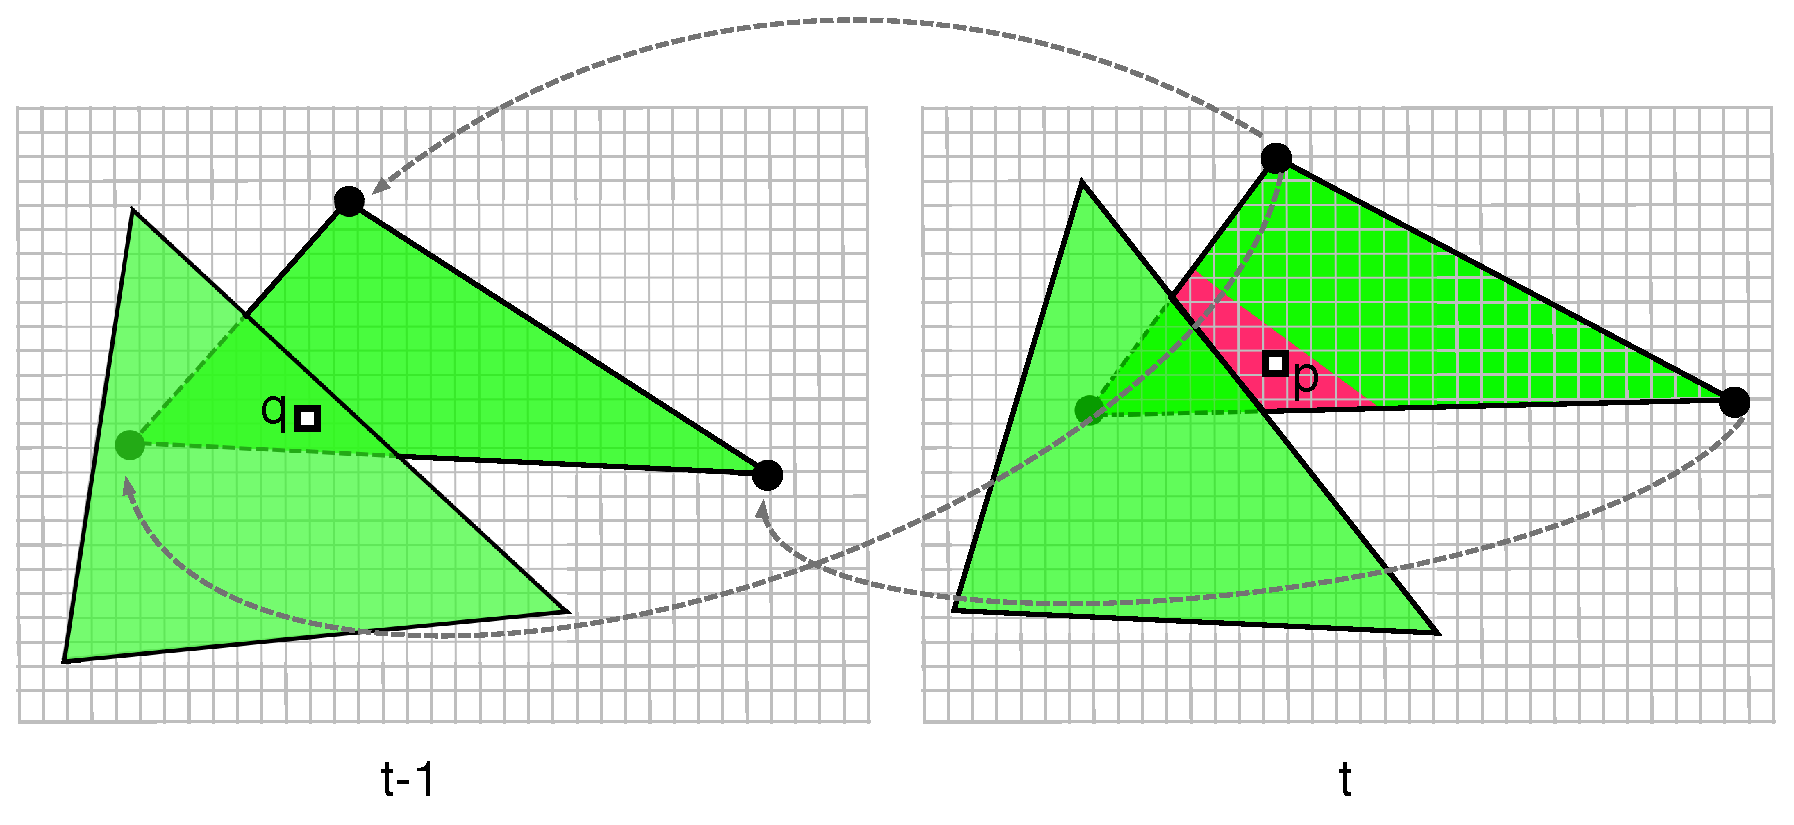
\includegraphics[width=\textwidth]{figures/shade/reprojection}
	\caption{TAA需要知道当前帧每个像素在历史颜色缓存中的位置,这需要对每个像素计算一个移动矢量,然后在TAA中用来对历史颜色采样,注意由于发生移动,场景中同一位置的像素颜色,深度,遮挡关系等可能发生变化,例如第t帧的p点对应第t-1帧的q点由不可见变为可见。}
	\label{f:shade-reprojection}
\end{figure}

为了计算当前像素在历史颜色缓存中的位置,通常在延迟着色的几何通道中同时计算出每个像素在上一帧相对于当前帧的偏移位置,这称为一个移动矢量(motion vector)\index{移动矢量motion vector}\index[en]{motion vector移动矢量},然后使用一个额外的颜色缓存将偏移矢量直接输出到G-buffer中,为了保证精度,通常使用RG16格式。这需要在几何通道中输入以下数据:上一帧的摄像机信息以及上一帧每个物体的本地到世界坐标的变化矩阵$mat_{o2w}$,然后在顶点着色器中同时输出相邻两帧的顶点坐标到片元着色器中,即:

\begin{lstlisting}[mathescape=true]
$pos_{proj}$ = $pos_{obj}$ x $mat_{wvp}$
$posLast_{proj}$ = $posLast_{obj}$ x $matLast_{wvp}$
\end{lstlisting}

这些顶点坐标被光栅化处理后,就可以在片元着色器中计算每个像素的移动矢量,并输出到G-buffer中供TAA使用:

\begin{lstlisting}[mathescape=true]
$pos_{ndc}$ -= g_projOffset;
$posLast_{ndc}$ -= g_projOffsetLast;
float2 motionVector=($posLast_{ndc}$-$pos_{ndc}$)* float2(0.5f, -0.5f);
\end{lstlisting}

需要注意的是,这里需要使用去除抖动的坐标(上一帧的抖动值包含在摄像机信息中),因为对于历史颜色缓存而言,它存储的是每个像素中心点位置的颜色值,哪些抖动的子像素位置仅是用来进行不同的采样,然后这些子采样点被按照像素中心点的位置进行过滤,如果我们直接使用抖动过的位置,则计算出的结果可能是两个完全不同的像素位置;另一点需要注意的是,由于在后面的TAA阶段需要通过纹理坐标(即[0,1]的范围)来对历史颜色缓存(一个2D纹理)进行采样,所以我们需要在NDC空间计算移动矢量。

有了移动矢量缓存,在TAA中就可以直接对当前对历史颜色缓存进行采样,即:

\begin{lstlisting}[language=C++]
float2 uvLast = uv + motionVectorBuffer.Sample(point, uv);
float3 historyColor = historyBuffer.Sample(linear, uvLast);
\end{lstlisting}

然而,与静态图像不一样的是,由于光栅化计算出的像素坐标仅仅是一个像素的中点,所以当摄像机或物体发生移动时,同样的点光栅化之后的坐标并不是完全一样的,它可能存在小于一个像素内的偏移,有时候甚至被定位到了不相关的位置\cite{a:TemporalAntialiasingInUncharted4}。所以,对于历史颜色缓存的采样不能直接使用Load函数,而需要对其使用Sample函数进行过滤,而这种过滤导致了最终颜色变得模糊,尤其当历史颜色缓存累积的越多,它越被使用了更大范围的像素进行过滤。因此模糊处理成为TAA的一个需要处理的重要问题。







\paragraph{模糊处理}
TAA中的模糊来源于在每次迭代中,对历史颜色纹理的采样使用了双线性过滤器,这样历史颜色的采样值来源于该像素周围4个像素颜色值按一定的权重比例的加权和(weighted sum)\index{加权和weighted sum}\index[en]{weighted sum加权和},而这些周围参与加权的像素的颜色来源于更早历史周围的加权和,以此类推,随着时间的增加,参与加权的像素的范围就越来越大。

为了理解TAA中的模糊的原因,以及寻找解决方案,\cite{a:AmortizedSupersampling}用公式表示出了这种重投影的方差:

\begin{equation}
	\sigma^{2}_v=\sigma^{2}_G+\frac{1-\alpha}{\alpha}\frac{v_x (1-v_x)+v_y(1-v_y)}{2}
\end{equation}

式中$\sigma^{2}_G$是一个常数项,它表示产生抖动的随机数的方差,$v$表示像素中心距离每个子采样点的差值(如图\ref{f:shade-blur-factor-filter}所示)。由该式可以看出,影响重投影模糊的有两个因素,它分别对应两种消除模糊的方案。第一是减少每个子采样点到像素中心点的距离$v$,如图\ref{f:shade-blur-factor-filter}所示,$v$越大,则总的过滤过程向外扩散的范围越大。针对此,比较有效的解决方法是提高分辨率,例如\cite{a:AmortizedSupersampling}就提供了一种方法,它将每个像素划分为4个子像素,但是不需要每一帧渲染4次,而是将在四个子像素独立存储为一个缓存对象,每一帧只更新一个子像素,然后将它们合并。

\begin{figure}
	\sidecaption
	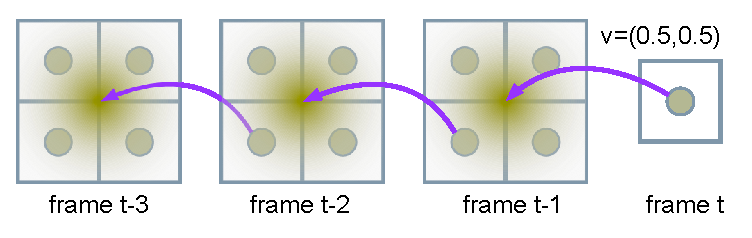
\includegraphics[width=0.65\textwidth]{figures/shade/blur-factor-filter}
	\caption{TAA对历史颜色缓存进行双线性过滤采样时,周围每个像素距离像素中心点的距离越大,在多次迭代中参与贡献的像素的范围就越大,图像就越模糊。}
	\label{f:shade-blur-factor-filter}
\end{figure}

另一个影响因素是混合因子$\alpha$,如图\ref{f:shade-blur-factor-alpha}所示,$\alpha$越大,则历史颜色的权重越低,所有历史像素对模糊的贡献就越小,所以算法应该选择比较合适的混合因子。

\begin{figure}
	\sidecaption
	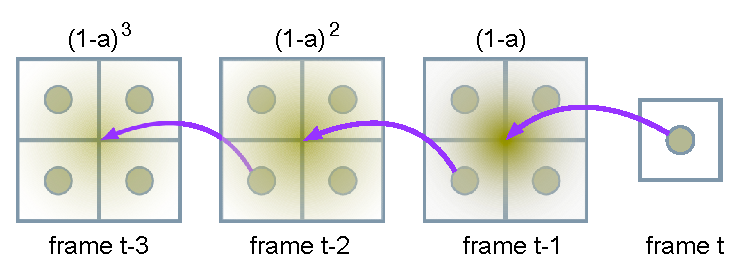
\includegraphics[width=0.65\textwidth]{figures/shade/blur-factor-alpha}
	\caption{TAA对历史颜色缓存进行双线性过滤采样时,混合因子$\alpha$越大,则历史每个颜色对总的图像的恭喜越小,因此图像越清晰。}
	\label{f:shade-blur-factor-alpha}
\end{figure}

在Unreal Engine 4中,它们使用了两种方法来控制$\alpha$以减少模糊。首先是当像素附近的颜色对比度比较低时增加混合因子,而对比度高时(例如薄面,边缘等频率变化比较高的区域)减少混合因子。在TAA中,混合因子$\alpha$并不要求总是一个常数,它可以针对不同的像素以及不同的时间帧使用不同的混合因子。

其次,为了进一步减小模糊,可以使用一个单独的通道以后处理的方式对颜色缓存进行锐化处理,这通过对颜色缓存使用一个锐化过滤器(sharpen filter)\index{锐化过滤器sharpen filter}\index[en]{sharpen filter锐化过滤器}来实现,例如神秘海域4使用以下过滤器来对周围$3\times 3$的像素区域进行混合:

\begin{equation}
\begin{bmatrix}
	0  & -1 & 0\\
	-1 & 4  & -1\\
	0  & -1 & 0
\end{bmatrix}
\end{equation}

它将对每个像素执行类似如下的计算:

\begin{lstlisting}[language=C++]
return saturate(center + 4 * center - up - down - left - right);
\end{lstlisting}

这里saturate是一个限制函数,它将执行过滤的结果限制在$[0.0,1.0]$的范围,因为锐化过滤器的加权和并不为1。





\paragraph{重~~影}
TAA最著名的问题是关于重影(ghosting)\index{重影ghosting}\index[en]{ghosting重影}的问题,它使得历史颜色值出现在了物体运动的路径中,如图\ref{f:shade-ghosting}所示。

\begin{figure}
\begin{fullwidth}
	\begin{subfigure}[b]{0.36\thewidth}
		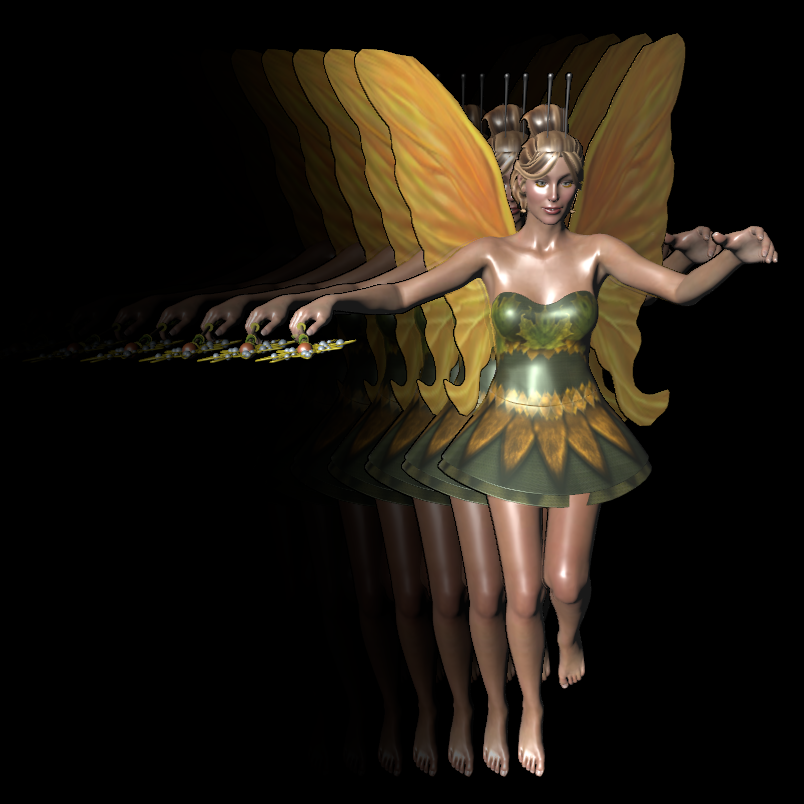
\includegraphics[width=1.\textwidth]{figures/shade/ghosting-1}
		\caption{像素级别的颜色变化}
	\end{subfigure}
	\begin{subfigure}[b]{0.628\thewidth}
		\includegraphics[width=1.\textwidth]{figures/shade/ghosting-2}
		\caption{子像素级别的颜色变化}
	\end{subfigure}
	\caption{像素颜色的变化导致历史上不在“合法”的颜色值被混合进当前颜色值,呈现出重影的效果,由于随着时间推移,历史颜色值的权重逐渐降低,因此这种重影表现为一种拖尾效果(图(a)来自Nvidia,图(b)来自顽皮狗工作室)}
	\label{f:shade-ghosting}
\end{fullwidth}
\end{figure}

根据公式\ref{eq:shade-exponential-filter},我们可以推断出现重影的原因主要是由于像素的颜色值发生了改变,但是历史不再“合法”的颜色还是被混合进了当前帧的输出图像中,随着时间的推移,历史颜色值的权重不断下降,历史颜色值逐渐变淡直至几乎肉眼无法察觉,这就形成一个拖尾的效应。

这种改变的原因大概可以分为两类:第一类是整个像素的值发生了变化,例如由原来的可见变为不可见,这个时候历史上可见的颜色值就会被混合进不可见的区域,形成比较强烈的重影,如图\ref{f:shade-ghosting}(a)所示;第二类是一个像素内的局部颜色发生了改变,即某些子采样点的颜色发生了变化,这通常发生于子像素特性中,一些地方在一个像素尺寸内的频率域变化很大(例如一些超薄表面,草地等),使得某些子像素特性无法被渲染而被历史颜色所混合,这种重影即使在第一类重影被适当处理的情况下任然会发生,例如图\ref{f:shade-ghosting}(b)就是第一类重影被处理,但是崎岖不平的路面中具有频率变化范围较大的法线的范围,仍然被人物头像部分的历史颜色所混合。

重影是由于历史颜色缓存不合法导致的混合结果,例如像素的可见性,颜色,几何体ID等发生变化都会导致历史颜色缓存中的颜色失效,对于这类失效的历史颜色,它们不应该再被混合进当前颜色中。所以,为了排除失效的历史颜色,TAA需要在混合时前判断历史颜色是否失效,这同SMAA中的边缘检测类似,可以使用多种像素的属性来进行比较,但是TAA中一般选择RGB颜色值进行比较。

目前工业中\cite{a:AnExcursioninTemporalSupersampling,a:RealtimeglobalilluminationandreflectionsinDust514,a:TemporalAntialiasingInUncharted4,a:TemporalReprojectionAnti-AliasinginINSIDE}比较流行的是称为邻域裁剪(neighborhood clamping)的方案,这种方案基于这样一个假设:即图像中的颜色是连续的,历史颜色缓存中的颜色应该位于当前时间帧内邻域像素颜色的范围内。为此,工业中这些方案中最普遍的方法是使用一个AABB包围盒在颜色空间内将当前像素的周围$3\times 3$个像素的颜色包围住,这个AABB包围盒形成了一个颜色范围,然后判断对历史颜色缓存的采样是否落在了这个颜色范围内,如图\ref{f:shade-clamping}所示。

\begin{figure}
\sidecaption
	\includegraphics[width=0.65\textwidth]{figures/shade/color-space}
	\caption{颜色空间是一个2D的平面区域,它通常由一个三角形构成,三角形的每个边表示每种颜色空间的RGB三种原色选择,在每个颜色空间内,每个颜色到三个顶点的原色的比例之和为1,不同的颜色空间能够表示的颜色数量不一样,它们之间可以相互转化,但可能存在损失(图片来自Wikipedia)。}
	\label{f:shade-clamping}
\end{figure}

为了进一步理解邻域裁剪,我们首先需要了解颜色空间的概念。颜色空间\footnote{\url{参见:https://en.wikipedia.org/wiki/Color_space}}(color space)\index{颜色空间color space}\index[en]{color space颜色空间}是一个色度学(colorimetry)\index{色度学colorimetry}\index[en]{colorimetry色度学}中的概念,在色度学中,一个颜色只由RGB三个原色混合而成的,这三个原色的混合比例的和为1,由于这个限制,所以3D空间的颜色可以表述为2D空间的颜色范围,这个范围在2D的颜色空间上表现为一个三角形,在每个颜色空间内,每个颜色值到三角形每个顶点的比例之后为1,如图\ref{f:shade-conservative-rasterization}所示,不同的RGB三原色选择导致了不同的颜色空间,从而在整个颜色域也具有不同的颜色范围。

不同颜色区间可以相互转化,但可能存在一定的颜色损失。例如通常显示器所能表达的sRGB颜色空间就只能表示一个较小的颜色范围,因此为了保证亮度高的颜色范围能够被保留,通常颜色之间的转换不是线性的,例如伽马矫正\footnote{参见:\url{https://en.wikipedia.org/wiki/Gamma_correction}}(gamma correction)就是一种非线性的颜色空间转换,它能够保留更多高亮度的颜色区域。

这样,要表示当前像素周围$3\times 3$个像素的颜色范围,我们只需要在颜色空间上使用一个2D的多边形包围住这9个像素的颜色值,如图\ref{f:shade-clamping}(b)所示,这里为了简单起见,仅使用一个三角形,在实际中,这个多边形的顶点数量最多可以和所包围的像素的数量相同(这里是9个,即一个八边形),显然,当前像素的颜色应该处于该多边形颜色范围内。出于性能考虑,\cite{a:AnExcursioninTemporalSupersampling,a:RealtimeglobalilluminationandreflectionsinDust514,a:TemporalAntialiasingInUncharted4}\footnote{其中,Unreal Engine 4使用的是YCoCg颜色模型,YCgCo是一个压缩的颜色模型,能够与RGB之间进行无损的转换,但是YCgCo模型的其中一个维度是亮度,所以它能够直接在亮度方向上进行裁剪,亮度比色度具有更高的颜色对比度,YCgCo模型参见:\url{https://en.wikipedia.org/wiki/YCgCo},}使用的是更简单的AABB包围盒的形状,如图\ref{f:shade-clamping}(c)所示。

\begin{figure}
\begin{fullwidth}
	\includegraphics[width=\thewidth]{figures/shade/clamping}
	\caption{(b)和(c)分别表示以不同的几何形状包围当前像素周围$3\times 3$个像素的颜色范围,(a)表示历史颜色缓存,历史颜色缓存里的颜色将被使用双线性过滤获得一个颜色值,这个颜色值如果落在了(b)或(c)的颜色范围内,则表示当前像素的颜色没有发生太大的变化,而历史颜色可以被混合仅当前像素的颜色中。}
	\label{f:shade-clamping}
\end{fullwidth}
\end{figure}

当我们计算出当前像素$x_t$周围$3\times 3$个像素的颜色范围之后,就可以对历史颜色的采样值(如图\ref{f:shade-clamping}(a))与该范围进行比较,如果该历史颜色落在多边形包围盒之内,则认为像素的颜色没有发生太大变化,可以将$x_t$与历史颜色$s_{t-1}$进行混合,如图\ref{f:shade-clamping}(b)中的$C_1$点就是一个合法的值。

当历史颜色值$s_{t-1}$落在了多边形包围盒区间之外时,则表示该像素位置的颜色发生了很大的变化,它们基本上可以认为是两个完全不同的像素,所以不应该将其混合进当前颜色中,如图\ref{f:shade-clamping}(b)中的$C_2$点。

然而直接抛弃无效的历史颜色$C_2$就会使得当前帧的最终颜色仅包含一个采样点,它没有经过任何反走样处理,从而视觉上出现瑕疵。考虑到历史颜色由有效变为无效的过程可以认为也是一个线性的过程,因此我们可以找出在这个变化过程中,最接近当前多边形包围盒范围的颜色,如图\ref{f:shade-clamping}(b)中的$C_h$点,我们可以认为正是从$C_h$点,颜色开始变为无效,因此$C_h$的颜色可以混合进当前像素的颜色中,而由于$C_h$包含了很多历史信息,混合的结果将使得当前帧的图像输出更平滑。

在这个颜色匹配的过程中,多边形包围盒显然比AABB包围盒能够包含更接近当前像素的颜色,如图\ref{f:shade-clamping}(b)和(c)所示,由于AABB包围盒仍然包含了很多无效的历史颜色,因此它仍然具有一些重影效果,这些重影多发生在子像素级别,如图\ref{f:shade-ghosting}(b)所示。然而在GPU中执行多边形判断的代价比较高,因此人们寻找一些折中的更有效的方法,\cite{a:AnExcursioninTemporalSupersampling}就是一种改进的AABB包围盒颜色范围。

\begin{figure}
\begin{center}
	\includegraphics[width=0.9\textwidth]{figures/shade/clamping-Variance}
\end{center}
	\caption{AABB方差包围盒通过使用邻域颜色的期望和方差来建立一个更接近邻域像素颜色范围的矩形包围盒,提供计算性能的同时也增加了对历史颜色的有效剔除。}
	\label{f:shade-clamping-Variance}
\end{figure}

这种新的裁剪技术称为方差裁剪(variance clipping)\index{方差裁剪variance clipping}\index[en]{variance clipping方差裁剪},它首先求出所有$3\times 3$个邻域像素颜色的方差,然后使用方差围绕期望值的变化范围建立一个AABB方差包围盒,如图\ref{f:shade-clamping-Variance}(b)所示。

要计算AABB方差裁剪和,首先针对周围$3\times 3$邻域的像素颜色求出其方差$\sigma$和期望$\mu$:

\begin{lstlisting}[mathescape=true]
for all local samples..
    m1 += color[i];
    m2 += color[i] * color[i];
    	
$\mu$ = m1 / N;
$\sigma$ = sqrt(m2 / N – $\mu$ * $\mu$);
\end{lstlisting}

然后AABB方差包围盒的颜色范围由以下式计算:

\begin{equation}
	C_{AABB}=\mu\pm\gamma\sigma
\end{equation}

$\gamma$值的大小决定了AABB方差包围盒的大小,$\gamma$越大,重影效果就会越明显,实践上通常取$\gamma$值为1。由图\ref{f:shade-clamping-Variance}可以看出方差包围盒比普通的AABB包围盒能够剔除大部分无效的历史颜色。






%\paragraph{闪烁}







\subsection{聚集几何缓存反走样}
时间反走样是当代主流基于延迟着色的渲染引擎使用的反走样技术,它具有和SSAA媲美的图像质量然而只需要更少的存储占用和计算量。尽管如此,TAA也面临着例如重影,模糊等比较严重的问题,此外,TAA也不能有效地处理子像素特征\index{子像素subpixel feature}\index[en]{subpixel feature子像素},例如草地,动物的毛发等超薄超细的表面,在这些表面中,每个像素可能包括多达七八个三角形图元,例如图\ref{f:shade-subpixels}所示,子像素特征是一个不可或缺的指标,因此TAA往往要结合SSAA来处理子像素特征。

\begin{figure}
\begin{fullwidth}
	\includegraphics[width=1.\thewidth]{figures/shade/subpixels}
	\caption{子像素特征是现代复杂游戏场景的重要特征,图中的树叶,桌布等红色的区域包含非常多的细节,每个像素可能包含多达七八个三角形图元。}
	\label{f:shade-subpixels}
\end{fullwidth}
\end{figure}

然而,我们已经知道,能够有效处理子像素特征的SSAA技术对延迟着色管线并不友好,由于每个子像素都需要存储对应的G-buffer数据,并且延迟着色计算阶段要读取所有G-buffer中的数据,因此,除了SSAA本身的着色计算外,内存占用以及读取G-buffer导致的带宽占用严重制约了SSAA在延迟着色中的使用。

为了减少延迟着色计算阶段读取多个子像素的几何数据带来的高带宽占用,Cyril Crassin\cite{a:AggregateG-BufferAnti-Aliasing}等从纹理的预过滤(pre-filtering)\index{预过滤pre-filtering}\index[en]{pre-filtering预过滤}得到启发:如果多个子像素的几何数据能够像多级纹理一样使用预过滤的方式提前将过滤的结果计算出来,那么延迟着色阶段就可以和非SSAA渲染一样仅需要读取一次几何数据便可以计算包含子像素的特征,这样的思路将对几何数据采样的采样率和着色计算的频率分离开来,不但减少了SSAA带来着色计算量,也大大减少了读取多个子像素几何数据带来的带宽占用。

Cyril Crassin等于第二年\cite{a:AggregateG-BufferAnti-Aliasing-ExtendedVersion-}对该算法进行了扩展,本节以该扩展的版本为准,这种技术称为聚集几何缓存反走样(Aggregate G-buffer anti-aliasing,AGAA)\index{聚集几何缓存反走样Aggregate G-buffer anti-aliasing}\index[en]{Aggregate G-buffer anti-aliasing聚集几何缓存反走样}。在多级纹理中,低分辨率的纹理通过从高一级分辨率的纹理中提前过滤出来,在AGAA中,高分辨率的子采样点几何数据被使用预过滤器提前过滤为一个称为几何聚集(geometry aggregate)\index{几何聚集geometry aggregate}\index[en]{geometry aggregate几何聚集}的更小分辨率几何数据,每个几何聚集对应一个像素内一部分可见图元的覆盖率,深度,法线等相关表面属性,经过预过滤的G-buffer称为几何聚集缓存(geometry aggregate buffer,AG-buffer)\index{几何聚集缓存geometry aggregate buffer}\index[en]{geometry aggregate buffer几何聚集缓存}。

\begin{figure}
\begin{fullwidth}
	\includegraphics[width=1.\thewidth]{figures/shade/agaa}		
	\caption{AGAA的整个渲染流程以及每个阶段的功能,输入输出数据特征,AGAA使用预过滤的方式将高采样率的子采样点过滤为少量的聚集几何数据,从而降低延迟着色技术的计算量以及带宽占用。}
	\label{f:shade-agaa}
\end{fullwidth}
\end{figure}

AGAA的处理过程包括4步,如图\ref{f:shade-agaa}所示:

\begin{enumerate}
	\item 深度前向通道:在前向几何通道使用高密度的采样率对每个像素的可见性进行采样,这一步仅输出深度,法线几何数据至G-buffer中。
	\item 聚集定义: 按照子采样点的深度和法线特征,将该像素内的所有子采样点分成$c$个聚集,每个聚集包含多个子采样点。聚集定义仅表明每个子采样点数据属于哪个聚集,除此之外它不做任何其他处理。
	\item 生成AG-buffer: 使用第二个光栅化通道对几何场景进行渲染,但是此时开启早期深度测试,并且设置深度比较为等于,只要那些处于第一步生成深度值的像素才被计算,在此阶段,每个子像素的几何数据被累积到根据聚集定义阶段定义的聚集当中,此阶段输出AG-buffer。
	\item 延迟着色:在渲染管线的延迟着色阶段,使用AG-buffer(而不是G-buffer)进行着色计算。
\end{enumerate}

以下分别讨论AGAA的每个阶段,以及相关的一些技术细节。




\subsubsection{高密度可见性采样}
为了避免输出大量的几何数据占据大量的内存,AGAA在第一个几何通道阶段并不输出所有数据到G-buffer,而仅仅是找出所有可见的子像素,以及每个子像素的法线,这些信息将被用于进行后面的聚集定义,如图\ref{f:shade-agss-1}$-1$所示。

此阶段使用GPU支持的多重采样技术(例如$8\times$ MSAA),以保证足够的几何细节被捕捉到,此阶段可以使用最多每个像素32个子采样点。每个子采样点的法线使用相对于像素空间的($\theta,\phi$)球坐标系统表示,法线使用一个RG8的颜色缓存存储。




\subsubsection{聚集定义}
聚集定义(aggregate definition)\index{聚集定义aggregate definition}\index[en]{aggregate definition聚集定义}阶段的目标是使用一个簇分配算法分配每个像素内的$n$可见的子采样点到$c$个聚集当中,如图\ref{f:shade-agss-1}$-2$所示,这通过一个计算着色器来实现,聚集定义阶段的输出是一个子采样点到聚集的映射关系,这个映射关系可以使用$d=n\times\log_2(c)$位来存储,本节稍后会介绍。

\begin{figure}
\begin{center}
	\includegraphics[width=0.85\textwidth]{figures/shade/agaa-1}
\end{center}
	\caption{AGAA的各个算法步骤,图中展示了一个像素的示意图,其中第2步使用一个计算着色器,它对每个像素使用一个实例,但是需要注意的是第3步处于分块着色中,它的计算单位是一个块(tile)而不是一个像素,同时在分块着色中AGAA的第3步和第4步是合并的,聚集几何数据生成后立即被分块着色器使用,这样节省不必要的数据输出和输入,造成带宽浪费。}
	\label{f:shade-agss-1}
\end{figure}

所有预过滤技术都基于一个假设,即所有被过滤的属性之间没有相关性(correlation)\index{相关性correlation}\index[en]{correlation相关性},其中一个属性是完全独立于另一个属性的,如果属性之间存在相关性,例如一个子像素如果不可见了,则其他的属性都不应该参与过滤。在几何数据中存在两种相关性,一个是和阴影(即可见性)有关,另一个则是法线方向。为了尽可能减少这种相关性对聚集的影响,AGAA使用基于距离的分簇算法,因为我们可以假设在空间局部范围内,子像素之间的可见性和方向倾向于一致。

所以为了区分不同子采样点之间的聚集所属关系,我们需要计算每两个子像素之间的距离,子采样点$a$和$b$之间的距离$d$可以通过下式计算:

\begin{equation}
	d(xyz_a,xyz_b,\hat{n}_a,\hat{n}_b)=|(xyz_a-xyz_b)/k|^{2}+\frac{(1-\hat{n}_z\cdot\hat{n}_b)}{2}
\end{equation}

其中,$k$是一个常数用来表示最大可以被标记为处于局部的距离,在原始论文中他们选择$k=10{\rm cm}$。有了这个距离计算方法,聚集定义的算法如下:

\begin{lstlisting}[mathescape=true]
1. 定义c个聚集
	(a) 深度缓存中读取深度值,并将它转化为位置
	(b) 计算所有子采样点的平均位置和平均法线
	(c) 定义第一个聚集为子采样点$s_0$,它是距离平均距离最大的子采样点
	(d) 定义第二个聚集为子采样点$s_1$,该子采样点距离$s_0$有最大的距离
	(e) 通过找出距离已知距离的最大距离的子采样点来定义其他聚集
2. 分配剩下的子采样点到这些聚集
	(a) 分配每个子采样点距离它最近的聚集
3. 为每个聚集存储一个子采样点位掩码
\end{lstlisting}

每个聚集存储一个与所有子采样点的映射关系,如图\ref{f:shade-aggregate-mask}所示,每个子采样点对于每个聚集拥有一个为掩码。

\begin{figure}
	\includegraphics[width=\textwidth]{figures/shade/aggregate-mask}
	\caption{每像素中每个聚集元数据的内存布局,这里使用$8\times$ MSAA个子采样点以及c=4个聚集,$CS_0-CS_7$表示每个子采样点,以及每个子采样点在每个聚集分别拥有一位来存储是否与该聚集映射。}
	\label{f:shade-aggregate-mask}
\end{figure}




\subsubsection{生成几何聚集缓存}
生成聚集几何缓存数据是AGAA中最重要的一步,也是该算法最核心的部分。AGAA基于多级纹理的预过滤技术,而所有预过滤技术都基于一个假设,即这些量和一个求和方程的其他项是线性无关的,使得它们可以被分离从来,以单独求其平均值。多级纹理的过滤技术就是提前将多个纹素按照一定的权重加权成一个纹素,然后直接供低分辨率的着色方程使用。而在着色方程中,多个子像素输入的几何数据也能够被分解成线性的组合,所以我们可以在着色计算之前,将这些几何数据进行过滤,按一定的权重求其加权平均值,然后直接供着色器使用。

为了求每个聚集中对应子采样点几何数据的平均值,AGAA使用第二个光栅化几何通道,它对整个场景的几何数据以$n\times$MSAA的分辨率执行一次渲染,但是开启早期(在片元着色器之前)深度测试,并设置深度测试为EQUALS,这样就只有那些在前一通道可见的像素才会参与片元着色器的处理。

聚集几何缓存数据生成阶段的主要目的是将$n$个子采样点的数据过滤到$c$个($c<n$)聚集中,这需要用到目标无关光栅化(target independent rasterization)\index{目标无关光栅化target independent rasterization}\index[en]{target independent rasterization目标无关光栅化}技术,这是NVIDIA的NV\_framebuffer\_mixed\_samples扩展\cite{a:NVIDIAOpenGLExtensionsSpecifications}提供的一个功能,它可以对深度测试使用更高的采样率,而对输出颜色目标使用更低的分辨率,在每个片元着色器仅输出到$c$个颜色目标中的一个,这通过一个目标覆盖的位掩码设置:NV\_sample\_mask\_override\_coverage。

聚集几何数据生成阶段的伪代码如下:

\begin{lstlisting}[mathescape=true]
1. 设置渲染相关状态:
	(a) 关闭深度写入,并且设置深度测试为EQUALS
	(b) 开启早期深度测试
	(c) 开启模板测试,并仅使第一个通过深度测试的采样点通过
	(d) 对渲染目标AG-buffer设置Additive blending
2. 渲染场景,对于每一个片元着色器,找出它对应的聚集以及该聚集对应的所有子采样点:
	(a) 读取片元的覆盖率$M_f$ 
	(b) 从聚集元数据中读取每个像素的元数据$D_a$
	(c) 查找AggregateID:
		i. $S_{id}$ = firstNonZeroBit($M_f$)
		ii. AggregateID = ($D_a\gg$(Sid * MAX_BITS_AGGREGATE_ID)) & (MAX_NUM_AGGREGATES-1)
3. 计算与传统延迟着色一致的几何数据
4. 使用覆盖率$M_f$对几何数据进行加权计算
5. 将加权的几何数据输出到AggregateID对应的颜色目标
\end{lstlisting}

对于一般的光照模型,AGAA中的大部分几何参数的聚集都是直接计算其平均值来进行过滤,只有对法线会使用一个特殊的方式\cite{a:Mipmappingnormalmaps}进行处理,这是因为直接加权的法线并不一定是归一化的,而强制归一化会损失一些信息,所以法线的加权需要考虑其变化的期望和方差来计算出一个更好的归一化加权结果。





\subsubsection{延迟着色计算}
AGAA中的聚集几何缓存数据生成阶段,以及延迟着色阶段通常是合并在一起的,这样聚集几何数据直接可以供着色计算使用,避免不同通道缓存数据的输出和输入。在Unreal Engine 4\cite{a:AggregateG-BufferAnti-AliasinginUnrealEngine4}中这两个阶段被放在分块着色中按一个分块的单位进行处理。

尽管AGAA的核心思想非常优秀,但是目前该技术还处于比较早期使用阶段,仅针对少数比较简单的光照模型有验证,该技术还需要行业中大量的实践和改进。

AGAA中一些比较常见的问题可以通过提高聚集数量来改善,但是由于所有预过滤的几何参数依赖于一个相同的光照模型,所以AGAA仅适用于比较统一的光照模型,如果一个像素中的多个子采样点分别拥有不同的光照模型,则结果可能无法被正确呈现,这是该技术目标最大的弱点以及需要改进的地方。

